\documentclass[11pt]{article}

% ---------------------------------------------------------------------------
% Packages
% ---------------------------------------------------------------------------
\usepackage[T1]{fontenc}
\usepackage[expansion=false]{microtype}
\usepackage[margin=1in]{geometry}
\usepackage{amsmath,amssymb,amsthm}
\usepackage{graphicx}
\usepackage{booktabs}
\usepackage{float}
\usepackage{listings}
\usepackage{hyperref}
\usepackage{xcolor}
\usepackage{enumitem}
\usepackage{caption}
\usepackage[numbers,sort&compress]{natbib}

\hypersetup{
  colorlinks=true,
  linkcolor=blue!50!black,
  citecolor=blue!50!black,
  urlcolor=blue!50!black
}

% Lightweight algorithm float + pseudocode listing style, in place of the
% algorithm/algpseudocode packages (not available in this build environment).
\floatstyle{ruled}
\newfloat{algorithm}{htbp}{loa}[section]
\floatname{algorithm}{Algorithm}

\lstdefinestyle{pseudo}{
  basicstyle=\ttfamily\small,
  keywordstyle=\bfseries,
  keywords={function,end,if,else,then,for,while,do,return,and,or,not},
  columns=fullflexible,
  breaklines=true,
  showstringspaces=false,
  xleftmargin=1em,
  frame=none
}

% ---------------------------------------------------------------------------
% Theorem environments
% ---------------------------------------------------------------------------
\newtheorem{theorem}{Theorem}[section]
\newtheorem{lemma}[theorem]{Lemma}
\newtheorem{corollary}[theorem]{Corollary}
\newtheorem{definition}[theorem]{Definition}
\newtheorem{assumption}[theorem]{Assumption}
\newtheorem{remark}[theorem]{Remark}

% ---------------------------------------------------------------------------
% Notation macros
% ---------------------------------------------------------------------------
\newcommand{\C}{\mathcal{C}}
\newcommand{\D}{\mathrm{D}}
\newcommand{\CK}{\mathrm{CK}}
\newcommand{\popcount}{\mathrm{popcount}}
% Marks a "free" value-naming line (no data emitted, no separate
% computation) in gray, as distinct from a bold-black "emit" line. Chosen
% over \textit{}/\emph{} because math-mode \mathrm{...} content does not
% reliably pick up an italic shape, but does reliably pick up color.
\newcommand{\snap}[1]{\textcolor{black!55}{#1}}

\title{\textbf{FlatMerkle: Logarithmic-Space Inclusion Proofs\\ over a Single Linear Hash Stream}}
\author{Sergio Demian Lerner \\ \texttt{sergio@fairgate.io}%
  \thanks{This paper, its accompanying illustrations, and its reference
  implementation were prepared with the assistance of Anthropic's Claude
  (Sonnet 5, Sonnet 5.5, and Opus 5.5) as an AI writing and coding
  assistant, and reviewed with the assistance of GPT 5.6 SOL. All claims
  about the construction were independently verified against the
  executable reference implementation described herein.}}
\date{\today}

\begin{document}

\maketitle

\begin{abstract}
Merkle trees are the standard way to obtain logarithmic-size, logarithmic-time
inclusion proofs over a large dataset, but they require a tree-shaped hash
structure distinct from the ordinary, linear (Merkle--Damg\aa rd) hashing that
most deployed systems -- including Bitcoin's own transaction and witness
hashing -- actually perform. We present FlatMerkle, a construction that
achieves the same asymptotic guarantees, $O(\log N)$ proof size and
$O(\log N)$ verification time, over a single ordinary linear hash stream, by
periodically re-injecting the hash function's own past internal states
(``checkpoints'') back into the stream as ordinary message content. The
result is a flat byte sequence whose digest is a single, unmodified
invocation of the underlying hash function -- syntactically an ordinary
digest of an ordinary byte string, not a distinguishable commitment format
-- while still supporting compact inclusion proofs for any element, and
compact proofs that a published file is malformed, so that an honest party
can always answer a malicious committer in logarithmic space. We give the recursive
construction, a closed-form formula locating any element in the structured
stream, worked examples with illustrations, a security reduction to free-start
collision resistance of the hash function's compression step, an optimal
element-size analysis for both a flexible toy primitive and real SHA-256,
a batched multi-element proof construction, a measured construction-speed
comparison against Merkle trees, a concrete application to committing data
inside a Bitcoin transaction annex (BIP-341), a design sketch using that
application as a data-availability layer for an optimistic Bitcoin rollup,
a from-scratch gas-cost comparison, on Ethereum, Rootstock, and Arbitrum,
of an in-contract FlatMerkle commitment against an in-contract Merkle
tree, tracing the three chains' differing verdicts to specific protocol
design choices rather than to anything intrinsic to either construction,
and a comparison against the closest prior art we are aware of,
authenticated append-only skip lists.
Every number, table, and figure about the construction itself was checked
against an executable, self-tested reference implementation, publicly
available at \url{https://github.com/SergioDemianLerner/FlatMerkle} and
described at the end of Section~\ref{sec:intro}; the gas-cost figures are
derived from
cited protocol constants.
\end{abstract}

\tableofcontents

\section{Introduction}
\label{sec:intro}

An inclusion proof lets a verifier, given only a short commitment to a large
dataset, confirm that a particular element is really part of that dataset --
without holding the dataset itself. The standard tool for this is the Merkle
tree \citep{merkle1980}: leaves are hashed, pairs of hashes are hashed
together recursively up to a root, and an inclusion proof consists of the
$O(\log N)$ sibling hashes on the path from a leaf to the root. Both proof
size and verification time are $O(\log N)$ in the number of elements $N$.

This efficiency comes at a structural cost: the committed data must be hashed
\emph{as a tree}. Many real systems, however, do not have that freedom. A
Bitcoin transaction's witness data, for instance, can carry an optional
\emph{annex}, whose commitment is defined by BIP-341 \citep{bip341} as a
single, ordinary SHA-256 of the annex bytes -- a flat, linear
Merkle--Damg\aa rd hash, with no tree structure available at the consensus
layer: consensus only ever computes $\mathrm{SHA256}(\text{annex bytes})$,
once, linearly.

\subsection*{Threat model}

The setting this paper targets is adversarial on the committing side. One
party -- the \emph{committer} -- publishes data and its digest; other
parties -- \emph{opponents} -- later need to convince a verifier who holds
only the digest (a Bitcoin script, a dispute program, a contract) of facts
about that data. The requirement is that, for \emph{every} byte string the
committer might publish, an honest opponent who holds it can always prove
something in $O(\log N)$ space and verification time: either the
inclusion of any element, or -- if the commitment is malformed so that
inclusion proofs for the published data cannot be built -- the
malformation itself. A malicious committer will choose whichever of the
two is weaker, so if either proof costs $O(N)$, the scheme as a whole
offers only $O(N)$ guarantees.

This is what rules out the obvious way of embedding a Merkle tree in a
linearly hashed field. Appending a Merkle root as the field's last 32 bytes
gives logarithmic inclusion proofs (one compression call from a revealed
midstate opens the root, then an ordinary Merkle path), but a committer can
publish a root that disagrees with the published data at a single position
near the start. Exposing that requires proving which bytes physically sit at
that position, and in a linear hash this means recomputing the chain from
there to the end: $O(N)$. Section~\ref{sec:annex-alternatives} compares this
and other alternatives in detail.

This raises a natural question: can a \emph{linear} hash stream support
$O(\log N)$ inclusion proofs \emph{and} $O(\log N)$ proofs of malformation,
without changing what is actually hashed at the commitment layer?

\subsection*{This paper}

We show that it can. The idea is simple to state: periodically, as the
stream is hashed, re-inject the hash function's own current internal state
back into the stream as if it were ordinary message content. Later, a proof
can reveal one of these re-injected states instead of the raw data it
summarizes, letting the verifier skip an entire sub-range of the file in a
single hash-function call. Applied recursively at doubling distances
($2, 4, 8, 16, \dots$), this yields the same $O(\log N)$ proof size and
$O(\log N)$ verification time as a Merkle tree -- while the file, from the
outside, is still just one ordinary flat hash of one ordinary byte string.
Because the re-injected states make any position of the stream reachable in
$O(\log N)$ calls, the same mechanism also lets an opponent prove, in
$O(\log N)$, that a published file deviates from the canonical layout
(Section~\ref{sec:fraud-proofs}), meeting both halves of the threat model.
The price is size: the structured file is about twice the size of the raw
data (Section~\ref{sec:construction}).
We call the resulting structure \textbf{FlatMerkle}.

The security of the construction rests on a specific, well-studied but
non-standard assumption: \emph{free-start} collision resistance of the
hash function's raw compression step (Section~\ref{sec:security}) -- the
hardness of finding a compression-function collision when the adversary is
free to choose the starting state, not just the message. This is strictly
stronger than the ordinary (IV-fixed) collision resistance that hash
functions are normally analyzed under, and we state it as an explicit,
separate assumption rather than treating it as automatic.

\subsection*{Contributions}

\begin{itemize}
\item A formal recursive construction of the structured file, and a
  closed-form formula, $\mathrm{position}(a) = 2a - \popcount(a)$, that
  locates any original element's \emph{item index} within the structured
  stream without a lookup table -- a count of items, not literally a byte
  offset; multiplying by the fixed per-item byte width gives the byte
  offset (Section~\ref{sec:construction}). The inclusion-proof path itself
  comes from a separate, simpler branch rule (Section~\ref{sec:algorithm}).
\item Single-element proof construction and verification algorithms, with
  worked examples and illustrations for a 16-element file
  (Sections~\ref{sec:algorithm}--\ref{sec:examples}).
\item A security reduction: forging a FlatMerkle inclusion proof, or making
  a single digest accept two conflicting answers for the same index,
  implies finding a free-start collision in the underlying compression
  function. This binding guarantee does \emph{not} extend to files that
  were never canonically built in the first place -- we give a working
  forgery against that stronger claim -- so we also give a complementary
  $O(N)$-detect/$O(\log N)$-prove fraud-proof mechanism that lets any party
  holding the full file catch and prove a non-canonical layout, turning
  soundness against a malicious publisher into an optimistic rather than
  unconditional guarantee (Section~\ref{sec:security}).
\item Optimal element-size analysis minimizing average proof size, both for
  a size-flexible toy primitive and for real, fixed-block SHA-256
  (Section~\ref{sec:optimal-size}).
\item A batched multi-element inclusion proof construction with measured
  space savings against $m$ independent proofs (Section~\ref{sec:multiproof}).
\item A measured construction-speed comparison against Merkle trees, using
  an identical from-scratch SHA-256 compression function on both sides
  (Section~\ref{sec:benchmark}).
\item A concrete application: committing a FlatMerkle structured file inside
  a Bitcoin transaction annex, so that BIP-341's existing
  $\mathrm{SHA256}(\text{annex})$ commitment doubles as a FlatMerkle root,
  with no consensus changes (Section~\ref{sec:bitcoin-annex}).
\item A design sketch composing this annex application with BitVMX and
  BitVM3, two Bitcoin computation-verification protocols, and ESSPI
  \citep{lerner2024bitvmx,linuswoll2026bitvm3,lerner2025esspi} to use a
  FlatMerkle-committed annex as the data-availability layer for an
  optimistic rollup, with watchtowers disputing both non-canonical layouts
  and individually incorrect state transitions
  (Section~\ref{sec:rollup-da}).
\item A from-scratch gas-cost comparison of four ways to commit rollup
  calldata on-chain, using current protocol constants, on Ethereum,
  Rootstock, and Arbitrum
  \citep{eip2028,eip4844,eip7623,eip2929,eip2200,eip152,rsk2022,rskip400,rskip153,rskip239,rskjgascost,arbos40,arbos51}:
  the three chains disagree on whether an in-contract FlatMerkle
  commitment or an in-contract Keccak Merkle tree is cheaper, tracing the
  difference to two separable protocol design choices (a calldata floor
  and a warm-call discount for precompiles) rather than to anything about
  FlatMerkle itself; both remain a clear improvement over submitting an
  externally built FlatMerkle file or persisting the raw data in storage,
  on all three chains (Section~\ref{sec:rollup-eth}).
\item A comparison against the closest prior art we identified, authenticated
  append-only skip lists \citep{maniatis2003,goodrich2001}
  (Section~\ref{sec:related-work}).
\end{itemize}

Every number, table, and figure about the construction itself was
produced by an executable, self-tested reference implementation (a
size-flexible toy compression function and a real-SHA-256 variant), not
asserted from hand calculation. The exceptions are the EVM gas-cost figures
of Section~\ref{sec:rollup-eth} and Appendix~\ref{app:eth-da}, which are
derived by hand from cited protocol constants plus a flagged estimate, and
the build-time extrapolation of Section~\ref{sec:benchmark}. For single-element proofs, the self-tests flip every
individual revealed value, one at a time, for every index at every tested
$N$, and confirm rejection; multiproofs are checked the same way across
many randomized target sets, tampering the data, the claimed data, one
shared reveal, the index-to-pair assignment, and the pair set per trial. The reference implementation -- filenames retain ``LogLink,'' this
project's working name before it was renamed FlatMerkle; the construction
itself is unaffected -- \texttt{loglink.py} (toy compression function),
\texttt{loglink\_annex.py} (real SHA-256),
\texttt{illustrate.py} (figures), \texttt{fraud\_proof.py} and
\texttt{simulate\_fraud\_proofs.py} (Section~\ref{sec:fraud-proofs}),
\texttt{experiments.py} and \texttt{benchmark.py} (Sections~\ref{sec:multiproof}
and~\ref{sec:benchmark}) -- accompanies this paper; a line-by-line Java
transliteration of the core algorithms also exists for cross-language
sanity-checking, but should not be read as an independently designed
second implementation.

\section{Construction}
\label{sec:construction}

\subsection{Setup}

Let $\C: \{0,1\}^w \times \{0,1\}^b \to \{0,1\}^w$ be the raw compression
function underlying a Merkle--Damg\aa rd hash function $H$: $w$ is the
internal state width in bits (256 for SHA-256), and $b$ is the message
block width in bits (512 for SHA-256). Let $\mathrm{IV} \in \{0,1\}^w$ be
the function's fixed public initial state.

Let $D[0], D[1], \dots, D[N-1]$ be $N = 2^L$ original data elements, each
padded to \emph{exactly} $b$ bits -- one full compression-function message
block -- so that $\C(\mathit{state}, D[i])$ typechecks the same way it does
for every other item in the file; Section~\ref{sec:optimal-size} discusses
the optimal choice of the pre-padding element size subject to this
constraint. The domain is $N = 2^L$ for an integer $L \ge 2$, i.e.\
$N \in \{4, 8, 16, \dots\}$: $L \ge 1$ would let $\mathrm{block}(a,1)$
itself be well-defined, but the top-level split into two root halves
$\mathrm{block}(0,L-1)$ and $\mathrm{block}(2^{L-1},L-1)$ that
Section~\ref{sec:algorithm}'s \textsc{Verify} relies on needs $L-1 \ge 1$,
so $N=2$ ($L=1$) is excluded as degenerate. Elements are numbered left to
right: $D[0]$ is hashed first, $D[N-1]$ last -- followed only by the $L-1$
$\mathrm{MID}$ blocks that close the recursion's still-open ancestor blocks
(Figure~\ref{fig:structure-n16}), and then the file's finalization.

\subsection{Recursive block structure}
\label{sec:recursive-structure}

The structured file is built by a recursive procedure $\mathrm{block}(a,k)$,
which emits the byte content covering the $2^k$ original elements
$D[a], \dots, D[a+2^k-1]$:

\begin{align}
\mathrm{block}(a,1) &= D[a] \,\Vert\, D[a+1] \,\Vert\, \mathrm{MID}(a) \\
\mathrm{block}(a,k) &= \mathrm{block}(a,k-1) \,\Vert\, \mathrm{block}(a+2^{k-1},k-1) \,\Vert\, \mathrm{MID}(a), \qquad k \ge 2
\end{align}

where $\mathrm{MID}(a)$ is a single hash block whose content is the running
checkpoint $\mathrm{CK}[a]$ (defined below), padded to the block width $b$:

\begin{equation}
\mathrm{MID}(a) = \mathrm{pad}_b(\CK[a]).
\end{equation}

\begin{definition}[Block padding]
\label{def:padb}
For a $w$-bit state value $x \in \{0,1\}^w$ and target block width $b$
bits, $\mathrm{pad}_b: \{0,1\}^w \to \{0,1\}^b$ is any fixed, public,
\emph{injective} function of $x$ alone -- content-independent, not a new
padding scheme beyond the ordinary single-block append-a-1-bit convention
already used elsewhere in Merkle--Damg\aa rd padding. Injectivity is the
only property Theorem~\ref{thm:soundness}'s and Theorem~\ref{thm:binding}'s
proofs actually use; nothing below depends on the specific encoding beyond
that. Two instances are used in this paper:
\begin{itemize}
\item \textbf{$b > w$ (real SHA-256, Sections~\ref{sec:optimal-real}
  onward):} $\mathrm{pad}_b(x) = x \,\Vert\, \texttt{0x80} \,\Vert\,
  0^{\,b-w-8}$ -- a single 1-bit followed by zero bits, filling the block
  out to exactly $b$ bits, trivially injective since $x$ is recoverable as
  the first $w$ bits. For SHA-256, $w=256$ bits (32 bytes) and $b=512$ bits
  (64 bytes), so this appends the single byte \texttt{0x80} followed by 31
  zero bytes to the 32-byte checkpoint, filling the 64-byte block exactly.
\item \textbf{$b = w$ (the toy primitive, Section~\ref{sec:examples}):}
  $\mathrm{pad}_w(x) = x$, the identity function -- also trivially
  injective, but with no spare byte for a terminator, since block and
  checkpoint are the same width. This is the encoding the toy reference
  implementation actually uses.
\end{itemize}
$b < w$ is never valid under either scheme, or any other injective
encoding: a $w$-bit value cannot be injectively embedded in a strictly
narrower $b$-bit block, so $b \ge w$ is a hard requirement on the
compression function's parameters, not a property of the padding scheme
chosen (Section~\ref{sec:optimal-size} returns to this as a feasibility
constraint on element size).
\end{definition}

The whole file is:
\begin{equation}
F = \mathrm{block}(0, L-1) \,\Vert\, \mathrm{block}(2^{L-1}, L-1).
\end{equation}

Note there is no top-level $\mathrm{MID}$ closing the two halves together --
it would be redundant, since the file's own finalization (the hash
function's standard length-padding) already plays that role.

\subsection{Checkpoints}

\begin{definition}[Checkpoint]
For each original index $a$ that starts some $\mathrm{block}(a,k)$, $\CK[a]$
is the running compression-chain state \emph{immediately before} the file's
content for element $a$ begins. $\CK[a]$ is recorded exactly once, the
first time position $a$ begins a block, and reused verbatim by every later
reference to it -- in particular, by $\mathrm{block}(a,k)$'s own closing
$\mathrm{MID}(a) = \mathrm{pad}_b(\CK[a])$, regardless of how many different
$k$ a single position $a$ happens to start a block for (Section~\ref{sec:algorithm}'s
worked $N{=}8$ trace shows $a=0$ starting two nested blocks, with
$\mathrm{MID}(0)$ emitted -- carrying the same $\CK[0]$ bytes both times --
at two different points in the file). The one exception is $\CK[0]$ itself,
which is not any block's $\mathrm{ending}$ but the hash function's fixed
public $\mathrm{IV}$.
\end{definition}

Every $\mathrm{block}(a,k)$ other than the two top-level ones has a parent
$\mathrm{block}(p,k{+}1)$, of which it is either the \emph{left child}
($a = p$, equivalently $a \bmod 2^{k+1} = 0$) or the \emph{right child}
($a = p + 2^k$). The checkpoint labels used in the figures and examples
follow this distinction:
\begin{itemize}
\item A \textbf{left child}'s closing value $\mathrm{ending}(a,k)$
  (Definition~\ref{def:prewrap-ending}) becomes $\CK[a+2^k]$, the
  checkpoint of the sibling that follows it; we label it $\CK_{a+2^k}$.
\item A \textbf{right child}'s $\mathrm{ending}(a,k)$ is never re-injected
  as a checkpoint; it only feeds its parent's closing $\mathrm{MID}$. We
  label it by the span it summarizes, $\CK_{[a,\,a+2^k-1]} :=
  \mathrm{ending}(a,k)$.
\end{itemize}
A bracketed label therefore always names an $\mathrm{ending}$. The state
one compression call earlier, $\mathrm{prewrap}(a,k)$, is for $k \ge 2$ the
ending of $\mathrm{block}(a,k)$'s right child, so it is labelled
$\CK_{[a+2^{k-1},\,a+2^k-1]}$, not $\CK_{[a,\,a+2^k-1]}$; confusing the two
is the label-level form of the verifier bug of Remark~\ref{rem:prewrap-bug}.
For $k=1$, $\mathrm{prewrap}(a,1)$ (the state after $D[a], D[a+1]$) has no
label and is written out.

\subsection{Size}

Each call to $\mathrm{block}$ at level $k=1$ emits 2 data elements and 1
$\mathrm{MID}$ block; each call at level $k \ge 2$ emits 1 additional
$\mathrm{MID}$ block on top of its two children. Summing over the full
recursion, the total number of items in the file is exactly
\begin{equation}
M = 2N - 2,
\end{equation}
i.e. $N$ data elements and $N-2$ $\mathrm{MID}$ blocks (no top-level
$\mathrm{MID}$, as noted above). The expansion factor $M/N = 2 - 2/N$
approaches exactly $2$ as $N \to \infty$: asymptotically, the structured
file is twice the size of the raw data, independent of $N$.

Building the file also has a modest memory footprint: although $M$ items
are eventually emitted, the recursive definition of $\mathrm{block}(a,k)$
only ever needs the checkpoints of currently-open ancestor blocks -- at
most $L$ of them at any one time -- so a streaming implementation can
construct the whole file in a single left-to-right pass using $O(\log N)$
working memory, discarding each checkpoint once its block closes. (The
reference implementation instead keeps every checkpoint in one dictionary
for the whole build, for simplicity, not because $O(N)$ memory is
required.)

\begin{figure}[htbp]
\centering
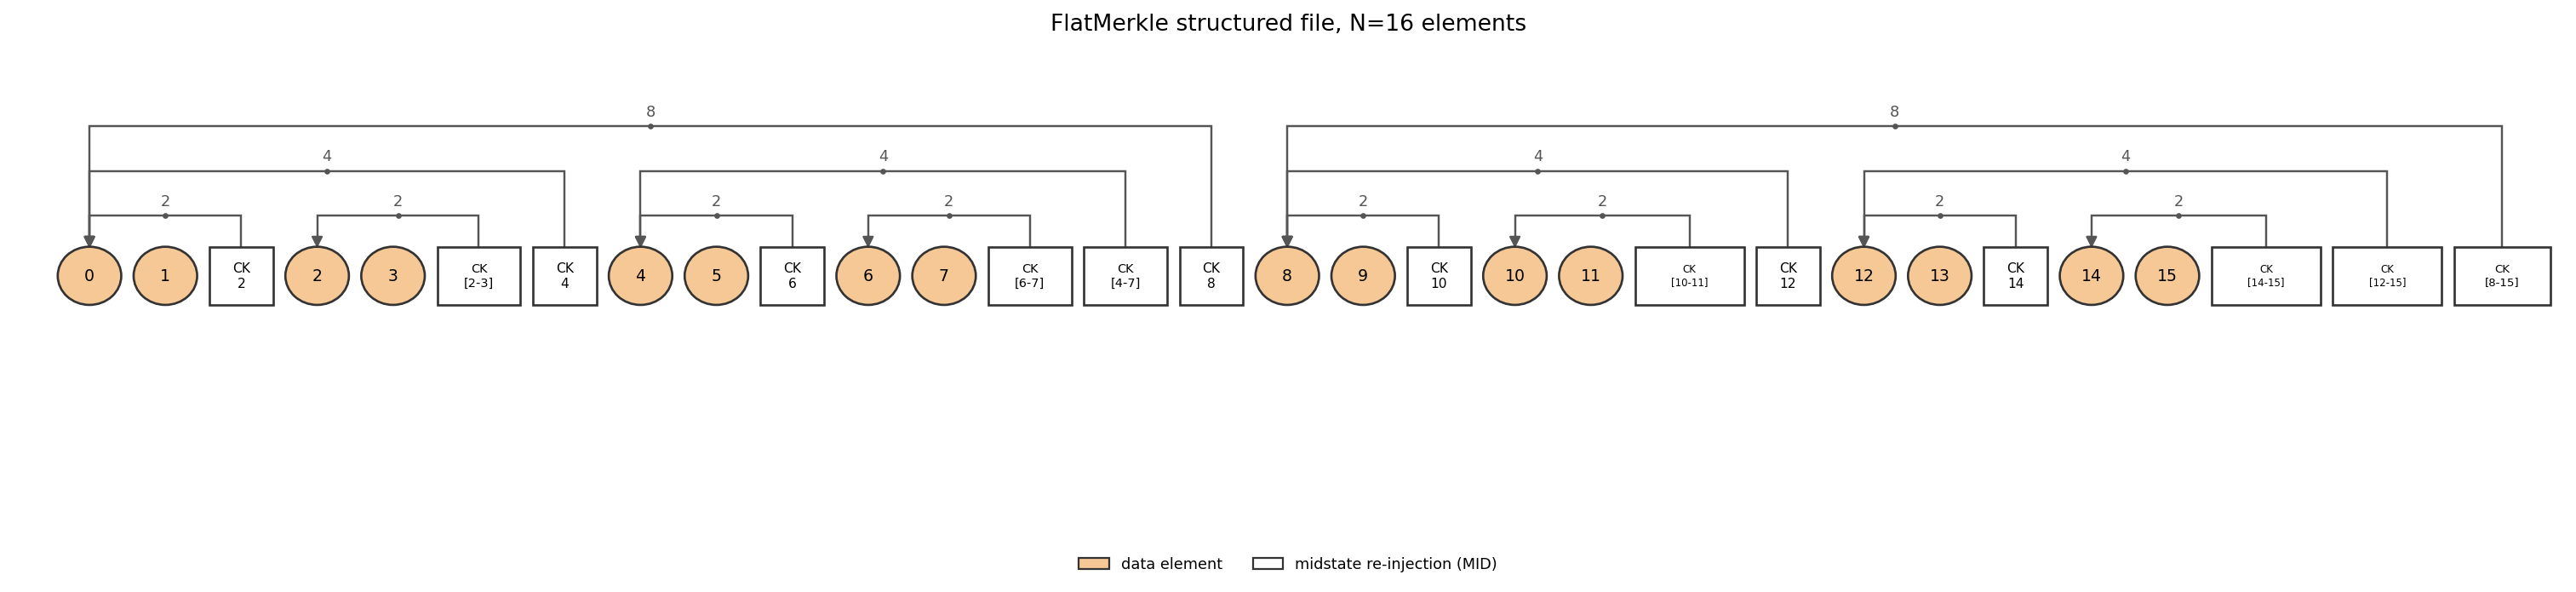
\includegraphics[width=\textwidth]{figures/structure_n16_plain.png}
\caption{The structured file for $N=16$ elements, in full: data elements as
circles, $\mathrm{MID}$ (checkpoint re-injection) blocks as boxes labelled
by the rule above, and the distance-$2^k$ jump arcs implicit in the
recursion, drawn above the row with an arrowhead into the element each arc's
checkpoint traces back to. Read each box's label as naming the state that
box's arc points \emph{at} (the state \emph{entering} the block it opens),
not the block immediately to its left: the box labelled $\CK_4$, for
instance, physically \emph{contains} $\CK[0]=\mathrm{IV}$ and its arc points
back at element 0 -- it is promoting that value forward to be the
checkpoint of the block starting four elements later, not describing
anything about its own immediate neighbors.}
\label{fig:structure-n16}
\end{figure}

\subsection{Position formula}

To build or verify a proof for original index $a$ without materializing the
whole file, we need to know exactly where in the structured file's byte
stream element $a$'s content sits.

\begin{lemma}[Position formula]
\label{lem:position}
For any original index $a \in [0, N)$ -- even or odd, not only positions
that start a block -- the 0-indexed position of $D[a]$ in the structured
file is
\begin{equation}
\mathrm{position}(a) = 2a - \popcount(a),
\end{equation}
where $\popcount(a)$ is the number of 1-bits in the binary representation
of $a$.
\end{lemma}

\begin{proof}[Proof sketch]
By induction on the recursive structure of Section~\ref{sec:recursive-structure}.
Every element contributes exactly one data slot; every completed pair
contributes one additional $\mathrm{MID}$ slot, and more generally every
completed block at level $k \ge 1$ contributes one $\mathrm{MID}$ slot for
each level it closes. The number of $\mathrm{MID}$ slots emitted strictly
before position $a$ is exactly the number of block-closing boundaries
crossed on the way to $a$, which -- by the standard correspondence between
binary counter increments and block closures in a doubling recursive
structure -- equals $a - \popcount(a)$. Adding the $a$ data slots already
emitted gives $\mathrm{position}(a) = a + (a - \popcount(a)) = 2a -
\popcount(a)$.
\end{proof}

The prover and verifier of Section~\ref{sec:algorithm} never call
$\mathrm{position}(\cdot)$: they branch only on whether the target lies
below a block's midpoint. The formula is for a party holding only the raw
byte stream, who needs to locate $D[a]$ directly -- for example, to extract
an element from a downloaded Bitcoin annex (Section~\ref{sec:bitcoin-annex})
before building a proof. It is verified in the accompanying code against
the recursive construction for every index at every
$N \in \{4,8,16,32,64\}$.

\section{Inclusion proof: construction and verification}
\label{sec:algorithm}

\subsection{Two kinds of revealed value}

Besides the target pair's two raw data elements, every proof step reveals
exactly one 32-byte (in general, $w$-bit) state value per level of
recursion. Before saying what each reveal means, we need two pieces of
notation: the two snapshots of the running hash-chain state taken while a
block is built, and the notion of a \emph{sibling}.

\begin{definition}[Prewrap and ending]
\label{def:prewrap-ending}
Building $\mathrm{block}(a,k)$ (Section~\ref{sec:construction}) is a
prefix of the single, ongoing compression-chain computation for the whole
file, and it ends with one specific compression call: the one that applies
the block's own closing checkpoint re-injection, $\mathrm{MID}(a)$. Write
\[
\mathrm{prewrap}(a,k) = \text{the running state \emph{immediately before}
that final call,}
\]
i.e.\ right after every element and every nested $\mathrm{MID}$ belonging to
$\mathrm{block}(a,k)$ \emph{other than its own closing one} has been hashed,
and write
\[
\mathrm{ending}(a,k) = \C\big(\mathrm{prewrap}(a,k),\ \mathrm{MID}(a)\big)
\]
for the state \emph{immediately after} that call. Both are snapshots of the
same single running state used to build the whole file -- they are not
separately computed side channels -- taken one compression call apart, on
either side of $\mathrm{block}(a,k)$'s own closing step. (A checkpoint
$\CK[a']$ for $a' \ne 0$, Section~\ref{sec:construction}, is always equal
to $\mathrm{ending}(a,k)$ for whichever block happens to finish immediately
before position $a'$ begins; the one exception is $\CK[0] = \mathrm{IV}$,
which is not any block's $\mathrm{ending}$.)
\end{definition}

\paragraph{The generic step.} Before a concrete example, here is the same
pattern once, abstractly, for a single call $\mathrm{block}(a,k)$ with
$k \ge 2$. Every line below is one of exactly two kinds, and the rule is
about the \emph{word}, not the font: a line that says \textbf{emit} writes
bytes to the file and feeds them into the hash chain; every other line
merely \emph{names} a value the running state already has, and writes
nothing. (\emph{Execute} is a third thing, strictly speaking -- a recursive
call that itself expands into a sequence of exactly this same shape, one
level down -- so it is set in plain text, neither bold nor colored.) To
make the two real kinds easy to tell apart at a glance even where the
line is mostly math, \emph{emit} lines are \textbf{bold black}, and every
value-naming line is \snap{shown in gray}:

\begin{enumerate}[itemsep=1pt, parsep=0pt, topsep=4pt]
\item \snap{if not already set: $\CK[a] := $ state}
\item execute $\mathrm{block}(a,\, k{-}1)$
\item execute $\mathrm{block}(a + 2^{k-1},\, k{-}1)$
\item \snap{$\mathrm{prewrap}(a,k) := $ state}
\item \textbf{emit $\mathrm{MID}(a)$}
\item \snap{$\mathrm{ending}(a,k) := $ state}
\end{enumerate}

The base case $k=1$ is the same six steps with two data emissions,
\textbf{emit $D[a]$} and \textbf{emit $D[a{+}1]$}, standing in for the two
recursive calls (steps 2--3). Every call to $\mathrm{block}(\cdot,\cdot)$
made anywhere in the whole construction -- there are exactly $N-2$ of them,
one per $\mathrm{MID}$ emission -- follows one of these two shapes.

The $N=8$ example below is exactly what you get from inlining every one of
the $N-2=6$ calls that construction makes, in the order they actually
execute, down to the individual data elements.

\paragraph{Example: the full build sequence for $N=8$.} To make
Definition~\ref{def:prewrap-ending} concrete, here is the complete,
real sequence of events building the structured file for a small $N=8$
example ($D[0..7]$), exactly as produced by the reference implementation,
using the same \textbf{bold} (emit) / \snap{gray} (value-naming only)
convention as above:

\begin{enumerate}[itemsep=1pt, parsep=0pt, topsep=4pt]
\item \snap{$\CK[0] := \mathrm{IV}$}
\item \textbf{emit $D[0]$}
\item \textbf{emit $D[1]$}
\item \snap{$\mathrm{prewrap}(0,1) :=$ state}
\item \textbf{emit $\mathrm{MID}(0)$} \hfill (bytes $= \mathrm{pad}_b(\CK[0])$)
\item \snap{$\mathrm{ending}(0,1) :=$ state}
\item \snap{$\CK[2] :=$ state} \hfill ($= \mathrm{ending}(0,1)$)
\item \textbf{emit $D[2]$}
\item \textbf{emit $D[3]$}
\item \snap{$\mathrm{prewrap}(2,1) :=$ state}
\item \textbf{emit $\mathrm{MID}(2)$} \hfill (bytes $= \mathrm{pad}_b(\CK[2])$)
\item \snap{$\mathrm{ending}(2,1) :=$ state}
\item \snap{$\mathrm{prewrap}(0,2) :=$ state} \hfill ($= \mathrm{ending}(2,1)$)
\item \textbf{emit $\mathrm{MID}(0)$ (again)} \hfill (bytes $=
  \mathrm{pad}_b(\CK[0])$, same bytes as step 5)
\item \snap{$\mathrm{ending}(0,2) :=$ state}
\item \snap{$\CK[4] :=$ state} \hfill ($= \mathrm{ending}(0,2)$)
\item \textbf{emit $D[4]$}
\item \textbf{emit $D[5]$}
\item \snap{$\mathrm{prewrap}(4,1) :=$ state}
\item \textbf{emit $\mathrm{MID}(4)$} \hfill (bytes $= \mathrm{pad}_b(\CK[4])$)
\item \snap{$\mathrm{ending}(4,1) :=$ state}
\item \snap{$\CK[6] :=$ state} \hfill ($= \mathrm{ending}(4,1)$)
\item \textbf{emit $D[6]$}
\item \textbf{emit $D[7]$}
\item \snap{$\mathrm{prewrap}(6,1) :=$ state}
\item \textbf{emit $\mathrm{MID}(6)$} \hfill (bytes $= \mathrm{pad}_b(\CK[6])$)
\item \snap{$\mathrm{ending}(6,1) :=$ state}
\item \snap{$\mathrm{prewrap}(4,2) :=$ state} \hfill ($= \mathrm{ending}(6,1)$)
\item \textbf{emit $\mathrm{MID}(4)$ (again)} \hfill (bytes $=
  \mathrm{pad}_b(\CK[4])$, same bytes as step 20)
\item \snap{$\mathrm{ending}(4,2) :=$ state} \hfill (this is the file's raw
  chain state, before finalization)
\end{enumerate}

Two things are worth noticing. First, every \snap{gray, non-\textbf{emit}}
line is free: it is a name for a value the running state already has at
that point, not a separate computation and not a separate byte written
anywhere -- Definition~\ref{def:prewrap-ending}'s
$\mathrm{prewrap}$/$\mathrm{ending}$ pair is nothing more than \emph{before}
and \emph{after} labels for step~5 (or step~11, or~20, or~26 -- whichever
$\mathrm{MID}$ call is currently closing). Second, $\mathrm{MID}(0)$ is
emitted twice (steps 5 and
14) and $\mathrm{MID}(4)$ is emitted twice (steps 20 and 29): same
checkpoint bytes both times, but compressed against a different running
state each time, since the same original position can start more than one
nested block (here $a=0$ starts both $\mathrm{block}(0,1)$ and
$\mathrm{block}(0,2)$). This is exactly the mechanism that lets one
checkpoint, computed once, be reused at every level whose block happens to
start at that position -- the same reuse Definition~\ref{def:prewrap-ending}
already alludes to for $\CK[a']$ in general. (14 emitted items total -- 8
data, 6 $\mathrm{MID}$ -- matching $2N-2$ for $N=8$, Section~\ref{sec:construction}.)

\begin{definition}[Sibling]
\label{def:sibling}
At recursion level $k$, block $\mathrm{block}(a,k)$ has two children,
$\mathrm{block}(a, k-1)$ and $\mathrm{block}(a+h, k-1)$ with $h = 2^{k-1}$
(Section~\ref{sec:construction}). The target index $t$ lies in exactly one
of the two; call that one the \emph{target child}. The \textbf{sibling} (at
this level) is the other child -- the one \emph{not} containing $t$.
\end{definition}

Since the sibling does not contain the target, the proof does not recurse
into it: it reveals a single state value that stands in for the sibling's
whole contents. Which value depends on whether the sibling was built
before or after the target child:

\begin{description}
\item[\emph{Left sibling: becomes the new checkpoint.}] The sibling
  $\mathrm{block}(a,k-1)$ is already closed when the target child begins.
  Its closing state $\mathrm{ending}(a,k-1) = \CK_{a+2^{k-1}}$ is revealed
  and used directly as the checkpoint that starts the evaluation of the
  target child.
\item[\emph{Right sibling: combined with the verified value.}] The sibling
  $\mathrm{block}(a+h,k-1)$ is built after the target child. The proof
  reveals its \emph{pre}-closing state $\mathrm{prewrap}(a+h,k-1)$, not its
  ending, and the verifier performs the sibling's closing fold itself,
  using $\mathit{left\_end}$, its own result for the target child, as the
  checkpoint. Revealing $\mathrm{ending}(a+h,k-1)$ instead would make the
  final check independent of $\mathit{left\_end}$, so any target data below
  this level would verify (Remark~\ref{rem:prewrap-bug}). For $k-1 \ge 2$,
  $\mathrm{prewrap}(a+h,k-1)$ is the ending of the sibling's own right child
  and carries the label $\CK_{[a+h+2^{k-2},\,a+h+2^{k-1}-1]}$
  (Section~\ref{sec:construction}); for $k-1=1$ it is unlabelled.
\end{description}

Concretely, the fold-in step in the second case computes
\begin{equation}
\C\big(\mathrm{prewrap}(a{+}h,k{-}1),\ \mathrm{pad}_b(\mathit{left\_end})\big),
\label{eq:foldin}
\end{equation}
and in a genuine proof $\mathit{left\_end} = \mathrm{ending}(a,k-1) =
\CK[a+h]$, the checkpoint that $\mathrm{block}(a+h,k-1)$'s closing
$\mathrm{MID}(a+h)$ re-injects, so by Definition~\ref{def:prewrap-ending}
\begin{equation}
\C\big(\mathrm{prewrap}(a{+}h,k{-}1),\ \mathrm{pad}_b(\CK[a+h])\big)
= \mathrm{ending}(a{+}h,k{-}1)
\end{equation}
exactly: the verifier recomputes the sibling's closing value from a
checkpoint it has itself just verified.

\paragraph{Closing $\mathrm{block}(a,k)$ itself.} After both children have
been accounted for, in left-to-right order, the state is
$v = \mathrm{prewrap}(a,k)$ in either case, and one further call closes
$\mathrm{block}(a,k)$ with its own checkpoint $\CK[a]$, passed down from
the level above:
\begin{equation}
\C\big(v,\ \mathrm{pad}_b(\CK[a])\big)
= \C\big(\mathrm{prewrap}(a,k),\ \mathrm{MID}(a)\big)
= \mathrm{ending}(a,k).
\label{eq:own-close}
\end{equation}
This is the last line of \textsc{EvalBlock} below,
\texttt{return C(right\_end, pad\_b(ckpt))}. Every level performs
Equation~\eqref{eq:own-close} once, in addition to resolving the sibling.
The two folds are easy to conflate in the pseudocode, but
Equation~\eqref{eq:foldin} closes the \emph{sibling} with $\CK[a{+}h]$,
while Equation~\eqref{eq:own-close} closes $\mathrm{block}(a,k)$ with
$\CK[a]$, one level up.

\subsection{Building a proof}

\begin{algorithm}[H]
\caption{$\textsc{BuildProof}(a_0, L)$ -- prover, given target pair start $a_0$}
\begin{lstlisting}[style=pseudo]
function Recurse(a, k, t):      # t = target index, in [a, a+2^k)
    if k = 1: return             # base case: no reveal here,
                                  # base pair always sent raw
    h := 2^(k-1)
    if t < a + h:                # target in left child
        Recurse(a, k-1, t)
        reveal prewrap(a+h, k-1)  # right sibling, not yet closed
    else:                         # target in right child
        reveal ending(a, k-1)     # left sibling, already closed
        Recurse(a+h, k-1, t)

h_top := 2^(L-1)
if a0 < h_top:
    Recurse(0, L-1, a0)
    reveal prewrap(h_top, L-1)
else:
    reveal ending(0, L-1)
    Recurse(h_top, L-1, a0)

return (D[a0], D[a0+1], reveals in the order emitted above)
\end{lstlisting}
\end{algorithm}

The proof carries $a_0$'s two data elements, not $a_0$ itself: the
verifier (Algorithm~3.3 below) always has its own trusted target
$\mathit{index}$ and derives the pair start from \emph{that}, never from
anything the proof claims -- $a_0$ is prover-side bookkeeping used to
build the reveal sequence, not part of the wire format.

\begin{lemma}[Index-independent proof size, for fixed $N$]
For every index $0 \le a < N = 2^L$, this procedure emits exactly $L-1$
reveals -- the same count for every index at that $N$, not merely an
average over indices. (Proof size is, as usual, still $O(\log N)$ in $N$
itself; the point here is that it does not additionally vary with
\emph{which} index is proven once $N$ is fixed.)
\end{lemma}

This follows directly from the algorithm: each of the $L-1$ recursive levels
above the base case emits exactly one reveal, regardless of which branch is
taken. (Section~\ref{sec:algorithm-cost} discusses \emph{verifier compute
cost}, which is \emph{not} constant across indices, even though proof size
is.)

\paragraph{Prover time and storage.} \textsc{BuildProof} as written treats
$\mathrm{ending}(a,k)$ and $\mathrm{prewrap}(a,k)$ as values simply
available to read off -- but, unlike the checkpoints $\CK[a]$, neither is a
literal byte range stored anywhere in the structured file
(Definition~\ref{def:prewrap-ending}): both are internal running-chain-
state snapshots that existed only transiently while the file was originally
built. Section~\ref{sec:construction}'s $O(\log N)$ working-memory claim is
for the \emph{build} step alone, and explicitly discards each checkpoint
once its block closes; it says nothing about the cost of later answering an
arbitrary proof request. Two honest options exist, with a real space/time
trade-off between them, and a deployment needs to pick one explicitly:
\begin{itemize}
\item \textbf{Cache every snapshot at build time.} Retain all $O(N)$
  intermediate $\mathrm{ending}$/$\mathrm{prewrap}$ values (one 32-byte, or
  in general $w$-bit, entry per $\mathrm{MID}$ emission) alongside the
  file, rather than discarding them. \textsc{BuildProof} then costs
  $O(\log N)$ time per request, matching proof \emph{size}, at the cost of
  $O(N)$ storage held indefinitely by whoever answers proof requests (in
  addition to the file itself). This is what the reference implementation
  does, for simplicity, exactly as Section~\ref{sec:construction} already
  notes for the analogous build-time choice.
\item \textbf{Recompute on demand.} Keep only the file bytes and answer
  each proof request by re-running the hash chain from the nearest
  available checkpoint up to the needed snapshot. Without any cached
  snapshots this costs up to $O(N)$ compression calls per proof request --
  no better than a full re-hash -- though a partial cache (e.g.\ one
  snapshot every $O(\sqrt{N})$ positions) trades a smaller, tunable storage
  budget against a correspondingly higher, but still sublinear, per-request
  recomputation cost.
\end{itemize}
Either way, the $O(\log N)$ figures emphasized elsewhere in this paper are
proof \emph{size} and verifier \emph{compute}, not prover storage: a
FlatMerkle prover that wants every request answered in $O(\log N)$ time,
matching the verifier's own cost, needs $O(N)$ storage to do it, the same
asymptotic footprint an equivalent Merkle-tree prover needs to keep the
whole tree (not just the root) on hand.

\subsection{Verifying a proof}

\begin{algorithm}[H]
\caption{$\textsc{EvalBlock}(a, k, t, \mathit{ckpt})$ -- verifier, symmetric to \textsc{Recurse}}
\label{alg:evalblock}
\begin{lstlisting}[style=pseudo]
function EvalBlock(a, k, t, ckpt):
    if k = 1:
        s := C(C(ckpt, D0), D1)      # the proof's base pair
        return C(s, pad_b(ckpt))     # re-inject checkpoint,
                                      # closing the base pair
    h := 2^(k-1)
    if t < a + h:                     # left branch
        left_end  := EvalBlock(a, k-1, t, ckpt)
        sib_prewrap := read next reveal
        right_end := C(sib_prewrap, pad_b(left_end))
                                       # fold in the value just verified
        return C(right_end, pad_b(ckpt))
    else:                              # right branch
        left_end  := read next reveal
        right_end := EvalBlock(a+h, k-1, t, left_end)
        return C(right_end, pad_b(ckpt))
\end{lstlisting}
\end{algorithm}

\begin{algorithm}[H]
\caption{$\textsc{Verify}(N, \Delta, \mathit{index}, \mathit{data}, \pi)$ -- top-level verifier}
\begin{lstlisting}[style=pseudo]
function Verify(N, Delta, index, data, pi):
    if N < 4 or N is not a power of two: return false   # domain: N = 2^L, L >= 2
    if index < 0 or index >= N: return false   # index out of range
    (D0, D1, reveals) := pi                    # reveals: a shared queue,
                                                # consumed front-to-back by
                                                # every "read next reveal"
                                                # line below and inside
                                                # EvalBlock (Section 3.3)
    a0 := index - (index mod 2)                # pair start, derived from
                                                # the verifier's OWN index --
                                                # NEVER taken from pi
    if index = a0: expected := D0 else: expected := D1
    if data != expected: return false           # supplied data disagrees with proof
    L := log2(N)
    h_top := 2^(L-1)
    if a0 < h_top:
        left_end := EvalBlock(0, L-1, a0, IV)     # consumes from reveals
        if reveals is empty: return false          # ran out before the top fold
        sib_prewrap := read next reveal
        raw_state := C(sib_prewrap, pad_b(left_end))
    else:
        if reveals is empty: return false
        left_end := read next reveal
        raw_state := EvalBlock(h_top, L-1, a0, left_end)
    if reveals is not empty: return false        # leftover reveals: malformed
    return finalize(raw_state, N) = Delta          # public length-padding + compare
\end{lstlisting}
\end{algorithm}

\begin{remark}[A natural-looking but insecure alternative: trusting a
proof-supplied pair start]
\label{rem:a0-bug}
A verifier might instead accept a pair start $a_0$ as part of the proof
itself, $\pi = (a_0, D_0, D_1, \mathit{reveals})$, and branch on whether
$\mathit{index} = a_0$ or $\mathit{index} = a_0+1$ to decide which of
$D_0, D_1$ is ``the'' claimed data -- exactly as \textsc{BuildProof}
computes $a_0$ internally. This is a genuine soundness hole, and a
collision-free one: \textsc{EvalBlock}'s recursion branches only on
whether the recursion target lies below a block's midpoint, and every
branch point above the base case compares against a power-of-two
threshold $h = 2^{k-1} \ge 2$, so the least-significant bit of the
recursion target never affects any branch decision -- indices $i-1$ and
$i$ (for odd $i$) take an \emph{identical} recursion path. An honest
proof for index $i-1$ carries $D_0 = D[i-1]$, and a verifier that trusts a
proof-supplied $a_0$ can be asked to check $(\mathit{index}=i,\
\mathit{data}=D[i-1], \pi)$ with $a_0$ relabelled to $i$ instead of $i-1$
(same $D_0, D_1$, same reveals, unchanged): the trusting verifier sees
$\mathit{index}=a_0$, sets $\mathit{expected} := D_0 = D[i-1]$, and
accepts -- reaching the genuine digest with no free-start collision at
all, since the recursion itself never used $a_0$ for anything but this one
comparison. The construction above avoids this by design: $a_0$ is never
read from $\pi$, only derived from the verifier's own $\mathit{index}$,
which the verifier is asking about in the first place and has no reason
to distrust. (The reference implementations already follow this
discipline -- \texttt{verify\_proof} derives its pair start solely from
the caller-supplied target index, and the wire-level \texttt{Proof} object
carries no separate pair-start field at all.)
\end{remark}

\textsc{EvalBlock}'s ``read next reveal'' lines share the same queue and
must reject if it is empty: too few reveals is as malformed as too many,
and an implementation that substitutes a default value for a missing
reveal reopens a gap of the same kind as Remark~\ref{rem:prewrap-bug}'s.
\textsc{Verify} first enforces the domain $N = 2^L$, $L \ge 2$
(Section~\ref{sec:construction}; for $N=2$ there is no top-level split),
then $\mathit{index} \in [0,N)$, derives $a_0$ from $\mathit{index}$
alone, checks $\mathit{data}$ against the element of the base pair that
$\mathit{index}$ selects, mirrors \textsc{BuildProof}'s top-level split
(there is no $\mathrm{MID}$ joining the two root blocks; the finalization
plays that role), rejects missing or leftover reveals, and only then
compares the finalized chain state with the digest. Both reference
implementations perform all of these checks; a re-implementation of
\textsc{EvalBlock}'s recursive core alone should add them.

\begin{remark}[A natural-looking but insecure alternative]
\label{rem:prewrap-bug}
A verifier might be tempted to compute the left branch's
$\mathit{left\_end}$ recursively (as required) but then discard it,
returning
\[
\C(\mathit{right\_end}, \mathrm{pad}_b(\mathit{ckpt}))
\]
without ever folding $\mathit{left\_end}$ into the check. This is a
genuine soundness hole: tampering with any value inside the left recursion
goes undetected, because the final check never actually depends on it.
The construction above avoids this by design (left branch of Algorithm~\ref{alg:evalblock}):
\[
\mathit{right\_end} := \C(\mathit{sib\_prewrap}, \mathrm{pad}_b(\mathit{left\_end})).
\]
The verifier must combine
the just-verified $\mathit{left\_end}$ with the revealed sibling
\emph{pre-close} state, not simply trust a separately revealed
\emph{post-close} state for the sibling and ignore what it just computed.
We recommend testing for exactly this class of omission directly --
flipping a single bit in every individually revealed value and confirming
rejection -- since it is the kind of gap that is easy to miss by
inspection alone.
\end{remark}

\subsection{Verifier compute cost varies by index; proof size does not}
\label{sec:algorithm-cost}

Although every proof has exactly $L-1$ reveals, the number of
compression-function calls the \emph{verifier} performs to check a proof is
not constant: it depends on how often the target's recursion path takes the
left branch (which costs 2 calls at that level: the fold, then the
checkpoint re-injection) versus the right branch (which costs 1 call: only
the checkpoint re-injection, since the sibling's closed value is used
as-is). For $N=32$ ($L=5$), measured directly against the real verifier
implementation:

\begin{table}[htbp]
\centering
\begin{tabular}{@{}lccccc@{}}
\toprule
Index & 0 & 8 & 15 & 23 & 30 \\
\midrule
Compression calls (incl.\ finalization) & 11 & 10 & 8 & 8 & 7 \\
\bottomrule
\end{tabular}
\caption{Verifier compression-function calls by target index, $N=32$. The
minimum, 7, is achieved by indices that take the cheap (right) branch at
every level; the maximum, 11, by index 0, which takes the left branch at
every level. In general the range is $[L+2,\ 2L+1]$ (including one constant
finalization call): the ratio $(2L+1)/(L+2)$ approaches, but never reaches,
$2\times$ as $L \to \infty$, and is strictly less than $2\times$ for every
finite $L$ (here, $L=5$: $11/7 \approx 1.57\times$) -- bounded, not
asymptotically growing relative to $L$.}
\label{tab:verifier-cost}
\end{table}

This asymmetry is a lever, not just a cost -- but the right way to describe
it is by \emph{bit pattern}, not by index magnitude. The exact cost is
$L + 2 + \#\{\text{zero bits among bits } 1..L{-}1 \text{ of the target}\}$,
which depends only on which of those bits are set, not on how large the
index is: for $N=32$, index 16 ($\texttt{10000}_2$) costs 10 -- almost as
expensive as index 0's 11, and no cheaper than index 8's 10 -- despite
being numerically closer to the ``high-index end'' than either. Index 30
($\texttt{11110}_2$) gets the minimum cost of 7 not because it is large,
but because its high-order bits happen to all be 1. The correct lever is
therefore: if the elements most likely to be queried are known in advance,
placing them at indices whose high-order bits are all 1 -- concretely, the
last few elements of the file -- favors the cheap, right-branch-heavy
verification path and reduces their average verification cost for free,
with no change to the construction or to the constant proof-size
guarantee. Since the whole range is bounded, $[L+2,\ 2L+1]$, the payoff of
this placement is at most a factor of roughly 2 and does not grow with
$N$ -- a genuine but modest optimization, not an asymptotic one.

\paragraph{A proof always discloses its whole base pair.}
\label{par:pair-disclosure}
\textsc{BuildProof} returns $D[a_0]$ and $D[a_0{+}1]$ unconditionally, where
$a_0 = a - (a \bmod 2)$ -- so a proof requested for target index $a$ always
discloses \emph{both} raw elements of its pair, not just $D[a]$: proving
index 7 necessarily also reveals element 6, whether or not anyone asked
about element 6. This is a real, semantic difference from an ordinary
Merkle proof, whose leaf hash need not expose any neighboring leaf, and it
is worth stating plainly rather than leaving implicit. It also affects the
size comparison in Section~\ref{sec:examples}'s table and
Section~\ref{sec:optimal-size}: with element size equal to the state width,
$D=W$, FlatMerkle's proof size $2D + (L-1)W$ and a same-shape Merkle
proof's size $LW + D$ come out numerically \emph{equal} -- but FlatMerkle's
byte count buys one fewer sibling hash \emph{and} one extra disclosed
element, not a strictly smaller disclosure. Anyone relying on FlatMerkle
proofs where the neighboring element's privacy matters should account for
this explicitly.

\section{Worked examples: $N=16$}
\label{sec:examples}

All examples in this section are built from 16 real 32-byte pseudorandom
elements, hashed with a toy but real compression function ($C(s,b) =
\mathrm{SHA256}(0x01 \,\Vert\, s \,\Vert\, b)$, 32-byte state and block --
so $b=w$, using the identity checkpoint encoding $\mathrm{pad}_w(x)=x$ of
Definition~\ref{def:padb} rather than the $b>w$ terminator-byte scheme),
and every proof below was independently re-verified, including confirming
that flipping a single bit anywhere in the target data, or in any one
revealed value, is rejected.

\begin{table}[htbp]
\centering
\begin{tabular}{@{}cccc@{}}
\toprule
Target index & Base pair proved (both) & Reveals & Proof size \\
\midrule
0  & $D[0],D[1]$   & 3 & 160 B \\
4  & $D[4],D[5]$   & 3 & 160 B \\
7  & $D[6],D[7]$   & 3 & 160 B \\
8  & $D[8],D[9]$   & 3 & 160 B \\
11 & $D[10],D[11]$ & 3 & 160 B \\
14 & $D[14],D[15]$ & 3 & 160 B \\
\bottomrule
\end{tabular}
\caption{Six representative target indices out of the 16 possible, spread
across the file; all 16 were checked and every one produces the same
\emph{constant} 160-byte proof ($2 \times 32$ bytes of raw pair data plus
$3 \times 32$ bytes of state reveals, $L-1=3$), since proof size does not
depend on which index is targeted (Section~\ref{sec:algorithm}). A proof
for target index $a$ always discloses \emph{both} raw elements of its base
pair, $D[a_0]$ and $D[a_0{+}1]$ -- proving index 7 necessarily also
discloses element 6 -- so the ``Base pair proved'' column names both
elements the proof exposes, not just the requested index (Section~\ref{sec:algorithm-cost}
discusses this). For comparison, a same-shape Merkle proof over 16 leaves
needs $\lceil \log_2 16 \rceil = 4$ sibling hashes (128 bytes) plus the
leaf's own preimage, and does \emph{not} disclose a neighboring leaf.}
\label{tab:examples-n16}
\end{table}

\subsection{Index 7 in detail}

Figure~\ref{fig:proof-n16-idx7} shows the full 16-element structured file
with the proof path for index 7 highlighted: the base pair $D[6],D[7]$,
and the checkpoint values $\CK_4$, $\CK_6$, and $\CK_{[12,15]}$, in the
order the proof actually reveals them.

\begin{figure}[htbp]
\centering
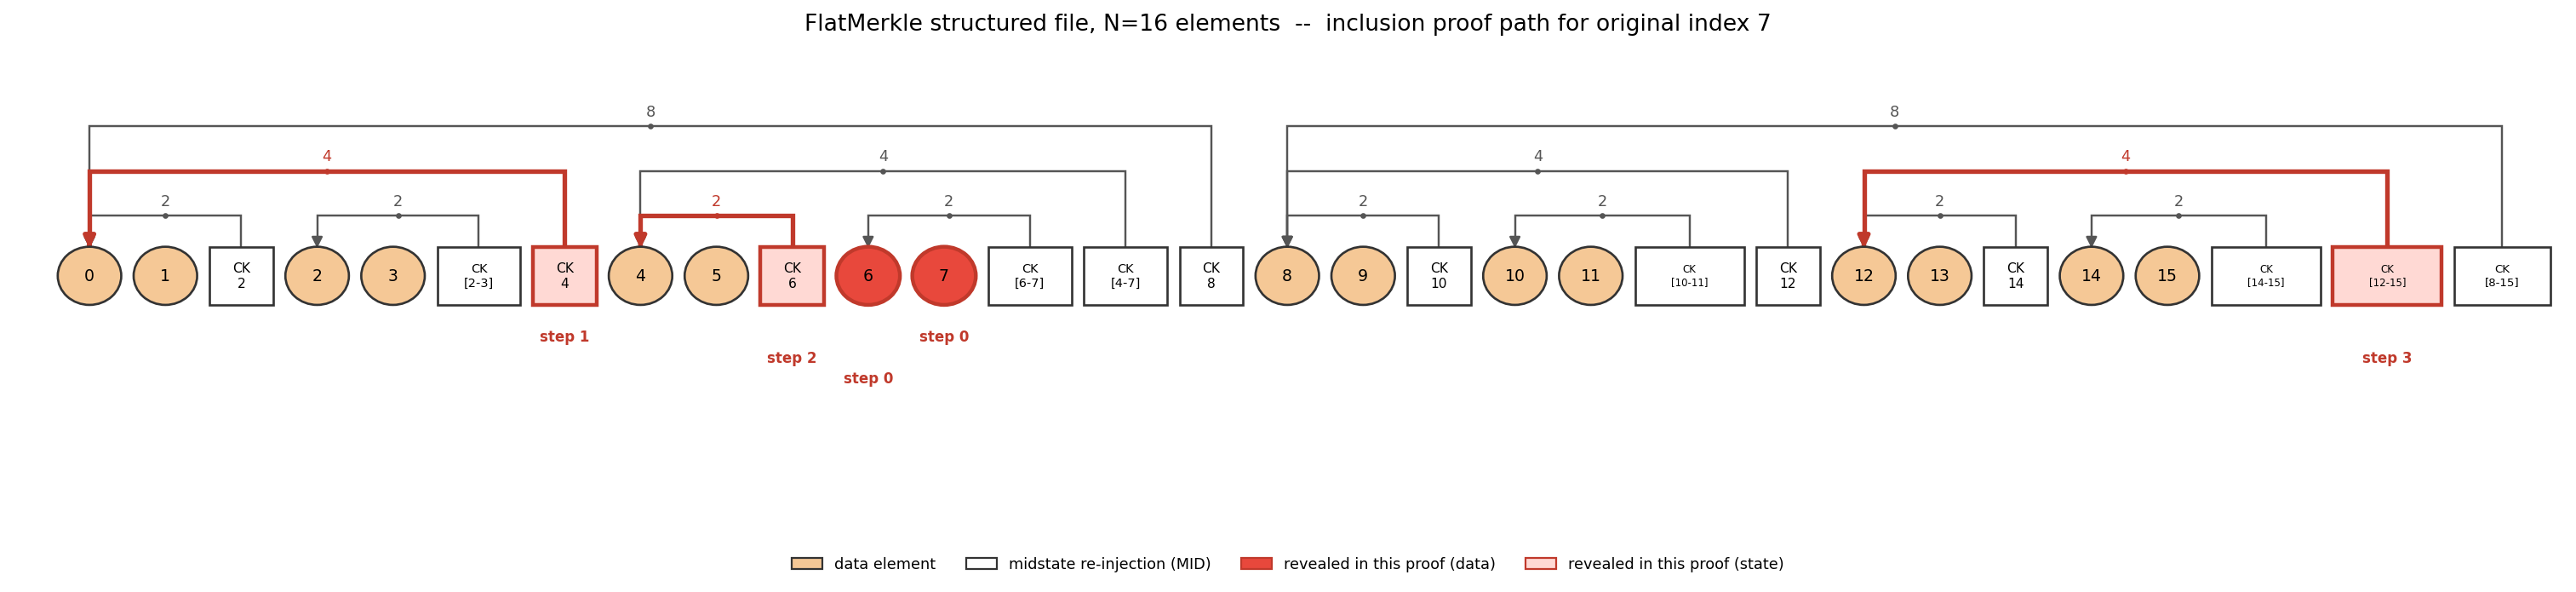
\includegraphics[width=\textwidth]{figures/proof_n16_idx7.png}
\caption{Structured file for $N=16$, proof path for index 7 highlighted in
red, numbered by the order each value is used.}
\label{fig:proof-n16-idx7}
\end{figure}

A natural question when first looking at Figure~\ref{fig:proof-n16-idx7} is
how the verifier gets from ``just after element 7'' to the digest: no arc
in the drawing runs directly from that point to the end. The reason is that
the verifier does not walk the file's own drawn jump-back arcs at all -- it
performs a straight, ordered fold of $\C(\cdot,\cdot)$ calls, each combining
the previous result with either the next raw element or the next revealed
checkpoint. Figure~\ref{fig:chain-n16-idx7} makes this explicit.

\begin{figure}[htbp]
\centering
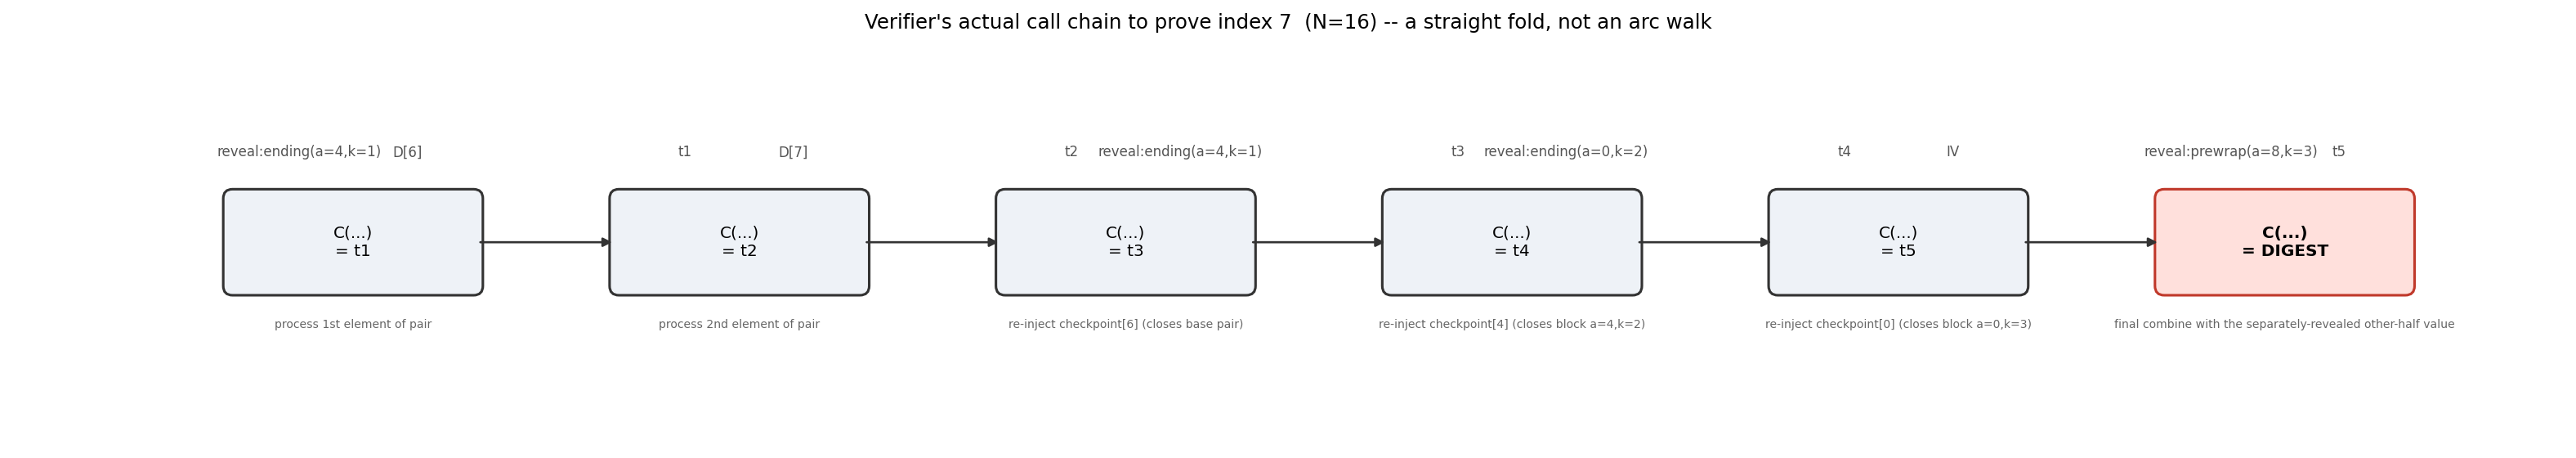
\includegraphics[width=\textwidth]{figures/chain_n16_idx7.png}
\caption{The verifier's actual sequence of compression-function calls for
index 7 -- a straight-line fold ending at the digest, not a walk along the
structured file's own arcs.}
\label{fig:chain-n16-idx7}
\end{figure}

Finally, Figure~\ref{fig:proof-stored-n16-idx7} shows the proof exactly as
it is stored and transmitted: a flat, ordered sequence of items with no tree
and no arcs, matching the compact wire format
\[
(D[a_0],\ D[a_0{+}1],\ \mathrm{reveals}[0..L{-}2]),
\]
where $a_0 = a - (a \bmod 2)$ is derived by the verifier from whichever
index it is asking about, never transmitted as part of the proof itself
(Remark~\ref{rem:a0-bug} explains why the proof must not carry its own
copy of $a_0$).

\begin{figure}[htbp]
\centering
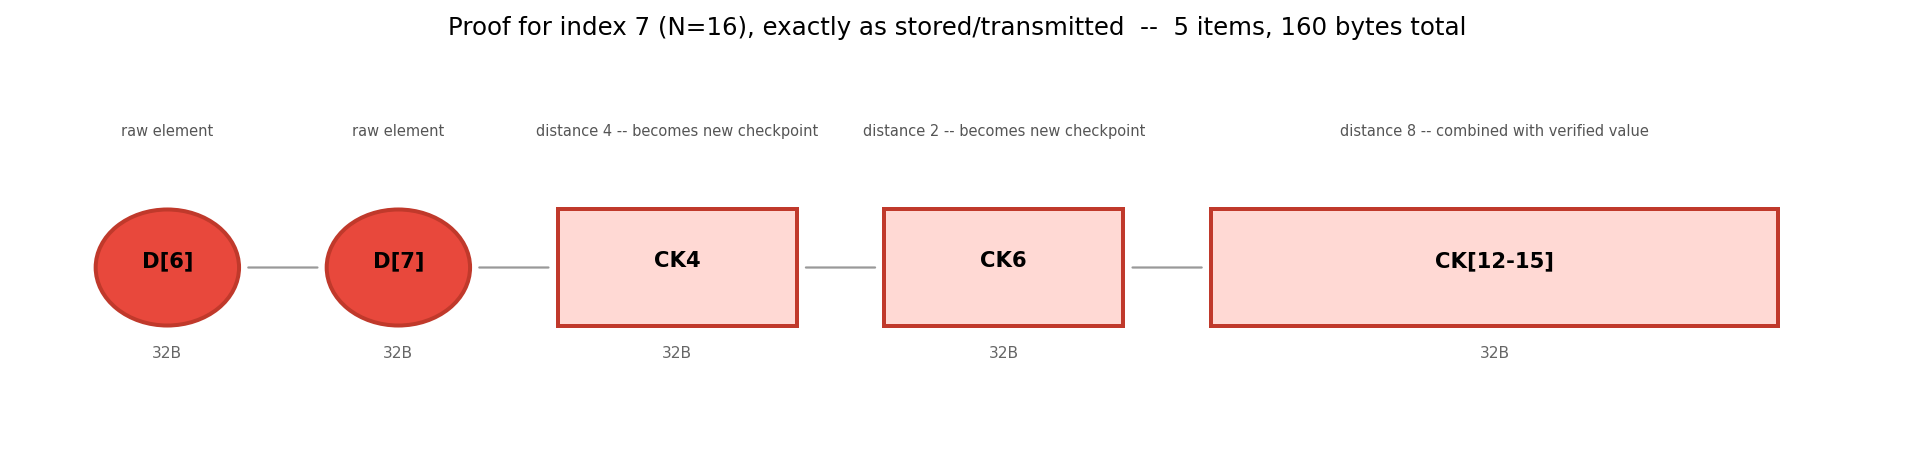
\includegraphics[width=0.8\textwidth]{figures/proof_stored_n16_idx7.png}
\caption{The index-7 proof exactly as stored: $D[6], D[7], \CK_4, \CK_6, \CK_{[12,15]}$ -- 5 items, 160 bytes, verified byte-for-byte against the real prover output.}
\label{fig:proof-stored-n16-idx7}
\end{figure}

\subsection{Reading the checkpoint labels}

$\CK_4$ and $\CK_6$ are each a single, unambiguous position: each is the
closing value ($\mathrm{ending}$) of a \emph{left}-child block, immediately
promoted to the checkpoint that starts the next block
(Section~\ref{sec:construction}). Using a single trailing index for this
kind of value (e.g.\ naming it by the last element it covers) would be
ambiguous, since different-sized blocks can share the same last-covered
index; the span notation avoids that collision by construction.

$\CK_{[12,15]}$ is different in kind, and worth reading carefully. The
third reveal is $\mathrm{prewrap}(8,3)$ -- the state right before
$\mathrm{block}(8,3)$'s own closing $\mathrm{MID}(8)$ folds in, \emph{not}
$\mathrm{ending}(8,3)$ (which is the file's own final raw chain state, and
is never revealed to any verifier, since it only exists after the
verifier's own last fold). $\mathrm{prewrap}(8,3)$ happens to equal
$\mathrm{ending}(12,2)$ -- $\mathrm{block}(8,3)$'s own right child's ending,
one level down -- since that child closes immediately before
$\mathrm{block}(8,3)$'s own $\mathrm{MID}(8)$ is written, so it names the
right child's span, $\CK_{[12,15]}$, \emph{not} $\mathrm{block}(8,3)$'s own
span $\CK_{[8,15]}$ (which would name a value -- $\mathrm{ending}(8,3)$ --
this proof never touches at all). The verifier does not receive
$\CK_{[12,15]}$ as a promoted checkpoint the way it does $\CK_4$ or
$\CK_6$: it folds this reveal together with $D[6],D[7]$'s already-verified
result to \emph{compute} $\mathrm{block}(8,3)$'s own closing value, which
the verifier itself performs as the last fold in
Figure~\ref{fig:chain-n16-idx7}.

\section{Security}
\label{sec:security}

\subsection{Assumptions}

\begin{assumption}[Free-start collision resistance]
\label{ass:freestart}
It is computationally infeasible to find $(s_1, b_1) \ne (s_2, b_2) \in
\{0,1\}^w \times \{0,1\}^b$ with $\C(s_1,b_1) = \C(s_2,b_2)$.
\end{assumption}

This differs from the collision resistance ordinarily assumed of a hash
function $H$, which fixes the starting state to $\mathrm{IV}$ and only
requires hardness of finding two distinct \emph{messages} colliding under
that fixed start. Assumption~\ref{ass:freestart} is strictly stronger: it
must hold for \emph{adversarially chosen} starting states, because a
FlatMerkle verifier accepts several state values as untrusted input (the
proof's reveals) and only ever ties them to the truth via later equality
checks against the published digest -- never by re-deriving them from
$\mathrm{IV}$ itself. This is exactly the property the construction needs,
and we state it as a distinct, named assumption rather than assume it
follows automatically from ordinary collision resistance of $H$; in
general it does not -- free-start collision resistance of a
Davies--Meyer-style compression step is a materially stronger, separately
studied property~\citep{dobbertin1996}.

\begin{remark}[This assumption has failed for real, deployed compression
functions]
\label{rem:freestart-history}
The gap between Assumption~\ref{ass:freestart} and ordinary collision
resistance is not merely theoretical. Free-start collisions were found for
MD5's compression function in 1996~\citep{dobbertin1996}, years before any
collision was known for MD5 itself, and for the full SHA-1 compression
function in 2015~\citep{stevens2015shappening} -- two years before the
first ordinary SHA-1 collision (SHAttered, 2017). A FlatMerkle instance
built on SHA-1 was therefore already insecure in 2015, at a time when
SHA-1 was still considered safe for ordinary hashing by most practitioners.
Assumption~\ref{ass:freestart} should be checked against the
free-start-collision literature for the specific compression function in
use, not against that function's ordinary collision-resistance track
record. For SHA-256, this paper's main instantiation, the best published
result we are aware of is a practical \emph{semi}-free-start collision
for $39$ of its $64$ steps \citep{li2024sha2}; no free-start collision is
known for the full compression function. For BLAKE2b, used in
Section~\ref{sec:rollup-eth}, Guo et al.\ report weaknesses of the
compression function when its \emph{entire} 16-word internal state is
chosen \citep{guo2013blake2}; a FlatMerkle verifier only lets an adversary
choose the 8-word chaining value and the message block, and fixes the
remaining inputs itself (see Section~\ref{sec:rollup-eth}), but this
margin is narrower than for SHA-256 and should be reassessed before
deployment.
\end{remark}

\begin{assumption}[Raw compression-function access]
\label{ass:mdaccess}
The hash function $H$ is built from $\C$ via the standard Merkle--Damg\aa rd
iteration with a public finalization, and both prover and verifier have
direct access to $\C$ itself (not merely to $H$).
\end{assumption}

This rules out hash functions where the internal chaining step is not
separately exposed or well-defined (e.g.\ most sponge constructions --
see the discussion of adapting FlatMerkle to Keccak-256 in
Section~\ref{sec:conclusion}), and is satisfied by the Merkle--Damg\aa rd
family generally, including SHA-256, SHA-1, and MD5. Satisfying
Assumption~\ref{ass:mdaccess} says nothing about whether
Assumption~\ref{ass:freestart} also holds for a given member of that
family -- see Remark~\ref{rem:freestart-history}.

\begin{remark}[No domain separation between data and $\mathrm{MID}$ blocks]
\label{rem:domain-sep-bit}
A data element may be byte-identical to some $\mathrm{MID}$ block; nothing
in the construction prevents it. This does not affect
Theorems~\ref{thm:soundness} or~\ref{thm:binding}: which positions are
data and which are checkpoints is fixed by $(\mathit{index}, N)$ before any
byte is examined, never inferred from content. A deployment wanting an
extra margin can still tag $\mathrm{MID}$ blocks, provided the tag uses
the $b-w$ bits that $\mathrm{pad}_b$ leaves free (256 bits for SHA-256)
and application data is escaped to avoid the same pattern. Overwriting any
of the checkpoint's own $w$ bits instead would break the injectivity of
$\mathrm{pad}_b$, which both theorems use. In a Bitcoin annex, any such
convention must be known to anyone parsing the raw annex bytes, since
consensus does not distinguish the two.
\end{remark}

\subsection{Soundness}

All three security arguments in this section -- soundness, binding, and
fraud-proof soundness (Section~\ref{sec:fraud-proofs}) -- compare two
executions of the same verifier recursion that reach the same output, and
propagate that equality from outputs back to inputs. The one subtlety is
the checkpoint argument: in a right branch, \textsc{EvalBlock} seeds the
child with a \emph{revealed} value, not with its own $\mathit{ckpt}$, so a
naive ``descend and compare'' walk cannot assume a child's checkpoint
argument is already known to agree in both executions. We therefore state
the induction once, with a hypothesis that quantifies over
\emph{unequal} checkpoint arguments, in a form general enough to cover the
modified evaluator the fraud-proof verifier uses.

Fix $N = 2^L$, a target $t$, and a set $V$ of $t$'s own containing levels
(Definition~\ref{def:anchored} below; $V = \emptyset$ for ordinary
verification). $\textsc{EvalBlock}_V$ is \textsc{EvalBlock} except that, at
each level $(a,k) \in V$, its own closing fold uses a supplied $b$-bit
string $m_{(a,k)}$ in place of $\mathrm{pad}_b(\mathit{ckpt})$;
$\textsc{EvalBlock}_\emptyset = \textsc{EvalBlock}$.

\begin{definition}[Anchored level]
\label{def:anchored}
For $1 \le k \le L-1$ let $a_k = \lfloor t/2^k \rfloor 2^k$, so that
$\mathrm{block}(a_k,k)$ is $t$'s containing block at level $k$. The
checkpoint argument at level $k$ is \emph{anchored} (with respect to $t$
and $V$), written $\mathrm{bnd}(k)$, if
\[
\mathrm{bnd}(1) = \text{true}, \qquad
\mathrm{bnd}(k) = \big[(a_k,k) \notin V\big] \ \vee\
\big[\mathrm{bit}_{k-1}(t) = 0 \ \wedge\ \mathrm{bnd}(k-1)\big]
\quad (2 \le k \le L-1),
\]
and, additionally, $\mathrm{bnd}(L-1) = \text{true}$ whenever $t < 2^{L-1}$.
In words: a checkpoint is anchored if it survives in its own closing fold;
or if the level takes the left branch, in which case the same value is
passed down to the child and the question recurses; the base case is
always anchored because $\C(\mathit{ckpt}, d_0)$ consumes it whether or not
its closing fold is substituted; and the top-level left root's checkpoint
is the public constant $\mathrm{IV}$, fixed by the verifier itself. With
$V = \emptyset$ every level is anchored.
\end{definition}

\begin{lemma}[Extraction]
\label{lem:extraction}
Let $1 \le k \le L-1$ and consider two executions of
$\textsc{EvalBlock}_V(a_k, k, t, \cdot)$ with checkpoint arguments
$\mathit{ckpt}_1, \mathit{ckpt}_2$ -- not assumed equal -- and their own
reveals, base elements and substituted strings. If both return the same
value, then either a free-start collision in $\C$ can be extracted from the
two executions with $O(k)$ compression calls, or all of the following
hold: (i) both consumed the same base elements $d_0, d_1$, the same
left-branch sibling reveals, and the same substituted strings
$m_{(a_j,j)}$ for every $(a_j,j) \in V$, $j \le k$; (ii) for every $j \le
k$ with $\mathrm{bnd}(j)$, the two executions' checkpoint arguments at
level $j$ coincide -- in particular $\mathit{ckpt}_1 = \mathit{ckpt}_2$ if
$\mathrm{bnd}(k)$, and every right-branch reveal that seeds an anchored
child coincides.
\end{lemma}

\begin{proof}
Induction on $k$. Every invocation ends with one compression call
$\C(x_i, c_i)$, where $c_i = \mathrm{pad}_b(\mathit{ckpt}_i)$ if
$(a_k,k) \notin V$ and $c_i = m_{(a_k,k),i}$ otherwise. Equal outputs give
either a collision or $x_1 = x_2$ and $c_1 = c_2$; in the first sub-case
injectivity of $\mathrm{pad}_b$ (Definition~\ref{def:padb}) gives
$\mathit{ckpt}_1 = \mathit{ckpt}_2$, in the second the substituted strings
agree.

\emph{Base, $k=1$:} $x_i = \C(\C(\mathit{ckpt}_i, d_{0,i}), d_{1,i})$, so
equal $x$ gives a collision or $d_{1,1} = d_{1,2}$ and equal inner outputs,
which in turn gives a collision or $\mathit{ckpt}_1 = \mathit{ckpt}_2$ and
$d_{0,1} = d_{0,2}$ -- regardless of $V$, matching $\mathrm{bnd}(1)$.

\emph{Left branch} ($\mathrm{bit}_{k-1}(t) = 0$): $x_i =
\C(s_i, \mathrm{pad}_b(\ell_i))$ with $s_i$ the sibling's revealed prewrap
and $\ell_i = \textsc{EvalBlock}_V(a_k, k{-}1, t, \mathit{ckpt}_i)$. Equal
$x$ gives a collision or $s_1 = s_2$ and $\ell_1 = \ell_2$; the induction
hypothesis applied to the child (whose checkpoint argument is the
\emph{same} $\mathit{ckpt}_i$) gives a collision or (i)--(ii) below level
$k$, including $\mathit{ckpt}_1 = \mathit{ckpt}_2$ if $\mathrm{bnd}(k-1)$.
Together with the closing fold: $\mathit{ckpt}$ is pinned iff $(a_k,k)
\notin V$ or $\mathrm{bnd}(k-1)$, which is $\mathrm{bnd}(k)$.

\emph{Right branch} ($\mathrm{bit}_{k-1}(t) = 1$): $x_i =
\textsc{EvalBlock}_V(a_k + 2^{k-1}, k{-}1, t, r_i)$, where $r_i$ is a
\emph{revealed} value, not $\mathit{ckpt}_i$. The induction hypothesis
gives a collision or (i)--(ii) below level $k$, including $r_1 = r_2$ if
$\mathrm{bnd}(k-1)$. Here $\mathit{ckpt}_i$ appears \emph{only} in the
closing fold, so it is pinned iff $(a_k,k) \notin V$, which is again
$\mathrm{bnd}(k)$.

Each level inspects $O(1)$ calls, so the collision, if any, is found within
$O(k)$ calls by recomputing both executions.
\end{proof}

The only place the top-level split of \textsc{Verify} differs from a
generic level is that the left root is seeded with $\mathrm{IV}$ in both
executions -- which is why Definition~\ref{def:anchored} marks it anchored
unconditionally -- and that the top-level sibling's closing fold,
$\C(\mathit{sib\_prewrap}, \mathrm{pad}_b(\mathit{left\_end}))$, is never
substituted. Finalization is one further fixed public suffix of compression
calls on blocks determined only by $N$ (for SHA-256 and $64$-byte items,
exactly one padding block), so equal digests give either a collision or
equal raw chain states. Combining these with Lemma~\ref{lem:extraction}
gives the following top-level statement, used by every theorem below.

\begin{corollary}[Top-level extraction]
\label{cor:top-extraction}
If two executions of \textsc{Verify} (with $V = \emptyset$), or of the
fraud-proof fold of Section~\ref{sec:fraud-proofs} (with the same $t$ and
$V$), both for the same $N$ and target $t$, finalize to the same digest,
then either a free-start collision in $\C$ can be extracted with $O(\log
N)$ compression calls, or the two executions consumed the same $d_0, d_1$,
the same left-branch reveals, the same substituted strings, and agree on
the checkpoint argument at every anchored level of $t$'s path. With $V =
\emptyset$ this means the two proofs are identical.
\end{corollary}

\begin{theorem}[Soundness]
\label{thm:soundness}
Under Assumptions~\ref{ass:freestart} and~\ref{ass:mdaccess}, no adversary
can produce $(\mathit{index}, \mathit{data}, \pi)$ accepted by
\textsc{Verify} against a genuine digest $\Delta$, where $\mathit{data}$
disagrees with the true element $D[\mathit{index}]$ that $\Delta$ actually
commits to, without also producing a free-start collision in $\C$.
\end{theorem}

\begin{proof}
Let $\pi^*$ be the genuine proof for $\mathit{index}$, built by
\textsc{BuildProof} against the real file; it is accepted
(Section~\ref{sec:completeness}). Suppose an adversary's
$(\mathit{index}, \mathit{data}, \pi)$ is also accepted, with
$\mathit{data} \ne D[\mathit{index}]$. Both executions use the same
$\mathit{index}$ and $N$, hence the same target pair start $a_0$ and the
same branch decisions, and both finalize to $\Delta$.
Corollary~\ref{cor:top-extraction} with $V = \emptyset$ yields either a
free-start collision or $\pi = \pi^*$; in the latter case \textsc{Verify}
selects $\mathit{data}$ from the same $(d_0,d_1)$ by the same parity of
$\mathit{index}$, so $\mathit{data} = D[\mathit{index}]$, a contradiction.
\end{proof}

\subsection{Completeness}
\label{sec:completeness}

Completeness is immediate from construction: for any index and any honestly
built file, \textsc{EvalBlock} run against the reveals produced by
\textsc{BuildProof} recomputes, level by level, exactly the same sequence of
compression calls the builder performed -- by inspection of the two
algorithms in Section~\ref{sec:algorithm}, they are symmetric by design.
This was also confirmed empirically: every index of every tested $N \in
\{4,8,16,32,64\}$ verifies successfully against a genuinely built file.

\subsection{Binding: what an accepting proof actually certifies}
\label{sec:binding}

It might seem that Theorem~\ref{thm:soundness}'s technique establishes
something stronger than it actually does: that for \emph{any} byte string
$F'$ a publisher chooses to publish -- canonically built or not -- no
accepting proof could name data other than the bytes genuinely present at
$\mathrm{position}(\mathit{index})$ in $F'$. That claim is false, and
Remark~\ref{rem:layout-forgery} below gives a working forgery against it.
What Theorem~\ref{thm:soundness}'s technique actually establishes, for an
arbitrary (possibly non-canonical) $F'$, is a strictly weaker and correct
property: \emph{binding}, not \emph{provenance}.

\begin{theorem}[Binding]
\label{thm:binding}
Fix $N = 2^L$ ($L \ge 2$, the domain \textsc{Verify} itself checks -- see
Section~\ref{sec:algorithm}), any published digest $\Delta'$, and any
$\mathit{index} \in [0, N)$. Under Assumption~\ref{ass:freestart}, there is
at most one value $\mathit{data}$ for which some proof $\pi$ makes
\textsc{Verify} accept $(N, \mathit{index}, \mathit{data}, \pi)$ against
$\Delta'$ -- regardless of whether $\Delta'$ commits to a canonically built
file. ($N$ is fixed throughout, not just $\Delta'$ and $\mathit{index}$,
because \textsc{Verify}'s recursion structure -- how many levels deep it
goes, and where each branch falls -- is itself a function of $N$; two
different $N$ values would in general give two entirely different
recursions over the same $\Delta'$, so the claim is only meaningful, and
only proved, for one $N$ at a time.)
\end{theorem}

\begin{proof}
Suppose two accepting triples $(\mathit{index}, \mathit{data}_1, \pi_1)$
and $(\mathit{index}, \mathit{data}_2, \pi_2)$, both against the same fixed
$N$, verify against $\Delta'$, with $\mathit{data}_1 \ne \mathit{data}_2$.
Corollary~\ref{cor:top-extraction} (with $V = \emptyset$) only ever
compares two \emph{accepting executions} against each other; it never
assumes either was built by the honest \textsc{Build} procedure, only that
both recursion structures are fixed by $(\mathit{index}, N)$ -- identical
here, since $N$ is fixed -- and that both reach the same $\Delta'$. It
therefore yields either a free-start collision or $\pi_1 = \pi_2$, hence
$\mathit{data}_1 = \mathit{data}_2$, contradicting the assumption.
\end{proof}

\begin{remark}[Binding does not imply the accepted value matches $F'$'s own bytes -- a working forgery]
\label{rem:layout-forgery}
Take a target $\mathit{index}$ in the left half of the file. The verifier's
very last step is $\mathit{raw\_state} = \C(r,\ \mathrm{pad}_b(y))$, where
$y$ is the value the left-half recursion just computed and $r$ is an
\emph{unverified} reveal -- nothing above binds $r$ to anything. In a
canonically built file, the file's own last 64 bytes are exactly
$\mathrm{MID}(2^{L-1}) = \mathrm{pad}_b(\CK[2^{L-1}]) = \mathrm{pad}_b(\mathrm{ending}(0,L-1))$,
i.e.\ the true ending of the real left-half data -- but nothing forces a
\emph{publisher} to write that value there. A publisher can instead:
pick arbitrary fake $D[0], D[1]$ and arbitrary fake inner reveals; run the
left-half recursion forward on this fake path to obtain some $y_{\mathit{fake}}$;
write $\mathrm{pad}_b(y_{\mathit{fake}})$, instead of the true checkpoint, as
the file's actual last 64 bytes; and separately place whatever real data
they like at $\mathrm{position}(0)$ elsewhere in the file. Reading off the
true chain state $r$ entering that last block -- a public quantity, computable
by anyone holding $F'$, no secret or collision required -- the fake
$(D[0], D[1], \text{reveals})$ now verifies against the real, published
$\Delta' = H(F')$, even though the bytes genuinely sitting at
$\mathrm{position}(0)$ in $F'$ are something else entirely. This costs
\emph{no} free-start collision: it is exactly the deviation
Theorem~\ref{thm:binding} does not rule out (both fake and genuine
$\mathit{index}=0$ claims cannot \emph{simultaneously} be accepting, by
binding -- but binding says nothing about which one, if either, matches
what a reader who simply parses $F'$ would call ``the data at
$\mathrm{position}(0)$''). Confirmed against the real SHA-256 reference
implementation (\texttt{loglink\_annex.py}): a file identical to a
canonical one except for a single 32-byte checkpoint, whose SHA-256 is a
completely ordinary digest, admits an accepting proof for forged
$\mathit{index}=0$ data.
\end{remark}

An accepting proof therefore certifies membership in \emph{the dataset
defined by the file's own accepting proofs}, not ``the bytes at
$\mathrm{position}(i)$ of $F'$'' as literally parsed off the byte string --
the two coincide only when $F'$ is canonically built to begin with, a
property Theorem~\ref{thm:binding} says nothing about and which cannot be
checked from $\Delta'$ alone in less than $O(N)$ work. Section~\ref{sec:fraud-proofs}
gives that missing check.

\subsection{Fraud proofs: proving a published file is not canonically built}
\label{sec:fraud-proofs}

Binding rules out equivocation but, as Remark~\ref{rem:layout-forgery}
shows, does not rule out a publisher shipping a file that is simply not
canonically built in the first place. Recovering a soundness guarantee
that actually protects a reader of $F'$ needs a second, independent
mechanism: a way for anyone holding the \emph{whole} file -- a
\emph{watcher} -- to detect a non-canonical checkpoint and turn that one
finding into a compact, $O(\log N)$ proof that a lightweight verifier, who
never sees more than a handful of 32/64-byte values, can check without
re-hashing $F'$.

\begin{definition}[Violation]
$\mathrm{block}(a,k)$ is a \emph{violation} in $F'$ if the bytes physically
present at $\mathrm{MID}(a)$'s position disagree with
$\mathrm{pad}_b(\CK[a])$, where $\CK[a]$ is the real running compression
state that genuinely enters position $a$ when $F'$ is hashed left to
right -- i.e.\ $\mathrm{MID}(a)$ fails to honestly re-inject the checkpoint
it claims to.
\end{definition}

\begin{algorithm}[H]
\caption{$\textsc{ScanForViolations}(F')$ -- watcher, $O(N)$, one linear pass}
\label{alg:scan}
\begin{lstlisting}[style=pseudo]
state := IV
for each item in F', left to right:
    if item is D[a] and CK[a] not yet set:
        CK[a] := state                  # entry checkpoint, captured once
    if item is MID(a):
        expected := pad_b(CK[a])
        if item.bytes != expected:
            record violation (a, k, item.bytes)
    state := C(state, item.bytes)        # always advance with the REAL bytes
\end{lstlisting}
\end{algorithm}

Advancing with the file's real bytes regardless of whether a violation was
just found -- rather than the value that \emph{should} have been there --
is what lets a single pass surface every independent violation in one
scan, including several at once.

A single disputed level is not always enough, however: if two or more
violations lie on the \emph{same} root-to-leaf path -- an ancestor block
and one of its own descendants both corrupted -- substituting real bytes
at only one of them leaves the \emph{other} corrupted level still folded
in using the canonical (wrong) value, and the reconstruction fails to
reach $\Delta'$ regardless of which one is chosen (Remark~\ref{rem:fraud-scope-general}
below gives the mechanism). \textsc{BuildFraudProof} and
\textsc{VerifyFraudProof} therefore take a \emph{set} of disputed levels,
all lying on one target index's own root-to-leaf path, and substitute at
every one of them simultaneously.

$\textsc{BuildFraudProof}$ must \emph{not} simply call the ordinary
$\textsc{BuildProof}$, which recomputes everything canonically from
scratch (using $\mathrm{pad}_b(\CK[a])$ for every $\mathrm{MID}$, by
definition -- the very thing that would be wrong for a non-canonical
$F'$). Instead it reads directly off the snapshots
$\textsc{ScanForViolations}$ (Algorithm~\ref{alg:scan}) already recorded
while walking $F'$'s own real bytes left to right:

\begin{algorithm}[H]
\caption{$\textsc{ExtractPhysicalProof}(F', t)$ -- reads BuildProof-shaped values off a real, possibly non-canonical hash trace}
\begin{lstlisting}[style=pseudo]
# Same shape as BuildProof(t) -- L-1 reveals, two base-case data
# elements -- but every value below is read from the ACTUAL scan
# state ScanForViolations recorded while hashing F' left to right,
# never recomputed canonically:
d0 := the real bytes physically at D[a0]'s position in F', a0 = t - (t mod 2)
d1 := the real bytes physically at D[a0+1]'s position in F'
reveals := the sequence of scan.prewrap_of(.,.) / scan.ending_of(.,.)
           values BuildProof(t)'s own recursion would visit, each read
           from the scan's recorded running state at that exact
           position in F' -- not recomputed from a canonical checkpoint
return (d0, d1, reveals)
\end{lstlisting}
\end{algorithm}

\begin{algorithm}[H]
\caption{$\textsc{BuildFraudProof}(F', t, V)$ -- watcher, $O(\log N)$, for known violations $V$ on target $t$'s path}
\label{alg:build-fraud}
\begin{lstlisting}[style=pseudo]
# t: target index: any (a,k) in V must be one of t's OWN containing
# blocks, i.e. a = t with its low k bits cleared -- all of V lies on
# t's single root-to-leaf recursion path (self_positions(L,t)).
(d0, d1, reveals) := ExtractPhysicalProof(F', t)
actual_mid_bytes := { (a,k): the real bytes physically at MID(a,k)'s
                       position in F', for each (a,k) in V }
return (t, V, d0, d1, reveals, actual_mid_bytes)
\end{lstlisting}
\end{algorithm}

\begin{algorithm}[H]
\caption{$\textsc{VerifyFraudProof}(N, \Delta', t, V, d_0, d_1, \mathit{reveals}, \mathit{actual\_mid\_bytes})$ -- $O(\log N)$}
\begin{lstlisting}[style=pseudo]
# Structural checks, mirroring EVERY check ordinary Verify makes
# (Section 3.3) before it does anything else -- explicit, not implicit:
if N < 4 or N is not a power of two: return false
if t < 0 or t >= N: return false
if d0 or d1 is not exactly b bits wide: return false
if any V level (a,k) is not in self_positions(log2(N), t): return false
if actual_mid_bytes's key set != V: return false   # exactly one entry
                                                     # per disputed level,
                                                     # no unreferenced ones
if any actual_mid_bytes[.] is not exactly b bits wide: return false

# Runs EvalBlock exactly as ordinary Verify does for target index t,
# using the real d0, d1 and reveals, except that at EVERY disputed level
# (a,k) in V the closing fold uses the real bytes claimed for that level
# instead of pad_b(ckpt). A mismatch is only COUNTED at an anchored level
# (bnd, "Anchored level" definition above): at an unanchored one, ckpt
# feeds no compression call
# once its closing fold is substituted, so it is a free variable and a
# comparison against it proves nothing.
A := { (a,k) in self_positions(log2(N), t) : bnd(k) holds for (t, V) }
mismatch := false
levels_reached := {}
function EvalBlock'(a', k', target, ckpt):
    ... exactly EvalBlock (Section 3.3), including its own "read next
    reveal, reject if the queue is empty" checks, except at its own
    closing step:
    if (a', k') in V:
        levels_reached.add((a', k'))
        closing_block := actual_mid_bytes[(a', k')]     # not pad_b(ckpt)
        if (a', k') in A and actual_mid_bytes[(a', k')] != pad_b(ckpt):
            mismatch := true
    else:
        closing_block := pad_b(ckpt)                      # unchanged
    ... fold closing_block in exactly as EvalBlock does

raw_state := (top-level call of EvalBlock', mirroring Verify's own split)
if raw_state is malformed (reveal queue underflowed): return false
if reveals is not empty after the top-level call: return false   # leftover
                                                                    # reveals
if levels_reached != V: return false     # some claimed level was never
                                          # actually on t's own path
if finalize(raw_state, N) != Delta': return false        # binding check
if mismatch != true: return false        # a truthful non-accusation is
                                          # not a fraud proof
return true
\end{lstlisting}
\end{algorithm}

\begin{theorem}[Fraud-proof soundness]
\label{thm:fraud-soundness}
Under Assumption~\ref{ass:freestart}, if \textsc{VerifyFraudProof} accepts
against a genuine digest $\Delta'$, then the file $\Delta'$ commits to is
\emph{not canonically built} -- some $\mathrm{block}(a,k)$ somewhere is a
violation -- except by also producing a free-start collision in $\C$. It
does \emph{not}, on its own, certify that every individual level in $V$ is
itself a violation (Remark~\ref{rem:fraud-localization}).
\end{theorem}

\begin{proof}
Suppose the file is canonically built -- every $\mathrm{MID}(a)$ equals
$\mathrm{pad}_b(\CK[a])$ -- yet \textsc{VerifyFraudProof} accepts
$(N, \Delta', t, V, d_0, d_1, \mathit{reveals}, \mathit{actual\_mid\_bytes})$.
Compare this \emph{submitted} execution with a \emph{genuine} one for the
same $t$ and the same $V$: the honest proof \textsc{BuildProof}$(t)$, with
substituted strings equal to the file's actual bytes at each $(a,k) \in V$,
which by canonicity are $\mathrm{pad}_b(\CK[a])$. The genuine execution is
therefore an ordinary \textsc{EvalBlock} run in disguise, reaches
$\Delta'$, and its checkpoint argument at every level $(a_k,k)$ of $t$'s
path is $\CK[a_k]$. Both executions finalize to $\Delta'$, so
Corollary~\ref{cor:top-extraction} gives either a free-start collision, or
(a) $\mathit{actual\_mid\_bytes}[(a,k)] = \mathrm{pad}_b(\CK[a])$ for every
$(a,k) \in V$ and (b) at every anchored level the submitted checkpoint
argument equals $\CK[a_k]$. Acceptance requires a counted mismatch, i.e.\
some \emph{anchored} $(a,k) \in V$ with $\mathit{actual\_mid\_bytes}[(a,k)]
\ne \mathrm{pad}_b(\mathit{ckpt})$; by (a) and (b) both sides equal
$\mathrm{pad}_b(\CK[a])$ -- a contradiction.
\end{proof}

\begin{remark}[Why the anchoring condition is necessary]
\label{rem:fraud-anchoring}
Counting mismatches at unanchored levels would make the theorem false.
For $N=8$, $t=6$, $V=\{(4,2)\}$ on a canonical file, the level's
checkpoint is the first reveal, used only by the substituted closing fold
(the right child is seeded with a separate reveal). Replacing that reveal
by any other value leaves the fold to $\Delta'$ unchanged but forces a
mismatch -- an accepted accusation against a canonical file, with no
collision. Substitution at unanchored levels is still permitted, since it
is needed to reach $\Delta'$ when an ancestor on $t$'s path is genuinely
corrupted; only the mismatch there is not counted.
\end{remark}

\begin{remark}[General nested/chained violations, not just one point]
\label{rem:fraud-scope-general}
Substituting only \emph{one} of several violations chained along a single
path does not work, in either direction. Suppose block$(a,k)$ (deeper) and
block$(a,k')$ (an ancestor, $k' > k$) are both violations. A fraud proof
disputing only $(a,k)$ folds the ancestor's closing step with the
\emph{canonical} $\mathrm{pad}_b(\CK[a])$ -- but the real file's ancestor
$\mathrm{MID}(a)$ is genuinely corrupted, so the reconstructed path departs
from the file's actual hash chain at that ancestor step and, absent a
collision, will not reach $\Delta'$. Symmetric reasoning shows a fraud
proof disputing only the ancestor $(a,k')$ fails too, since it folds the
deeper, also-corrupted level canonically. Substituting the \emph{real}
physical bytes at \emph{every} violated level on the path simultaneously
avoids this: the reconstruction then matches the file's true hash chain at
every step along the path, violated or not, so it reaches $\Delta'$
regardless of how many violations are chained together. It might seem
that proving only the \emph{deepest} violation on a chained path should
always suffice, on the reasoning that nothing lies below it to be
corrupted -- but that reasoning only accounts for corruption \emph{below}
the disputed level, not \emph{above} it, and is false whenever an ancestor
higher up the same path is \emph{also} corrupted, exactly as the
paragraph above shows -- confirmed directly against real SHA-256
(\texttt{simulate\_fraud\_proofs.py}, Cases F and G): a single-substitution
proof at either the deepest or an ancestor violation alone fails to verify
for a deliberately nested pair (and triple), while the multi-level
substitution above succeeds. Violations on independent (non-nested) paths
are unaffected by any of this and can each be proven with their own
(possibly single-level) proof.
\end{remark}

\begin{remark}[Sibling substitution is unsound]
\label{rem:fraud-completeness-caveat}
A proof anchored at target $t$ can only substitute real bytes at one of
$t$'s own containing blocks -- never at a sibling block visited along the
way (whose prewrap is revealed but whose own closing step
\textsc{EvalBlock} still folds in canonically, exactly as an ordinary
proof does). One might be tempted to widen $V$ to include such sibling
positions too, so that a violation sitting there could also be disputed.
That does not work: the sibling's canonical closing step is the only
place the checkpoint value threaded down from $t$'s own base data,
$d_0$ and $d_1$, is ever used again once computed, so substituting a
claimed value there instead severs $d_0$, $d_1$, and every reveal on
$t$'s path from $\Delta'$ entirely -- the fold-to-digest check then
passes regardless of what base data is handed to \textsc{VerifyFraudProof},
letting a forger fabricate an accepting proof against a fully
\emph{canonical} file with no collision needed at all. (This is exactly
the kind of unsoundness a tamper-injection test catches directly: flip a
bit of the submitted $d_0$ in an otherwise-genuine proof built this way,
and verification is unaffected -- which is only possible if $d_0$ was
never actually bound to $\Delta'$ in the first place.) So substitution
must stay confined to $t$'s own containing blocks, and a violation
sitting on some sibling's own closing step, relative to a particular $t$,
is simply not provable via that $t$. This leaves a genuine question: does
\emph{some} target always work, for any non-canonical file, no matter how
its violations are scattered? Theorem~\ref{thm:fraud-completeness} below
answers yes.
\end{remark}

\begin{lemma}[Dyadic containment]
\label{lem:dyadic-containment}
For any index $t$ and any block $\mathrm{block}(a,k)$ in the recursion
with $a \le t$, exactly one of the following holds: either
$\mathrm{block}(a,k)$ \emph{contains} $t$ (i.e.\ $a \le t < a+2^k$), or it
lies \emph{entirely at or before} $t$ (i.e.\ $a+2^k \le t$). These are the
only two possibilities once $a \le t$, immediately from
$\mathrm{block}(a,k)$ being the contiguous index range $[a,a+2^k)$: either
$t$ falls inside that range, or the range has already ended by the time
$t$ is reached.
\end{lemma}

\begin{theorem}[Fraud-proof completeness]
\label{thm:fraud-completeness}
For every non-canonical FlatMerkle file $F'$ of valid size $N$, if
$\textsc{ScanForViolations}(F')$ finds at least one violation, then
choosing $t$ = the $a$ of the violation with the largest such value, and
$V$ = every violation on $t$'s own containment path (i.e.\
$V = \{(a,k) : (a,k)$ is one of $t$'s own containing blocks and a
violation$\}$), makes $\textsc{BuildFraudProof}(F', t, V)$ produce a proof
$\textsc{VerifyFraudProof}$ accepts.
\end{theorem}

\begin{proof}
Let $(a',k')$ be any violation the scan found; by the choice of $t$ (the
maximum violation start), $a' \le t$. By Lemma~\ref{lem:dyadic-containment},
either (i) $\mathrm{block}(a',k')$ contains $t$, or (ii) it lies entirely
at or before $t$.

In case (i): since $a'$ is, by construction of the recursion, the unique
multiple of $2^{k'}$ whose block contains $t$ at level $k'$, $(a',k')$ is
exactly one of $t$'s own containing blocks -- i.e.\ $(a',k') \in V$ -- so
it is substituted explicitly with its real physical bytes.

In case (ii): $\mathrm{block}(a',k')$'s entire index range lies at or
before $t$. Every index $\le t$ falls either inside $t$'s own base pair, or
inside a sibling range $\textsc{EvalBlock}$ visits going \emph{right}
somewhere along $t$'s own recursion path (a right branch at level $j$ has
$t \ge c+h$ for that level's midpoint $c+h$, and its sibling is the range
$[c, c+h)$, entirely $< c+h \le t$) -- \emph{never} inside a sibling range
visited going \emph{left} (a left branch has $t < c+h$, and its sibling is
$[c+h, c+2h)$, entirely $> t$, the wrong side for case (ii)). Every
right-branch sibling's value is read as an opaque, real $\mathrm{ending}$
straight from $F'$'s own scan trace ($\textsc{ExtractPhysicalProof}$ never
recomputes it canonically), so it already reflects
$\mathrm{block}(a',k')$'s real, possibly-corrupted bytes automatically --
no substitution is needed, or possible, to fix what is already correct by
construction.

So every violation the scan found is accounted for by
$\textsc{BuildFraudProof}(F',t,V)$: either substituted explicitly (case
(i)) or already reflected in a genuine reveal (case (ii)) -- none can fall
inside a sibling visited going left, the one place substitution is
unavailable (Remark~\ref{rem:fraud-completeness-caveat}). Since
$\textsc{ExtractPhysicalProof}(F',t)$ builds $d_0, d_1$, and every reveal
directly from $F'$'s real physical bytes (never a canonical
reconstruction), the fold $\textsc{VerifyFraudProof}$ performs --
substituting real bytes at every $(a,k) \in V$ and folding in $F'$'s
genuine reveals everywhere else -- exactly reproduces $F'$'s true physical
hash chain end to end, which by definition reaches $F'$'s real digest
$\Delta'$: the binding check passes. Finally, $t$ is the start of a
genuine violation $\mathrm{block}(t,k)$, so $(t,k) \in V$, and the
checkpoint argument the fold carries into that level is the real running
state entering position $t$, i.e.\ $\CK[t]$, so
$\mathit{actual\_mid\_bytes}[(t,k)] \ne \mathrm{pad}_b(\CK[t])$. This
level is anchored: $t$ is a multiple of $2^k$, so $\mathrm{bit}_{j-1}(t) =
0$ for every $j \le k$, and Definition~\ref{def:anchored} gives
$\mathrm{bnd}(k)$ through the left-branch clause down to
$\mathrm{bnd}(1)$, whatever else is in $V$. The mismatch is therefore
counted, and \textsc{VerifyFraudProof} accepts.
\end{proof}

Combined with Theorem~\ref{thm:fraud-soundness}, this gives full
completeness: for \emph{any} non-canonical file, an accepting $O(\log N)$
fraud proof always exists, even though not every individual violation is
provable via every target.

\begin{remark}[Fraud-proof soundness proves non-canonicity, not exact localization]
\label{rem:fraud-localization}
It might seem that Theorem~\ref{thm:fraud-soundness} should establish
something stronger: that an accepting proof certifies \emph{block$(a,k)$
specifically}, for $(a,k) \in V$, is a violation. That stronger claim
overreaches: Binding (Theorem~\ref{thm:binding}) pins down the
outermost accepted (index, data) pair for an \emph{ordinary}, unmodified
\textsc{EvalBlock} execution, but $\textsc{EvalBlock}'$ is a
\emph{modified} evaluator with permitted deviation points at $V$ -- and
nothing prevents an adversary from supplying self-consistent but entirely
fabricated data and reveals below some level, engineering a spurious
mismatch at an \emph{innocent} level while the genuine corruption (needed
to make the fabricated path still land on the real $\Delta'$) sits
somewhere else in the file entirely, disguised as an honestly-revealed
value. Concretely, for $N=8$: a publisher picks an arbitrary 64-byte $m$,
computes $\ell = \C(\C(\C(\mathrm{IV}, D[0]), D[1]), m)$, writes
$\mathrm{pad}_b(\ell)$ as $\mathrm{block}(2,1)$'s closing $\mathrm{MID}$,
and builds the rest of the file consistently with that choice. The only
violation in the file is $\mathrm{block}(2,1)$, yet a fraud proof for
$t=0$ with $V = \{(0,1)\}$ and claimed bytes $m$ is accepted (checked
against the reference implementation): level $(0,1)$ is anchored and its
mismatch is real with respect to the submitted fold, but the
\emph{physical} bytes at $\mathrm{MID}(0,1)$ are canonical. The proof of
Theorem~\ref{thm:fraud-soundness} does not apply here, because for a
non-canonical file there is in general no genuine execution along $t$'s
path that reaches $\Delta'$ to compare against. What that proof actually
establishes is the disjunctive, but still fully actionable, guarantee: at
least one level somewhere in the walk disagrees between the genuine and
submitted executions, and since the genuine file must actually be
non-canonical for such a submission to reach $\Delta'$ without a collision
at all, an accepting fraud proof is sufficient grounds to reject $F'$ --
just not, by itself, sufficient grounds to conclude the \emph{specific}
levels named in $V$ are where the true corruption lives. Applications that
only need ``is this file trustworthy'' (e.g.\ the Bitcoin-annex use case
below) are unaffected by this distinction; applications that need to
pinpoint and, say, penalize whoever introduced a specific corrupted byte
range would need a strictly stronger construction than the one given here.
\end{remark}

\paragraph{Cost and trust model.} Finding a violation costs the watcher
$O(N)$, one linear pass -- unavoidable, since nothing short of reading the
whole file can distinguish a canonical build from a non-canonical one.
Building and verifying the resulting proof costs $O(\log N)$: exactly the
same shape as an ordinary single-element proof (Section~\ref{sec:algorithm}),
plus one extra 64-byte value per disputed level, and at most $L-1$ levels
can ever lie on one path, so the proof stays $O(\log N)$ even when every
level on a path is disputed at once. This turns FlatMerkle's soundness
story, for a file whose canonicity is not otherwise attested to, into an
\emph{optimistic} one: a reader may treat $F'$ as canonical by default, and
that assumption is enforceable -- not merely hoped for -- as long as at
least one honest watcher holds the full file within some challenge window
and is willing to publish an $O(\log N)$ fraud proof, structurally the same
trust assumption optimistic rollups make about their own fraud-proof
games~\citep{kalodner2018arbitrum}. We implemented and tested
\textsc{ScanForViolations}, \textsc{BuildFraudProof}, and
\textsc{VerifyFraudProof} against real SHA-256, including honest files with
zero false positives, the exact forgery of Remark~\ref{rem:layout-forgery},
single violations at every level, up to four independent simultaneous
violations at $N=1024$ (21 compression calls to verify a fraud proof there,
against 2046 for a full rehash), deliberately nested chains of two and
three violations on one path -- specifically targeting
Remark~\ref{rem:fraud-scope-general} -- (7 and 9 compression calls
respectively, against 14 and 30 for a full rehash), and -- specifically
targeting Theorem~\ref{thm:fraud-completeness} -- scattered violations
including one on a sibling block's own closing step relative to an
otherwise-natural target, confirming that target's own proof is correctly
blocked while the max-$a$ target's proof succeeds unaffected (6 and 8
compression calls at $N=8$ and $N=16$ respectively); every tamper variant
of a genuine fraud proof -- a flipped base-data byte, a flipped reveal, a
flipped disputed-level byte string, a claim disguised as non-fraudulent,
or a bogus off-path disputed level -- was correctly rejected, including
against the completeness-targeting proofs specifically (ruling out the
sibling-substitution unsoundness Remark~\ref{rem:fraud-completeness-caveat}
describes). Two further cases target the anchoring rule
(Remark~\ref{rem:fraud-anchoring}): every disputed-level set $V$ on every
target's path in canonical files at $N \in \{8,16,32\}$, with one or two
reveals replaced by random values ($5{,}544$ accusations, $308$
configurations containing an unanchored disputed level), is rejected; and
$300$ random non-canonical files with up to five violations each, nested
or not, at $N \in \{4,\dots,64\}$, all yield an accepting fraud proof at
the max-$a$ target, confirming Theorem~\ref{thm:fraud-completeness} under
the anchored rule.

This is the property that makes the Bitcoin-annex application
(Section~\ref{sec:bitcoin-annex}) deployable: not that a malicious
publisher's non-canonical annex is harmless (Remark~\ref{rem:layout-forgery}
shows it is not), but that binding prevents equivocation once a file is
accepted as canonical, and the fraud-proof mechanism above gives any
interested party a concrete, $O(\log N)$ way to challenge an annex that is
not.

\section{Optimal element size}
\label{sec:optimal-size}

\subsection{A flexible toy primitive}

Fix a total payload size $P$ bytes and a state width $W$ bytes, and suppose
the element size $D$ can be freely chosen (i.e.\ the compression function's
block width can be made to match $D$ exactly, as in our toy 32-byte
primitive, Section~\ref{sec:examples}). $D$ is not a free real number,
however: $\mathrm{MID}(a)$ re-injects the entire $W$-byte checkpoint into
one $D$-byte block via an injective encoding
(Definition~\ref{def:padb}), and no injective encoding can embed a wider
value into a narrower one, so
\begin{equation}
D \ge W
\end{equation}
is a hard feasibility floor, not a property of any particular padding
scheme -- it holds regardless of whether the encoding used has a spare
terminator byte (the $b>w$ scheme) or none (the $b=w$ identity encoding).
The construction also requires $N = 2^L$ for an integer $L$
(Section~\ref{sec:construction}; non-power-of-two $N$ is not yet handled --
Section~\ref{sec:non-power-of-two}), so the genuine free variable is the
integer $L$, with $D = P/2^L$ determined by it, not $D$ itself. The problem
is therefore the constrained optimization
\begin{equation}
\min_{L \in \mathbb{Z}}\ \mathrm{size}(L) = 2D + (L-1)W = \frac{2P}{2^L} + (L-1)W
\qquad \text{subject to } D = P/2^L \ge W,
\end{equation}
two raw elements plus $L-1$ state reveals, minimized only over the integer
$L$ values whose resulting $D$ actually satisfies the floor.

Ignoring the constraint first, to see where it binds: treating $L$ as
continuous and minimizing over (continuous) $D = P/2^L$ gives the
stationarity condition
\begin{equation}
\frac{d}{dD}\,\mathrm{size}(D) = 2 - \frac{W}{D \ln 2} = 0
\quad\Longrightarrow\quad
D^* = \frac{W}{2\ln 2}.
\end{equation}
For $W = 32$ bytes, $D^* \approx 23.08$ bytes -- strictly \emph{less} than
$W=32$, i.e.\ the unconstrained stationary point lies entirely outside the
feasible region $D \ge W$. Since $\mathrm{size}(D)$ is convex and its
derivative is already positive at $D=W$ (the constraint boundary), the
constrained optimum is not this stationary point at all, but simply the
\emph{smallest feasible} $D$: $D = W$ exactly, using the identity encoding.
Every power of two below $W$ is infeasible outright -- not merely
suboptimal -- because the checkpoint cannot physically fit.

\begin{table}[H]
\centering
\begin{tabular}{@{}rrrrl@{}}
\toprule
$L$ & $N = 2^L$ & $D = P/N$ (bytes) & Proof size (bytes) & Feasible? \\
\midrule
21 &   2{,}097{,}152 & 512.00 & 1664.00 & yes \\
22 &   4{,}194{,}304 & 256.00 & 1184.00 & yes \\
23 &   8{,}388{,}608 & 128.00 &  960.00 & yes \\
24 &  16{,}777{,}216 &  64.00 &  864.00 & yes \\
\textbf{25} &  \textbf{33{,}554{,}432} &  \textbf{32.00} &  \textbf{832.00} & \textbf{yes ($D=W$)} \\
26 &  67{,}108{,}864 &  16.00 &  (832.00) & \textbf{no: $D<W$} \\
27 & 134{,}217{,}728 &   8.00 &  (848.00) & \textbf{no: $D<W$} \\
28 & 268{,}435{,}456 &   4.00 &  (872.00) & \textbf{no: $D<W$} \\
\bottomrule
\end{tabular}
\caption{Sweep at fixed payload $P = 2^{30}$ bytes (1024 MiB), $W=32$
bytes. Rows with $D<W=32$ (bracketed sizes) are not achievable FlatMerkle
configurations at all -- a 32-byte checkpoint cannot be injectively
embedded in a smaller block, under any encoding -- not merely worse than
the optimum; their $\mathrm{size}(L)$ values are shown only to illustrate
that the unconstrained continuous formula would (wrongly) suggest they
help. The true, unique discrete minimum is $L=25$ ($D=32=W$, using the
identity checkpoint encoding of Definition~\ref{def:padb}), 832.00 B --
not a tie with any smaller $D$, and not the non-power-of-two, sub-$W$
point $D\approx23.08$ the unconstrained continuous relaxation alone would
suggest. A deployment that instead needs the $b>w$ terminator-byte
encoding (e.g.\ to keep one spare byte for a domain-separation tag,
Remark~\ref{rem:domain-sep-bit}) faces the stricter floor $D \ge W+1=33$
bytes; since $D$ must itself be a power of two here ($D=P/2^L$ with both
$P$ and $N$ powers of two), the smallest such $D$ is $64$, i.e.\ $L=24$,
864.00 B.}
\label{tab:optimal-toy}
\end{table}

\subsection{Real SHA-256: the block size is fixed at 64 bytes}
\label{sec:optimal-real}

The toy analysis assumes $D$ can be chosen freely, but SHA-256's block
width is fixed at $b=512$ bits (64 bytes): every item of the structured
file, data or $\mathrm{MID}$, occupies exactly one 64-byte block, and
Section~\ref{sec:construction} does not pack several application records
into one element. With a payload of $P$ bytes split into 64-byte elements,
$N = P/64$, and since each proof reveal (a checkpoint) carries only its
32-byte state, a single-element proof costs
\begin{equation}
\mathrm{size}(P) = 2 \times 64 + \big(\log_2(P/64) - 1\big) \times 32
= 96 + 32\,\log_2(P/64) \text{ bytes}.
\end{equation}
This was verified directly against the real-SHA-256 implementation: for
$N=32$ real 64-byte elements ($P = 2048$ bytes), the formula predicts
$96 + 32\log_2(32) = 96 + 160 = 256$ bytes, which matches the measured
proof size exactly.

Unlike the toy case, where the two coincide at $D=W$, here FlatMerkle's
proof is \emph{larger} than a Merkle proof over the same 64-byte elements:
a Merkle proof carries one 64-byte leaf and $\log_2 N$ 32-byte siblings,
$64 + 32\log_2(P/64)$ bytes, exactly 32 bytes less than FlatMerkle's, and
it discloses no neighbouring element
(Table~\ref{tab:real-sha256-sizes}). The difference is the second raw
element of FlatMerkle's base pair (Section~\ref{par:pair-disclosure}).

\begin{table}[htbp]
\centering
\begin{tabular}{@{}rrrr@{}}
\toprule
$N$ & $P = 64N$ (bytes) & FlatMerkle proof (bytes) & Merkle proof (bytes) \\
\midrule
4  & 256  & 160 & 128 \\
8  & 512  & 192 & 160 \\
16 & 1024 & 224 & 192 \\
32 & 2048 & 256 & 224 \\
64 & 4096 & 288 & 256 \\
\bottomrule
\end{tabular}
\caption{Real-SHA-256 FlatMerkle proof sizes, measured directly against the
\texttt{loglink\_annex.py} implementation, matching
$96 + 32\log_2(P/64)$ exactly at every scale tested, next to the size of a
Merkle proof over the same 64-byte elements, $64 + 32\log_2 N$ (computed).}
\label{tab:real-sha256-sizes}
\end{table}

\section{Batched multi-element inclusion proofs}
\label{sec:multiproof}

When proving inclusion of $m > 1$ target indices at once, independent
single-element proofs waste space: two targets whose recursion paths share
a common ancestor block need only reveal that shared checkpoint once, not
once per proof -- exactly the same idea used by Merkle multiproofs.

\subsection{Construction}

\textsc{BuildMultiProof} runs the same recursive traversal as
\textsc{BuildProof} (Section~\ref{sec:algorithm}), but over the set of all
target pairs simultaneously: at each level, a block is only recursed into
if it contains at least one target; a sibling block is only revealed (as
$\mathrm{ending}$ or $\mathrm{prewrap}$, exactly as before) if it contains
\emph{no} target -- if both children contain targets, both are walked and
no reveal is needed at that level at all. The verifier's
\textsc{EvalMultiBlock} mirrors this exactly, computing each shared value
once for every target whose path passes through it.
Algorithms~\ref{alg:build-multi}--\ref{alg:verify-multi} give all three
procedures; they correspond line by line to \texttt{build\_multiproof}
and \texttt{verify\_multiproof} in the reference implementation.
Throughout, $P$ is the set of distinct target \emph{pair starts}, and for
a set $S$ of pair starts inside $\mathrm{block}(a,k)$ we write $S_L = \{s
\in S : s < a + 2^{k-1}\}$ and $S_R = S \setminus S_L$.

\begin{algorithm}[H]
\caption{$\textsc{BuildMultiProof}(T)$ -- prover}
\label{alg:build-multi}
\begin{lstlisting}[style=pseudo]
P := { t - (t mod 2) : t in T }                 # distinct pair starts
function MRecurse(a, k, S):        # S: non-empty, pair starts in block(a,k)
    if k = 1: return               # base pair always sent raw
    h := 2^(k-1)
    if S_L and S_R both non-empty:
        MRecurse(a, k-1, S_L)
        MRecurse(a+h, k-1, S_R)    # no reveal at this level
    else if S_R is empty:
        MRecurse(a, k-1, S_L)
        reveal prewrap(a+h, k-1)   # right sibling, as in BuildProof
    else:
        reveal ending(a, k-1)      # left sibling, as in BuildProof
        MRecurse(a+h, k-1, S_R)

h_top := 2^(L-1);  P_L := {s in P : s < h_top};  P_R := P \ P_L
if P_L and P_R both non-empty:
    MRecurse(0, L-1, P_L);  MRecurse(h_top, L-1, P_R)
else if P_R is empty:
    MRecurse(0, L-1, P_L);  reveal prewrap(h_top, L-1)
else:
    reveal ending(0, L-1);  MRecurse(h_top, L-1, P_R)
return ({ s -> (D[s], D[s+1]) : s in P }, reveals in the order emitted)
\end{lstlisting}
\end{algorithm}

\begin{algorithm}[H]
\caption{$\textsc{EvalMultiBlock}(a, k, S, \mathit{ckpt})$ -- verifier}
\label{alg:eval-multi}
\begin{lstlisting}[style=pseudo]
function EvalMultiBlock(a, k, S, ckpt):
    if k = 1:                                 # here S = {a}
        (d0, d1) := pairs[a]
        return C(C(C(ckpt, d0), d1), pad_b(ckpt))
    h := 2^(k-1)
    if S_L and S_R both non-empty:
        left_end  := EvalMultiBlock(a, k-1, S_L, ckpt)
        right_end := EvalMultiBlock(a+h, k-1, S_R, left_end)
                          # right child seeded with the COMPUTED left_end
    else if S_R is empty:
        left_end    := EvalMultiBlock(a, k-1, S_L, ckpt)
        sib_prewrap := read next reveal       # reject if queue empty
        right_end   := C(sib_prewrap, pad_b(left_end))
    else:
        left_end  := read next reveal         # reject if queue empty
        right_end := EvalMultiBlock(a+h, k-1, S_R, left_end)
    return C(right_end, pad_b(ckpt))
\end{lstlisting}
\end{algorithm}

\begin{algorithm}[H]
\caption{$\textsc{VerifyMultiProof}(N, \Delta, \{\mathit{data}_t\}_{t \in T}, \pi)$ -- top-level verifier}
\label{alg:verify-multi}
\begin{lstlisting}[style=pseudo]
if N < 4 or N is not a power of two: return false
if T is empty or any t in T is outside [0, N): return false
(pairs, reveals) := pi                 # reveals: shared FIFO queue
P := { t - (t mod 2) : t in T }        # derived from the verifier's OWN T,
                                       # never from pi (the a0 rule, Sec. 3)
if keys(pairs) != P: return false      # exactly one pair per pair start
for t in T:
    (d0, d1) := pairs[t - (t mod 2)]
    if t is even: expected := d0 else: expected := d1
    if data_t != expected: return false
h_top := 2^(L-1);  P_L := {s in P : s < h_top};  P_R := P \ P_L
if P_L and P_R both non-empty:
    y := EvalMultiBlock(0, L-1, P_L, IV)
    raw_state := EvalMultiBlock(h_top, L-1, P_R, y)
else if P_R is empty:
    y := EvalMultiBlock(0, L-1, P_L, IV)
    sib_prewrap := read next reveal    # reject if queue empty
    raw_state := C(sib_prewrap, pad_b(y))
else:
    r := read next reveal              # reject if queue empty
    raw_state := EvalMultiBlock(h_top, L-1, P_R, r)
if reveals is not empty: return false  # leftover reveals: malformed
return finalize(raw_state, N) = Delta
\end{lstlisting}
\end{algorithm}

Deriving $P$ from the verifier's own $T$, and requiring the proof's pair
set to equal it exactly, is the multi-target form of the rule
Remark~\ref{rem:a0-bug} establishes for single proofs: the recursion never
looks at a pair's low bit, so a verifier that took pair starts, or the
assignment of indices to pair elements, from the proof could be fooled by
the same relabeling.

\subsection{Soundness}
\label{sec:multiproof-soundness}

\textsc{EvalMultiBlock} (Algorithm~\ref{alg:eval-multi}) is a new
verifier composition, not a parameter change to \textsc{EvalBlock}, and
this paper already flags one soundness pitfall that a superficially
similar-looking verifier design invites (Remark~\ref{rem:prewrap-bug}), so
it needs its own argument rather than an appeal to
Section~\ref{sec:security} by analogy alone.

\begin{lemma}[Multiproof soundness reduces to single-element soundness]
\label{lem:multiproof-soundness}
Fix a genuine digest $\Delta$ committing to a \emph{canonically built} file
(the same scope Theorem~\ref{thm:soundness} requires). Under
Assumptions~\ref{ass:freestart} and~\ref{ass:mdaccess}, no adversary can
produce a target set $T$, values $\{\mathit{data}_t\}_{t \in T}$, and a
multiproof $\pi$ accepted by \textsc{VerifyMultiProof} against $\Delta$,
with $\mathit{data}_t \ne D[t]$ for some $t \in T$, without also producing
a free-start collision in $\C$.
\end{lemma}

\begin{proof}
Fix any $t \in T$ with $\mathit{data}_t \ne D[t]$, and let $a_0 = t - (t
\bmod 2)$. Run \textsc{VerifyMultiProof} on $\pi$ and record every
intermediate value. From this record we extract an ordinary
single-element proof $\pi_t = (d_0, d_1, \mathit{reveals}_t)$ for index
$t$: $(d_0,d_1) = \mathit{pairs}[a_0]$, and $\mathit{reveals}_t$ is built
by walking $t$'s own root-to-leaf path in \textsc{BuildProof} order,
taking at each level (the top-level split included) the value that
\textsc{EvalBlock} would read there:
\begin{itemize}
\item If $t$'s sibling at that level contains no other target pair, $\pi$
  revealed it explicitly, at the same point of the same fold; copy that
  reveal.
\item If the sibling is the \emph{left} child and contains targets,
  \textsc{EvalMultiBlock} computed its value $\mathit{left\_end}$
  recursively and seeded $t$'s child with it; use that computed value as
  the reveal \textsc{EvalBlock} reads in its right branch.
\item If the sibling is the \emph{right} child and contains targets,
  \textsc{EvalMultiBlock} computed
  $\mathit{right\_end} = \textsc{EvalMultiBlock}(a{+}h, k{-}1, S_R,
  \mathit{left\_end})$, whose last step is the call $\C(x,
  \mathrm{pad}_b(\mathit{left\_end}))$; use the pre-closing state $x$ as
  the $\mathit{sib\_prewrap}$ reveal. \textsc{EvalBlock} then performs the
  same call, $\C(x, \mathrm{pad}_b(\mathit{left\_end}))$, with the same
  inputs.
\end{itemize}
By induction on block size along $t$'s path, \textsc{EvalBlock} on
$\pi_t$ performs exactly the compression calls \textsc{EvalMultiBlock}
performs along that path, with identical inputs: the base case uses the
same $(\mathit{ckpt}, d_0, d_1)$, and each level up combines the same
target-side value with the same sibling-side value through the same
Equations~\eqref{eq:foldin}--\eqref{eq:own-close}. Both therefore reach
the same raw chain state and the same $\Delta$, and \textsc{Verify}
selects $\mathit{data}_t$ from $(d_0,d_1)$ by the same parity of $t$ that
\textsc{VerifyMultiProof} already checked. So \textsc{Verify} accepts
$(t, \mathit{data}_t, \pi_t)$ with $\mathit{data}_t \ne D[t]$, and
Theorem~\ref{thm:soundness} supplies a free-start collision. The
extraction costs $O(\log N)$ beyond the multiproof verification itself.
\end{proof}

\begin{remark}[Scope: this is soundness against physical data, not binding]
\label{rem:multiproof-scope}
Lemma~\ref{lem:multiproof-soundness}'s conclusion is tied to the
\emph{true, physical} $D[t]$, exactly as Theorem~\ref{thm:soundness}'s is
-- and, exactly as with the single-element case, this does \emph{not}
extend to a possibly non-canonical file. The extraction above still goes
through unchanged for an arbitrary (possibly non-canonical) $\Delta'$: it
only relies on $\pi$ and the honestly-extracted $\pi_t$ reaching the same
$\Delta'$, not on $\Delta'$ committing to a canonical file. What that
weaker setting yields is the multi-target analog of
Theorem~\ref{thm:binding} (\emph{binding}, not soundness against physical
data): for a fixed target set $T$ and digest $\Delta'$, at most one tuple
$\{\mathit{data}_t\}_{t\in T}$ is accepted by \textsc{VerifyMultiProof},
regardless of whether $\Delta'$ commits to a canonical file -- since two
distinct accepted tuples would disagree at some $t \in T$, extract to two
distinct accepted single-element proofs for that $t$, and
Theorem~\ref{thm:binding} already rules that out. It does \emph{not}
follow that an accepted $\mathit{data}_t$ equals the bytes physically
present at $\mathrm{position}(t)$ in a non-canonical $\Delta'$ --
Remark~\ref{rem:layout-forgery} is a standing counterexample to exactly
that stronger claim, and nothing about batching several targets together
repairs it.
\end{remark}

This reduction is why \textsc{EvalMultiBlock}'s two-case rule (reveal
directly vs.\ recurse) needs to be exactly the single-proof rule applied
independently to each shared block, with no shortcut that lets a
multi-target block reuse a value \emph{without} recomputing or revealing it
per level -- precisely the discipline the insecure alternative of
Remark~\ref{rem:prewrap-bug} violates in the single-target case, and the
same tamper-rejection discipline was applied to
the multiproof implementation as well -- tampering the target data, the
claimed data, one shared or individual reveal per trial, relabeling a
claim to the other index of its pair, and adding an extra unclaimed pair,
across many randomized target sets (Section~\ref{sec:intro}), with every
tamper correctly rejected.

\subsection{Measured savings}

We measured average multiproof size (over 12 random trials per row) against
$m$ independent single-element proofs, for $m$ uniformly random distinct
target indices, at several scales.

\begin{table}[htbp]
\centering
\begin{tabular}{@{}rrrrr@{}}
\toprule
$N$ & $m$ & Independent (B) & Multiproof (B) & Saved \\
\midrule
$2^{10}$ & 2  &   704.0 &   597.3 & 15.2\% \\
$2^{10}$ & 8  &  2816.0 &  1845.3 & 34.5\% \\
$2^{10}$ & 32 & 11264.0 &  5306.7 & 52.9\% \\
$2^{10}$ & 64 & 22528.0 &  8645.3 & 61.6\% \\
\midrule
$2^{14}$ & 2  &   960.0 &   874.7 &  8.9\% \\
$2^{14}$ & 8  &  3840.0 &  2816.0 & 26.7\% \\
$2^{14}$ & 32 & 15360.0 &  9434.7 & 38.6\% \\
$2^{14}$ & 64 & 30720.0 & 16634.7 & 45.9\% \\
\midrule
$2^{18}$ & 2  &  1216.0 &  1120.0 &  7.9\% \\
$2^{18}$ & 8  &  4864.0 &  3896.0 & 19.9\% \\
$2^{18}$ & 32 & 19456.0 & 13509.3 & 30.6\% \\
$2^{18}$ & 64 & 38912.0 & 24965.3 & 35.8\% \\
\midrule
$2^{20}$ & 2  &  1344.0 &  1232.0 &  8.3\% \\
$2^{20}$ & 8  &  5376.0 &  4418.7 & 17.8\% \\
$2^{20}$ & 32 & 21504.0 & 15450.7 & 28.1\% \\
$2^{20}$ & 64 & 43008.0 & 28853.3 & 32.9\% \\
\bottomrule
\end{tabular}
\caption{Multiproof space savings for uniformly random target sets, $D=W=32$
bytes. Savings grow with $m$ (more sharing opportunities) and shrink with
$N$ (a fixed $m$ becomes a sparser sample of a larger tree, so paths share
fewer ancestors), ranging from 7.9\% to 61.6\% across the scales tested.}
\label{tab:multiproof-savings}
\end{table}

\section{Construction speed vs.\ a Merkle tree}
\label{sec:benchmark}

Proof size is only half the comparison against Merkle trees; the other is
build time. We measured this directly, using the identical hand-rolled
SHA-256 compression function of the reference implementation
(\texttt{sha256\_core.py}) for every hash performed on every side --
same language, same implementation, no library shortcut on one side and not
the other -- across three constructions:

\begin{enumerate}
\item \textbf{FlatMerkle}, as described in this paper: $2N-2$ items plus one
  finalization, $2N-1$ compression calls total.
\item \textbf{Merkle tree, same convention}: one compression call per node
  (leaf $= \C(\mathrm{IV}, \text{element})$, internal $= \C(\mathrm{IV},
  \text{left} \Vert \text{right})$), no per-node padding -- an
  equally-optimized tree, isolating the tree-vs-chain question with no
  artificial handicap on either side. $N$ leaves $+ (N-1)$ internal nodes
  $= 2N-1$ calls.
\item \textbf{Merkle tree, standard}: every node is its own independently
  padded, finalized SHA-256 call -- i.e.\ what many real Merkle tree
  implementations that hash with a single, ordinary SHA-256 per node
  actually do. A 64-byte node input needs 2 compression calls once padded
  and length-encoded, so this costs $4N-2$ calls total. (Bitcoin's own
  transaction Merkle tree is not an instance of this convention: it
  combines each pair of nodes with \emph{double}-SHA256 -- SHA256 applied
  twice, i.e.\ two independent finalized hashes chained together -- which
  this benchmark does not measure and is more expensive still than either
  convention above.)
\end{enumerate}

\begin{table}[htbp]
\centering
\begin{tabular}{@{}lrrrr@{}}
\toprule
Method & $N$ & Seconds & Compress calls & Calls/element \\
\midrule
FlatMerkle              & 8{,}192  &  1.37 & 16{,}383 & 2.000 \\
Merkle, same convention & 8{,}192  &  1.36 & 16{,}383 & 2.000 \\
Merkle, standard        & 8{,}192  &  2.73 & 32{,}766 & 4.000 \\
\midrule
FlatMerkle              & 65{,}536 & 11.03 & 131{,}071 & 2.000 \\
Merkle, same convention & 65{,}536 & 10.78 & 131{,}071 & 2.000 \\
Merkle, standard        & 65{,}536 & 21.68 & 262{,}142 & 4.000 \\
\bottomrule
\end{tabular}
\caption{Construction speed, real measurements. Calls/element ratios are
the exact rationals $2-1/N$ (FlatMerkle and the same-convention tree) and
$4-2/N$ (the standard tree), which already round to 2.000/4.000 to three
decimals at these scales ($16383/8192 = 1.99988\ldots$) -- not an
empirical coincidence, but not literally exact integers either, only in
the $N \to \infty$ limit.}
\label{tab:benchmark}
\end{table}

Two findings, both borne out at both measured scales:

\begin{enumerate}
\item \textbf{Against an equally-optimized Merkle tree, FlatMerkle is not
  faster to build} -- measured construction time is within 1--2\% either
  way (ratio 0.98--0.99$\times$) at both scales tested, well inside the
  noise expected from a single run each; we do not have repeated-trial
  variance data to call this a rigorously established statistical tie,
  only a close match consistent with the two methods' identical call
  counts. This is expected: FlatMerkle emits $2N-2$ items and a
  same-convention Merkle tree performs $2N-1$ calls -- essentially the same
  work either way. The value of FlatMerkle was never faster construction;
  it is that the resulting commitment is a flat hash of raw bytes
  (Section~\ref{sec:bitcoin-annex}), which a Merkle root is not, and that
  proofs need no separate tree-traversal metadata.
\item \textbf{Against the independently-finalized single-SHA-256
  Merkle-tree convention benchmarked here (\emph{Merkle tree, standard}
  above, matching many real Merkle tree implementations that hash each
  node with one ordinary, self-contained SHA-256 call) -- FlatMerkle is
  almost exactly $2\times$ faster} (ratio 1.96--2.00$\times$), because a
  64-byte node input needs two compression calls once padded and
  length-encoded, where FlatMerkle's continuous stream needs only one call
  per item and pays for padding exactly once, for the whole file. (This
  specific comparison does not include Bitcoin's own transaction Merkle
  tree, which uses double-SHA256 per node rather than this convention --
  see the note above.)
\end{enumerate}

Extrapolating to $N = 2^{20} = 1{,}048{,}576$ elements from the exact
call-count formulas ($2N-1$ for FlatMerkle and the same-convention tree,
$4N-2$ for the standard tree) and the throughput measured at
$N=65{,}536$, pooled across the three methods ($\approx 12{,}057$ calls/s;
the per-method figures, $11{,}880$ / $12{,}164$ / $12{,}093$, differ by
about $\pm2\%$, which we treat as noise) gives $\approx 174$\,s for
FlatMerkle and the same-convention tree and $\approx 348$\,s for the
standard tree. That the first two come out identical is an artifact of
applying one pooled rate to equal call counts, not a claim that equal call
counts guarantee equal wall-clock time. These are computed extrapolations,
not timed runs.

All of these comparisons are single-threaded. FlatMerkle's chaining is
inherently sequential: each checkpoint is the running state after
everything before it. The message-schedule expansion of each of the $N$
data blocks, a substantial part of a compression call, can still be
precomputed in parallel, since data blocks are known in advance; only the
$\mathrm{MID}$ blocks and the chaining itself must run in order. A Merkle
tree's subtrees, by contrast, can be hashed entirely in parallel, so on
multi-core hardware a parallel Merkle build can pull ahead of FlatMerkle
by close to the core count at large $N$. How much of FlatMerkle's
sequential fraction a parallel implementation could hide is not something
we measured here.

\section{Application: committing data in a Bitcoin transaction annex}
\label{sec:bitcoin-annex}

\subsection{Why this needs a flat hash, not a tree}

BIP-341 \citep{bip341} defines an optional \emph{annex} field in a Taproot
witness stack: any item present when other conditions are met is treated as
annex data, and its commitment inside the transaction's signature hash is
\begin{equation}
\mathrm{sha\_annex} = \mathrm{SHA256}\big(\mathrm{compact\_size}(\mathrm{len}(\mathrm{annex})) \,\Vert\, \mathrm{annex}\big),
\end{equation}
a single, ordinary, untagged SHA-256 of the length-prefixed annex bytes --
consensus never computes anything tree-shaped over annex content. This is
precisely the setting motivating this paper: if the annex bytes are the
FlatMerkle structured file of Section~\ref{sec:construction} (with the
short compact-size preamble accounted for), then $\mathrm{sha\_annex}$ --
already computed by every consensus-validating node, with zero protocol
changes -- \emph{is} the FlatMerkle digest, and anyone holding the annex
can produce $O(\log N)$ inclusion proofs for any element it contains,
verifiable by anyone who has $\mathrm{sha\_annex}$ (Section~\ref{sec:annex-buys}
below explains why this is \emph{not} the same thing as the transaction's
final signature hash, and what a verifier actually needs).

\subsection{What this buys}
\label{sec:annex-buys}

\begin{itemize}
\item A timestamped, immutable commitment to structured application data,
  inheriting Bitcoin's ordering and immutability guarantees, at the cost of
  ordinary transaction fees for the annex bytes.
\item $O(\log N)$ inclusion proofs verifiable by any third party who holds
  $\mathrm{sha\_annex}$ (a public 32-byte value, obtainable from any node
  that has validated the transaction, or supplied directly alongside the
  proof) and a short proof -- no need to download or re-hash the whole
  annex. How a lightweight verifier obtains an \emph{authenticated}
  $\mathrm{sha\_annex}$ for the confirmed transaction is a separate
  problem, with a real cost trade-off
  (Section~\ref{sec:annex-authentication}).
  $\mathrm{sha\_annex}$ itself is \emph{not} the same object as the
  transaction's final Taproot signature hash: it is one 32-byte component
  folded into the larger \texttt{SigMsg} that the signature hash is
  computed over, not recoverable from the signature hash alone (that would
  require inverting a hash function). A verifier who has only the final
  signature digest, with no other data, cannot check a FlatMerkle proof
  against it directly; what must actually be transmitted alongside the
  proof is $\mathrm{sha\_annex}$ itself.
\item By Theorem~\ref{thm:binding}, a given $\mathrm{sha\_annex}$ value
  cannot be made to accept two different, conflicting values for the same
  index: an accepting proof pins down a unique answer. This does
  \emph{not} mean a publisher gains nothing from an annex that deviates
  from the canonical layout -- Remark~\ref{rem:layout-forgery} exhibits a
  real forgery against exactly that stronger claim -- so a third party who
  merely downloads the annex, hashes it, and assumes every accepting proof
  describes bytes it can literally see at the corresponding offset is
  \emph{not} safe. What is safe: any party willing to hold the full annex
  can run \textsc{ScanForViolations} once ($O(N)$) and, if the annex is
  non-canonical, publish an $O(\log N)$ fraud proof
  (Section~\ref{sec:fraud-proofs}) that any lightweight verifier -- with
  only $\mathrm{sha\_annex}$ -- can check without downloading the annex at
  all.
\end{itemize}

\subsection{Alternatives within a linearly hashed annex}
\label{sec:annex-alternatives}

Under the threat model of Section~\ref{sec:intro}, a design must give an
opponent $O(\log N)$ proofs both of inclusion and of malformation. Three
natural alternatives to FlatMerkle meet the size goal but not both proof
goals (Table~\ref{tab:annex-alternatives}).

\emph{Merkle root as a trailer.} Lay the annex out as $\texttt{0x50}$
header, data, then a 32-byte Merkle root $\rho$ of the data, positioned
so that $\rho \Vert \texttt{0x80} \Vert 0^{*} \Vert \mathrm{len}$ fills
the final SHA-256 block. Given the 32-byte midstate $s$ entering that
block, a verifier checks $\mathrm{sha\_annex} = \C(s, \rho \Vert
\mathit{pad})$ with one call -- binding $\rho$ under
Assumption~\ref{ass:freestart}, the same assumption FlatMerkle uses -- and
then an ordinary Merkle path against $\rho$. Overhead is about 96 bytes,
and inclusion proofs are only 32 bytes longer than a plain Merkle proof.
But a malicious committer can publish $\rho = \mathrm{Merkle}(D')$, where
$D'$ equals the published data except at position $0$. Every inclusion
proof then certifies $D'[0]$, not the published $D[0]$, and exposing this
requires proving the bytes physically at position $0$ of the annex: a
verifier must recompute the linear chain from there to the final block,
$\Theta(N)$ compression calls. (We confirmed the one-call opening against
the reference SHA-256 implementation.)

\emph{A fully serialized Merkle tree.} Publishing every internal node in
the annex, as well as the root, has the same weakness: an inconsistent
node can be placed early in the stream, and proving the physical content
of any position in a linear hash costs $\Theta(N)$ without re-injected
states.

\emph{Root trailer plus an interactive bisection game.} The $\Theta(N)$
malformation check can be turned into $O(\log N)$ rounds of an
interactive game: the committer posts intermediate chain states, the
opponent bisects to a single disputed compression call, and a dispute
mechanism such as BitVMX \citep{lerner2024bitvmx} adjudicates it. This
reaches logarithmic cost per round, but needs $O(\log N)$ on-chain rounds,
the committer's participation, and timeouts to handle a committer who
stops responding. FlatMerkle's fraud proofs (Section~\ref{sec:fraud-proofs})
are a single, non-interactive message that anyone holding the annex can
publish.

\begin{table}[htbp]
\centering
\begin{tabular}{@{}lcccc@{}}
\toprule
Design & Annex size & Inclusion & Malformation & Interactive \\
\midrule
Root trailer            & $P + O(1)$ & $O(\log N)$ & $\Theta(N)$ & no \\
Serialized Merkle tree  & $\approx 2P$ & $O(\log N)$ & $\Theta(N)$ & no \\
Root trailer + bisection & $P + O(1)$ & $O(\log N)$ & $O(\log N)$ per round$^{*}$ & yes \\
FlatMerkle              & $\approx 2P$ & $O(\log N)$ & $O(\log N)$ & no \\
\bottomrule
\end{tabular}
\caption{Committing $P$ bytes ($N$ elements) inside a linearly hashed
annex. ``Inclusion'' and ``Malformation'' give the size of a proof an
opponent can produce and the verifier's work to check it. FlatMerkle
pays roughly $2\times$ in size for non-interactive logarithmic proofs of
both kinds. $^{*}$Over $O(\log N)$ interactive rounds.}
\label{tab:annex-alternatives}
\end{table}

\subsection{What FlatMerkle verification does \emph{not} give you: binding \texorpdfstring{$\mathrm{sha\_annex}$}{sha\_annex} to a specific transaction}
\label{sec:annex-authentication}

Everything above is about \emph{FlatMerkle verification}: given a claimed
$\mathrm{sha\_annex}$ value and a short proof, confirming a specific
element sits at a specific index within the annex that hashes to it. That
is a completely separate question from \emph{Bitcoin authentication}: given
a claimed $\mathrm{sha\_annex}$ value and a specific transaction instance,
confirming that value genuinely is that instance's annex hash, and not an
arbitrary 32 bytes an adversary invented and handed to a lightweight
verifier alongside an otherwise-valid-looking FlatMerkle proof.
FlatMerkle's binding guarantee (Theorem~\ref{thm:binding}) says nothing
about this: it is a statement about the relationship between a digest and
the proofs it accepts, not about how a verifier learns which digest
belongs to which transaction. A verifier who accepts \emph{any} 32 bytes as
``the'' $\mathrm{sha\_annex}$ for a given transaction, with no further
check, can be handed a proof for a completely different, adversary-chosen
annex and never know the difference.

A subtlety in identifying ``a given transaction'' at all: the annex is
\emph{witness} data, and a transaction's \texttt{txid} -- unlike its
\texttt{wtxid} -- is computed over the non-witness serialization only
(BIP-141). Two witness variants of the same underlying transaction can
therefore share an identical \texttt{txid} while carrying different
annexes, different Taproot signatures, and different \texttt{wtxid}s; only
one variant is ever mined, but a party who knows merely a \texttt{txid} has
no way to tell, from the \texttt{txid} alone, which witness/annex instance
that was. So a specific transaction must be identified by its
\texttt{wtxid}, or by some other authenticated source of the confirmed
witness -- a bare \texttt{txid} is not enough to pin down which annex is
even being talked about.

Closing the authentication gap itself decomposes into two separate
sub-properties, since a candidate $\mathrm{sha\_annex}$ and a signature
alone establish only the first:
\begin{enumerate}
\item \emph{candidate $\mathrm{sha\_annex} \to$ a validly signed witness
  variant} -- some witness instance exists for which this
  $\mathrm{sha\_annex}$, this signature, and these transaction/spent-output
  fields are mutually consistent;
\item \emph{that witness variant $\to$ actually confirmed on-chain} -- this
  specific witness instance, not some other validly-signed alternative the
  same signer could equally have produced, is the one Bitcoin's consensus
  actually accepted.
\end{enumerate}
Three candidate mechanisms, addressing these to different degrees:
\begin{itemize}
\item \textbf{Reconstruct $\mathit{SigMsg}$ and check the signature.}
  $\mathrm{sha\_annex}$ is one field embedded inside the larger
  $\mathit{SigMsg}$ that BIP-341's Taproot key-path signature is computed
  over (together with, among other fields, $\mathrm{sha\_prevouts}$,
  $\mathrm{sha\_amounts}$, $\mathrm{sha\_scriptpubkeys}$,
  $\mathrm{sha\_sequences}$, $\mathrm{sha\_outputs}$, and
  $\mathit{input\_index}$) -- it is \emph{not} independently serialized or
  recoverable from the final signature hash alone. A verifier who is given
  the full unsigned transaction (or the specific fields $\mathit{SigMsg}$
  needs), the spending input's Taproot public key, and its signature can
  recompute $\mathit{SigMsg}$ -- with the claimed $\mathrm{sha\_annex}$
  substituted in at the right position -- and check the BIP-340 Schnorr
  signature over $\mathrm{hash_{TapSighash}}(\mathtt{0x00} \Vert
  \mathit{SigMsg})$ directly. If it validates, the claimed
  $\mathrm{sha\_annex}$ is, up to breaking Schnorr unforgeability, part of
  a genuinely, validly signed witness for this transaction's inputs --
  \emph{sub-property 1 only}. It does \emph{not}, by itself, establish
  sub-property 2: the signature itself is witness data too, excluded from
  \texttt{txid} the same way the annex is, so a signer holding the private
  key can construct another equally valid signature over a different annex
  without changing the base transaction or its \texttt{txid} at all. This
  option proves authorization and internal consistency of a witness
  variant, not that this particular variant is the one Bitcoin confirmed.
\item \textbf{Trust a validating node or block explorer.} A lightweight
  verifier can simply ask a full node (or a service that has one) ``what is
  the annex hash for input $i$ of the transaction with this \texttt{wtxid}
  (or this block height and position)'', the same way it might already
  trust a block explorer for a confirmation status. Asking by
  \texttt{wtxid} (or an equivalent witness-committing identifier) rather
  than \texttt{txid} addresses sub-property 2 as well, at the cost of
  reintroducing a trusted third party the rest of this construction
  otherwise avoids.
\item \textbf{An authenticated copy of the confirmed witness, tied to the
  block's witness commitment.} BIP-141 commits every block's transactions'
  \texttt{wtxid}s into the coinbase transaction. A verifier who is given
  the witness commitment path from the claimed witness serialization up to
  a block header they otherwise trust (e.g.\ via an SPV-style proof of
  work) gets both sub-properties without trusting any single third party.
  But this route is \emph{not} $O(\log N)$: a \texttt{wtxid} is a double
  SHA-256 over the transaction's \emph{complete} serialization, witness
  included, and therefore over the annex bytes themselves. To check that a
  claimed $\mathrm{sha\_annex}$ belongs to the confirmed \texttt{wtxid}, the
  verifier must recompute the \texttt{wtxid} from the full witness, i.e.\
  hash all $\Theta(N)$ annex bytes. Nothing computed for one chain can be
  reused for the other: $\mathrm{sha\_annex}$ and the \texttt{wtxid} are two
  independent SHA-256 chains over the same bytes, started from different
  states, so FlatMerkle's checkpoints for the first say nothing about the
  second.
\end{itemize}
The three mechanisms therefore form a trilemma, and none of them gives a
lightweight verifier everything at once:
\begin{center}
\begin{tabular}{@{}lccc@{}}
\toprule
Mechanism & Confirmed variant & Trustless & Verifier cost \\
\midrule
Signature over $\mathit{SigMsg}$     & no  & yes & $O(1)$ \\
Trusted node / explorer              & yes & no  & $O(1)$ \\
Witness commitment to a header       & yes & yes & $O(N)$ \\
\bottomrule
\end{tabular}
\end{center}
The first option, on its own, reduces the scheme to an ordinary digital
signature over a commitment -- which needs no blockchain at all -- and so
gives up the timestamping and ordering guarantees listed in
Section~\ref{sec:annex-buys}; the second reintroduces exactly the trusted
party the construction is meant to avoid; the third is trustless and
confirmation-aware but costs as much as downloading the annex. Hence,
for a purely lightweight, trustless verifier, the $O(\log N)$ cost of a
FlatMerkle proof is the cost of checking membership \emph{given} an
authenticated $\mathrm{sha\_annex}$, not the end-to-end cost of learning
what Bitcoin confirmed. The $O(N)$ authentication step can be done once
per annex by any party and amortized across many proofs only if verifiers
are willing to trust that party's result, which is the second option
again. Settings with their own accountability structure can avoid the
trilemma: in the rollup of Section~\ref{sec:rollup-da}, sub-property~1 is
sufficient for the dispute itself, as explained there. None of these
mechanisms is implemented or benchmarked in this paper; a deployment needs
to pick one explicitly rather than assume FlatMerkle's own guarantees
cover it.

\subsection{Block alignment}
\label{sec:annex-alignment}

$\mathrm{sha\_annex} = \mathrm{SHA256}(\mathrm{compact\_size}(\mathrm{len}(\mathrm{annex})) \,\Vert\, \mathrm{annex})$
prepends a length preamble whose own size, $p \in \{1,3,5,9\}$ bytes,
depends on $\mathrm{len}(\mathrm{annex})$ (BIP-341's \texttt{CompactSize}
encoding). Since $p$ is essentially never a multiple of 64, treating this
as a simple byte-offset adjustment is not sufficient: unless corrected,
every 64-byte FlatMerkle item (Section~\ref{sec:construction}) straddles
two real SHA-256 compression-block boundaries, so no single item
corresponds to one
call of $\C$ at all, breaking the correspondence the whole construction
relies on. The fix is a small, fixed \emph{alignment header} of
$h = (64 - p) \bmod 64$ bytes -- since $p \in \{1,3,5,9\}$ is never a
multiple of 64, $h$ is always one of $\{63,61,59,55\}$, fixed once $p$ is
known (e.g.\ $h=59$ for the common case $p=5$) -- placed immediately after
the compact-size preamble and before the FlatMerkle structured file
proper, so that $p + h \equiv 0 \pmod{64}$: exactly one real SHA-256
compression block. Unlike an ordinary alignment padding scheme, this
header's content is \emph{not} free: BIP-341 recognizes a witness item as
an annex at all only if the annex's own first byte is \texttt{0x50}, so
the header's first byte is fixed to \texttt{0x50}. The remaining $h-1$
bytes carry no alignment requirement of their own -- padding \emph{length},
not content, is what restores block-alignment -- but this paper fixes them
canonically rather than leaving them to individual deployments: they
\texttt{SHALL} be all-zero bytes. Any other fixed convention (e.g.\ a magic
tag identifying the annex as a FlatMerkle structured file) would work
equally well for alignment, but leaving this genuinely a per-deployment
choice would mean two conforming FlatMerkle-in-annex implementations could
disagree on $\mathrm{effective}~\CK[0]$ for the byte-identical annex,
breaking interoperability; fixing it here removes that ambiguity.

With this header in place, define the \emph{effective} checkpoint
$\CK[0]$ (in place of the raw $\mathrm{IV}$, Section~\ref{sec:construction})
as the real SHA-256 chain state \emph{after} processing that one
preamble-plus-header block, starting from the ordinary $\mathrm{IV}$: every
FlatMerkle item from $D[0]$ onward then begins exactly on a genuine
64-byte compression-block boundary within the annex's own SHA-256
computation, and $\mathrm{position}(\cdot)$ (Lemma~\ref{lem:position})
converts directly to a byte offset by multiplying by 64 and adding
$p + h$, with no further adjustment needed. (A degenerate edge case is
worth flagging, not solving here: if $\mathrm{len}(\mathrm{annex})$ sits
exactly at one of the three \texttt{CompactSize} length thresholds -- 253,
65536, or $2^{32} = 4294967296$ bytes, where $p$ transitions from 1 to 3,
3 to 5, or 5 to 9 bytes respectively -- adding the header itself could
change $p$ and hence $h$; a real implementation should compute $p$ from
the \emph{final} annex length, header included, not iterate.)

Changing the starting chaining state alone is not enough to make this a
correct SHA-256 computation, however: SHA-256's finalization encodes the
\emph{total} number of bits processed from the true, original
$\mathrm{IV}$ -- not from whatever effective checkpoint a particular
application chooses to resume from. Standalone FlatMerkle's
$\mathrm{finalize}(\mathit{raw\_state}, N)$ (Algorithm~3.3) implicitly
assumes the entire hashed message is the $M = 2N-2$ structured-file items
themselves, $64M$ bytes total. In the annex, one additional real SHA-256
block -- the compact-size-preamble-plus-header block derived above -- was
hashed \emph{before} $\mathrm{effective}~\CK[0]$, so the true total message
length is $64(M+1)$ bytes, not $64M$: using the standalone
$\mathrm{finalize}(\cdot, N)$ unmodified would encode the wrong length and
simply fail to reproduce the real $\mathrm{sha\_annex}$, independent of
anything else being correct. The fix is to use an annex-specific
finalization that takes the extra prefix block count explicitly,
\begin{equation}
\mathrm{finalize\_annex}(\mathit{raw\_state}, N) := \mathrm{finalize}_{\,64(M+1)}(\mathit{raw\_state})
\end{equation}
where $\mathrm{finalize}_{\,L}(\cdot)$ denotes SHA-256's ordinary
length-suffix finalization parameterized directly by the true total byte
count $L$ (rather than inferring it solely from $N$), and
Algorithm~3.3's $\mathrm{Verify}$ must be instantiated with
$\mathrm{finalize\_annex}$, not the standalone $\mathrm{finalize}$, when
checking a proof against $\mathrm{sha\_annex}$.

\subsection{Caveats}

\begin{itemize}
\item \textbf{Relay and standardness policy.} As of this writing, annex
  data is consensus-valid but not relayed or mined by default nodes;
  alternative relay policies (e.g.\ Libre Relay, which relays annex-bearing
  transactions under a specific marker convention) exist but are not
  universal. Reliance on this application should account for the relay
  policy landscape at deployment time, which may change.
\item \textbf{Future consensus use of the annex.} BIP-341 currently defines
  the annex only as a reserved field for future extensions, and its own
  text is explicit and severe about this: ``[u]ntil the meaning of this
  field is defined by another softfork, users SHOULD NOT include annex in
  transactions, or it may lead to PERMANENT FUND LOSS'' \citep{bip341}.
  This is not a hypothetical or minor concern -- it is BIP-341's own
  strongest warning language, aimed at exactly this kind of use. It carries
  no consensus meaning today beyond being committed to via
  $\mathrm{sha\_annex}$, but a future soft fork could assign consensus-level
  semantics to some or all annex content (for instance, reserving a
  specific prefix byte or sub-format) that conflicts with using raw annex
  bytes for arbitrary application data as described here, in a way that
  could render funds in outputs spent through such a transaction
  unspendable. Anyone deploying this application should treat that risk as
  live, not theoretical, and track proposals that touch the annex field
  before relying on it.
\end{itemize}

\section{Application: a Bitcoin data-availability layer for an optimistic rollup}
\label{sec:rollup-da}

Section~\ref{sec:bitcoin-annex} treated the annex as a place to commit an
arbitrary structured file. This section sketches a specific consumer of
that mechanism: an optimistic rollup that uses a Bitcoin transaction annex
as its data-availability (DA) layer, with FlatMerkle giving watchtowers a
compact way to point at exactly the step they dispute. This is an
architectural proposal, not a protocol this paper implements or
benchmarks; the composition below is intended to be checked, not taken on
faith, and several of its pieces are explicitly flagged as open design
choices rather than settled specifications.

\subsection{Setup: the state-transition commitment}
\label{sec:rollup-setup}

A rollup sequencer periodically batches a sequence of $m$ transactions
$\mathit{tx}_1, \dots, \mathit{tx}_m$ applied to its ledger, starting from a
known initial state $\mathit{state}_0$ (the previous batch's final,
already-committed state), and producing $\mathit{state}_1, \dots,
\mathit{state}_m$, one per transaction. The transactions themselves must be
published \emph{in plain} as part of the committed data, not reduced to a
hash: a data-availability layer that only commits to $H(\mathit{tx}_i)$
without publishing $\mathit{tx}_i$ itself gives nobody the bytes they would
need to recompute $\mathit{state}_i$ and dispute it, defeating the point of
using an annex for DA at all. And since each step's starting state is just
the previous step's ending state, $\mathit{state}_{i-1}$ needs no separate
storage of its own: the sequencer publishes exactly $\mathit{state}_0$
followed by the pairs $(\mathit{tx}_1, \mathit{state}_1), \dots,
(\mathit{tx}_m, \mathit{state}_m)$, one initial value plus one
transaction-and-resulting-state per step, as a single FlatMerkle structured
file (Section~\ref{sec:construction}) inside the annex of a Bitcoin
transaction it signs, using the block-alignment convention of
Section~\ref{sec:annex-alignment}. Anyone who downloads the full annex can
replay $\mathit{state}_0 \to \mathit{state}_1 \to \cdots \to \mathit{state}_m$
directly and confirm the sequencer's claimed final state follows from its
claimed initial state -- an ordinary $O(m)$ check that needs nothing from
this paper. FlatMerkle's contribution is what it adds on top: an
$O(\log N)$ way to point at, and prove the exact bytes of, one disputed
step without redistributing the whole batch.

Packing this sequence into FlatMerkle's fixed-width elements $D[a]$ needs
an explicit framing rule, because each $\mathit{tx}_i$ has variable length
and occupies as many consecutive elements as its encoding requires, while
each $\mathit{state}_i$, a fixed-width digest, occupies exactly one. A
dispute proof must show not only the bytes of some elements but that those
elements \emph{are} $\mathit{tx}_i$ and its neighbouring states. We
therefore let the file begin with a \emph{step table}: element $0$ holds
$\mathit{state}_0$, and the next $\lceil m \cdot e / b \rceil$ elements
hold, for each step $i$, the index of the first element of
$\mathit{tx}_i$ and its length in elements, encoded in a fixed $e$-bit
entry; $\mathit{state}_i$ is the element immediately after
$\mathit{tx}_i$. A table whose entries overlap, leave gaps, run past $N$,
or are not in increasing order makes the batch invalid in the same way an
incorrect transition does, and is disputed the same way. A watchtower
disputing step $i \ge 2$ then proves, in one batched multi-element proof
(Section~\ref{sec:multiproof}), the table element(s) holding entries
$i-1$ and $i$, the elements of $\mathit{tx}_i$, and the elements holding
$\mathit{state}_{i-1}$ and $\mathit{state}_i$; for $i = 1$, the entry for
step $1$, $\mathit{tx}_1$, $\mathit{state}_1$, and element $0$. The proof
has size $O(\ell_i + \log N)$, where $\ell_i$ is the number of elements
$\mathit{tx}_i$ occupies.

Embedding this same commitment in an \texttt{OP\_RETURN} output instead of
the annex raises a separate question -- how a structured file of this kind
maps onto \texttt{OP\_RETURN}'s own size and structuring conventions --
that this paper does not address; everything here is specific to the
annex.

\subsection{Two independent watchtower checks}
\label{sec:rollup-checks}

A set of watchtowers, each holding the full published annex, run two
independent checks against every batch.

\begin{enumerate}
\item \textbf{Canonicity of the layout itself.} A watchtower runs
  $\textsc{ScanForViolations}$ (Algorithm~\ref{alg:scan}, $O(N)$ where $N$
  is the number of elements in the batch's structured file) against the
  published annex. If the file is not canonically built, binding
  (Theorem~\ref{thm:binding}) still holds -- each index has at most one
  accepted value -- but that value need not be the bytes physically
  present at the corresponding position (Remark~\ref{rem:layout-forgery}).
  A light client following the batch through inclusion proofs and a full
  node replaying the raw annex bytes would then see two different batches.
  A batch that fails this check has published something that cannot be
  relied on as a
  faithful, unambiguous state-transition record at all, independent of
  whether any individual transition it contains happens to be correct,
  which this paper treats as sufficient grounds on its own for the
  surrounding rollup protocol to slash the sequencer, hand off sequencing
  to a new party, or force an exit to Layer 1 -- the specific choice among
  these is a protocol-design question this paper does not resolve.
\item \textbf{Correctness of an individual state transition.} For a
  canonical batch, a watchtower checks each step $\mathit{state}_{i-1}
  \to \mathit{state}_i$ against its own independent execution of the
  rollup's deterministic state-transition function. If it finds one step
  $i$ where the published $\mathit{state}_i$ does not match, it can isolate
  exactly that step with a short FlatMerkle inclusion proof
  (Section~\ref{sec:algorithm}, batched per Section~\ref{sec:multiproof} as
  described above) against the batch's committed digest, without needing
  any other watchtower to re-derive or re-publish the rest of the batch.
\end{enumerate}

\subsection{Enforcing the checks on Bitcoin}
\label{sec:rollup-enforce}

Both checks above are things any off-chain party can already do by
downloading the annex; the open problem is making a \emph{failed} check
economically consequential -- getting Bitcoin's own consensus, which
cannot evaluate SHA-256 compression-function chaining or an arbitrary
state-transition function directly in Script, to adjudicate the dispute
and pay out a slashing bond. Two current, concrete mechanisms exist for
this, and either fits here depending on how the rollup structures its own
state-transition check: \textbf{BitVMX}, a virtual CPU that runs an
arbitrary program (RISC-V or MIPS) and resolves a dispute by an $n$-ary
search over a hash chain of the execution trace down to one instruction,
adjudicated by a small, fixed piece of Script \citep{lerner2024bitvmx};
and \textbf{BitVM3}, a newer, garbled-circuit-based protocol purpose-built
to verify a single SNARK proof, where a challenger evaluates a garbled
verifier circuit off-chain and, on a false claim, posts a compact,
constant-size fraud proof on-chain \citep{linuswoll2026bitvm3}. We use
BitVMX below since it fits an arbitrary re-execution check directly; a
rollup that instead produces one succinct SNARK proof per batch could use
BitVM3 for the same role at lower on-chain dispute cost.

Concretely, a watchtower that found a violation of either kind opens a
BitVMX dispute whose program takes as input the FlatMerkle inclusion proof
for the disputed index (or, for a canonicity violation, the fraud proof
produced by $\textsc{BuildFraudProof}$, Algorithm~\ref{alg:build-fraud}), the
revealed step data, $\mathrm{sha\_annex}$, and enough of the Bitcoin
transaction and its Taproot signature to reconstruct $\mathit{SigMsg}$
(Section~\ref{sec:annex-authentication}). The disputed program itself
checks, in order: that the inclusion (or fraud) proof folds correctly to
the claimed $\mathrm{sha\_annex}$ under $\mathrm{finalize\_annex}$
(Section~\ref{sec:annex-alignment}); that the supplied signature validates
over $\mathit{SigMsg}$ for the claimed $\mathrm{sha\_annex}$; and, for a
transition dispute, that re-applying the state-transition function to the
revealed $\mathit{state}_{i-1}$ and $\mathit{tx}_i$ does \emph{not} yield
the revealed $\mathit{state}_i$ (for a canonicity dispute, that
$\textsc{VerifyFraudProof}$ accepts the supplied fraud proof). If BitVMX's
bisection game resolves in the watchtower's favor, the pre-arranged
slashing path pays out. Authenticating a signature against $\mathit{SigMsg}$
this way establishes only the first of the two sub-properties identified in
Section~\ref{sec:annex-authentication} -- that a validly signed witness
variant with this $\mathrm{sha\_annex}$ exists, not that it is the specific
variant Bitcoin confirmed. Chaining successive batch-commitment
transactions (each spending an output of the previous one) does not close
that gap: a spend references the previous transaction's \texttt{txid},
which excludes witness data, so it does not fix which annex variant was
mined. For the dispute, however, sub-property~1 is enough, provided the
slashing condition covers \emph{every} witness variant the sequencer
signs, not only the confirmed one: an invalid (non-canonical, or
transition-violating) annex that carries a valid sequencer signature is
slashable whether or not it was mined, so the dispute program never needs
to learn which variant Bitcoin confirmed, and the watchtowers, who run full
nodes, dispute the mined one. A light client that wants to learn the
rollup's \emph{confirmed} state from a FlatMerkle proof still faces the
trilemma of Section~\ref{sec:annex-authentication}.

The linkage between an externally-signed Bitcoin transaction and a value
consumed inside a BitVMX program is itself the subject of ESSPI
\citep{lerner2025esspi}, which replaces a direct in-Script Schnorr
verification -- reported there as producing a roughly 1.1~GB Script when
attempted directly -- with a Winternitz-committed hash of the signed data,
checked by a secondary BitVMX instance that the commitment, the signature,
and the claimed data are mutually consistent. ESSPI's own construction is
built around a transaction signed by a counterparty \emph{as part of} the
linking protocol, and its authors report no formal security analysis of
the composed protocol and flag exposure to Bitcoin's transaction-replacement
behavior; whether it applies directly to authenticating an
already-existing, independently signed batch-commitment transaction of the
kind described here, or needs adaptation, is not something either ESSPI or
this paper settles.

\subsection{Scope}
\label{sec:rollup-scope}

This section is a design sketch composing three separately published,
separately analyzed mechanisms -- FlatMerkle's inclusion and fraud proofs,
BitVMX's dispute game, and ESSPI's signature-linkage technique -- and none
of the composition itself has been implemented, benchmarked, or given a
security proof here. Left unaddressed: the concrete slashing, sequencer-
succession, and exit-mode game the surrounding rollup protocol would need;
collateral sizing and the round/cost trade-offs BitVMX itself exposes as
configurable \citep{lerner2024bitvmx}; the encoding of the step table's
entries; and, as already noted, embedding a structured file of this kind in
\texttt{OP\_RETURN} rather than the annex.

\section{Application: an EVM rollup calldata commitment}
\label{sec:rollup-eth}

FlatMerkle applies equally to an EVM-compatible rollup's data-availability
problem, though for a narrower reason than on Bitcoin: on an EVM chain,
FlatMerkle is not the cheapest way to publish a byte, only the cheapest way
we find to make an already-published, already-expensive byte cheaply
disputable while keeping it \emph{persistently} available. We work this out
in full for Ethereum first, then redo the same four options against
Rootstock \citep{rsk2022}, a Bitcoin-merge-mined, EVM-compatible sidechain,
and against Arbitrum \citep{arbos40}, an Ethereum rollup in its own right --
not as further illustrations of the same result, but because the three
chains turn out to disagree with each other on which option wins, for a
reason worth understanding: the ranking depends on specific,
independently adoptable protocol rules, not on anything intrinsic to
FlatMerkle or to the EVM itself. The full, from-scratch derivation --
every gas constant cited to its defining EIP, RSKIP, or ArbOS release
note, every non-protocol approximation flagged as such -- is given in
Appendix~\ref{app:eth-da}; this section states the setup, the four
options being compared, and (\S\ref{sec:rollup-eth-results}) the result.

\subsection{Why calldata, not blobs}
\label{sec:rollup-eth-setup}

A rollup sequencer can publish its batch data to Ethereum in ordinary
transaction \emph{calldata}, costed at 16 gas per non-zero byte (4 gas per
zero byte), a protocol constant unchanged since 2019
\citep{eip2028}. Since Dencun, it can instead publish the same bytes in a
\emph{blob} \citep{eip4844}: a separate, independently fee-market-priced
resource (blob gas is charged 1:1 against a blob's $131{,}072$ bytes,
BLOB\_GAS\_PER\_BLOB $=2^{17}$), historically far cheaper per byte than
calldata when blobspace demand is low -- though this ratio floats with two
independent, unrelated fee markets and is not a fixed protocol constant, so
we do not rely on any particular multiple here. The catch, stated directly
in EIP-4844's own text, is that blobs are not meant to be kept: ``[the
consensus layer] blobs must be kept for at least a certain period[,] around
18 days'' (\texttt{MIN\_EPOCHS\_FOR\_BLOB\_SIDECARS\_REQUESTS}
$=4096$ epochs) \citep{eip4844}, after which nodes are free to discard
them. A rollup that wants Ethereum itself to remain a permanent record --
so that a new L2 node can reconstruct the entire rollup state by replaying
L1 history alone, indefinitely, the way this paper's other applications
assume the underlying chain's data stays available -- cannot rely on
blobs for that role; ordinary calldata, once included in a block, has no
comparable expiry. This section is about that persistent, expensive-by-design
case: given a sequencer already pays calldata's price to publish $P$ bytes
permanently, what is the cheapest way to also get a compact, on-chain,
disputable commitment to those bytes? On Rootstock the question is not even
a choice: there is no blob-carrying transaction type there at all, so
calldata (or contract storage) is the only way to publish data on-chain in
the first place, making a cheap on-chain commitment mechanism, if anything,
more directly load-bearing there than on Ethereum, not less.

\subsection{Four ways to commit to published calldata}
\label{sec:rollup-eth-options}

\begin{enumerate}
\item[A.] Copy the calldata into contract storage (\texttt{SSTORE}) and
  keep it there.
\item[B.] Build an ordinary Keccak256 Merkle tree over the calldata inside
  the contract, store only the 32-byte root, and discard everything else.
\item[C.] Build a FlatMerkle structured file over the data \emph{off-chain},
  submit the whole structured file as calldata, and hash it on-chain in one
  call to the SHA-256 precompile (address \texttt{0x02}), storing only the
  digest.
\item[D.] Build the FlatMerkle structured file \emph{inside} the contract,
  from ordinary (unstructured) calldata, hashing it incrementally via the
  BLAKE2 compression-function precompile (address \texttt{0x09},
  \citep{eip152}), storing only the final digest.
\end{enumerate}

Option D uses BLAKE2b's compression function $F(h, m, t, f)$ as $\C$. Besides
the chaining value $h$ and the message block $m$, $F$ takes a byte counter
$t$ and a final-block flag $f$, and the precompile accepts any values for
both. A FlatMerkle instantiation must fix them from the item's position
alone -- for example, $t$ the running byte count $128 \cdot (\text{item
index} + 1)$ and $f = 0$ for every item, with any finalization applied as a
separate fixed step -- in the contract that builds the file and in any verifier that
later checks a proof against its digest, and must never take them from a
proof. Otherwise a proof could vary them, and
Assumption~\ref{ass:freestart}, which is stated for a fixed function of
$(h,m)$, would no longer cover the verifier's computation
(Remark~\ref{rem:freestart-history} discusses BLAKE2b's own security
margin).

Options B and D need no fraud-proof machinery of the kind
Section~\ref{sec:fraud-proofs} gives for the Bitcoin annex application: the
commitment is built by trusted contract code from data the contract itself
received, so it cannot be non-canonical the way an externally supplied
FlatMerkle file (option C, or the Bitcoin annex of
Section~\ref{sec:bitcoin-annex}) can be. A later dispute over the
\emph{data itself} (was this the right previous state? did this transaction
really produce this result?) is a separate, application-level question this
section does not address, matching Section~\ref{sec:rollup-da}'s treatment
of the analogous Bitcoin case.

\subsection{Result}
\label{sec:rollup-eth-results}

\begin{table}[htbp]
\centering
\begin{tabular}{@{}lrrrr@{}}
\toprule
Option & Calldata & Ethereum & Rootstock & Arbitrum \\
\midrule
A. SSTORE, persistent      & $P$  & $706.625$ & $641$            & $706.625$ \\
B. Keccak tree, discarded  & $P$  & $40$      & $17.3$--$18.4$   & $17.3$--$18.4$ \\
C. FlatMerkle, off-chain   & $2P$ & $80$      & $32.75$--$43.5$  & $32.75$--$34.1$ \\
D. FlatMerkle, on-chain    & $P$  & $40$      & $\approx\!27.5$  & $16.2$--$18.1$ \\
\bottomrule
\end{tabular}
\caption{Total transaction gas per original byte $P$ (asymptotic),
current protocol constants on three chains, derived in
Appendix~\ref{app:eth-da}. Ethereum: EIP-7623 calldata floor and EIP-2929
warm-call discount both present (floor dominates). Rootstock: neither.
Arbitrum: EIP-2929 discount, no EIP-7623 floor -- the one combination
where D is not a clear loser against B.}
\label{tab:eth-da-costs}
\end{table}

The three chains disagree with each other, and the disagreement is the
result. On Ethereum, option D does not beat option B: they tie, both at
the EIP-7623 floor, which is indifferent to a more than tenfold spread in
the two options' real hashing cost. On Rootstock, option D loses to
option B by a real margin ($\approx\!27.5$ against
$\approx\!17.3$--$18.4$ gas/byte): with no floor to hide behind, raw
efficiency matters again, and Rootstock's missing warm-call discount
taxes option D's many separate BLAKE2F calls more than it costs option
B's zero calls. On Arbitrum -- no floor, but \emph{with} the warm-call
discount -- option D is, for the first time, at least competitive with
option B and plausibly a little cheaper, though not decisively so given
the uncertainty in our own ``glue code'' estimate (Appendix~\ref{app:eth-da}).
So the premise this section started from -- that FlatMerkle built inside
the contract should be strictly cheaper than a plain Merkle tree -- is
only borne out, and only weakly, on the one chain of the three that
combines both relevant protocol properties (a missing calldata floor and
a present warm-call discount); it does not hold in general, and which of
B or D wins is a fact about a given chain's own protocol rules, not about
FlatMerkle or about ``the EVM'' as a single target. FlatMerkle-in-contract
is, however, a large and consistent improvement over building the
structured file off-chain (option C) and over persisting the raw data in
storage (option A) on all three chains -- roughly $1.5$--$2\times$
cheaper than C and well over an order of magnitude cheaper than A
throughout, for reasons and with a fuller discussion of what this
does and does not establish given in Appendix~\ref{app:eth-da}.
Ethereum's pending Glamsterdam fork, as currently drafted, would raise the
calldata floor to $64$ gas per byte; that raises the Ethereum column for
B, C and D to $64$, $128$ and $64$ but leaves the ranking unchanged
(Appendix~\ref{app:eth-da}).

\section{Related work}
\label{sec:related-work}

\subsection{Linking-based time-stamping}

The closest structural antecedent we found is the \emph{binary linking
scheme} of Buldas, Laud, Lipmaa, and Villemson \citep{buldas1998}, which
improves the linear hash-chain time-stamping of Haber and Stornetta
\citep{haber1991}. There, the $n$-th linking item is $L_n = H(H_n, L_{n-1},
L_{f(n)})$: each item hashes the previous item and one earlier item at a
power-of-two-structured distance $f(n)$, so that a verifying chain between
any two items has length $O(\log n)$ (at most $3\lceil \log_2 n\rceil - 2$),
and Buldas, Lipmaa, and Schoenmakers later gave optimally sized
time-stamps for such schemes using threaded authentication trees
\citep{buldas2000}. FlatMerkle's re-injection of $\CK[a]$ through
$\mathrm{MID}(a)$ plays the same role as the back-link $L_{f(n)}$: it is
what makes a distant point of the chain reachable in one step. The
differences are in what is hashed and what is proved. In a linking scheme,
each $L_n$ is the output of a separate hash invocation over several
inputs, and the object being authenticated is the one-way dependence
between two items, for relative temporal ordering. In FlatMerkle, the
back-links are compression-function chaining states folded into a single
Merkle--Damg\aa rd stream, so the commitment is the ordinary hash of one
byte string, and the statements proved are inclusion of an element in that
string and, via fraud proofs, malformation of its layout.

\subsection{Authenticated append-only skip lists}

Among authenticated data structures, the closest prior art we identified
is Maniatis and Baker's
\emph{authenticated append-only skip lists} (AASL)
\citep{maniatis2003}, itself building on the persistent authenticated
dictionary of Goodrich, Tamassia, and Schwerin
\citep{goodrich2001}. Both use the same deterministic,
power-of-two skip-index structure that FlatMerkle's position formula
(Lemma~\ref{lem:position}) also produces, and both achieve $O(\log N)$
membership and append proofs.

The mechanisms differ, however: AASL is a genuine skip list, with distinct,
separately tagged hash nodes at each level connected by explicit pointers,
computed via multiple separate hash-function invocations per node.
FlatMerkle achieves the equivalent skip structure without any separate
node objects or multiple hash invocations -- everything is a single,
continuous Merkle--Damg\aa rd stream, and the ``skip'' capability comes
entirely from re-injecting the same hash function's own internal state
back into that one stream. This is what allows FlatMerkle's digest to be a
literal, unmodified, single-pass hash of the raw structured bytes (Section
\ref{sec:bitcoin-annex}) -- a property we are not aware of AASL, its
predecessors, or the linking schemes above offering, since their
commitments are tied to their own multi-node hash structure rather than a
flat byte stream.

\subsection{Other related, but structurally distinct, work}

\begin{itemize}
\item \textbf{Proofs of sequential work}~\citep{mahmoody2013sequential} and
  related hash-chaining constructions also reuse intermediate hash states,
  but for a different purpose (proving elapsed sequential computation) and
  without the recursive, doubling checkpoint structure needed for
  logarithmic inclusion proofs.
\item \textbf{Historical/tamper-evident logging} (e.g.\ Crosby and Wallach's
  history trees \citep{crosby2009}) targets a related but distinct problem
  -- efficient proofs of consistency between two versions of an append-only
  log -- using an explicitly tree-shaped structure. The underlying
  probabilistic skip list data structure itself traces back to
  \citet{pugh1990}.
\item \textbf{Merkle mountain ranges}~\citep{todd2016mmr} generalize Merkle
  trees to efficiently-appendable forests of perfect binary trees, but
  remain tree-shaped structures, not a single linear hash stream.
\item \textbf{Bitcoin's own (unrelated) use of ``skip lists''} for block
  header lookups (e.g.\ for efficient median-time-past or difficulty
  retargeting queries) skips over \emph{block headers} via explicit stored
  pointers between blocks, not via hash-chain state re-injection, and
  solves a different problem (locating a specific historical block quickly)
  than proving inclusion inside a single committed dataset.
\end{itemize}

\subsection{Scope of this comparison}

This is a targeted literature search focused on the specific technique of
achieving logarithmic proofs from a single linear hash stream via
compression-state re-injection, not an exhaustive survey of authenticated
data structures or of the time-stamping literature, and not a patent
search. We are not aware of prior work using exactly this mechanism, but we note this as ``apparently
undocumented in what we found,'' not as a claim of novelty suitable for a
patent filing or a definitive related-work section without independent
verification.

\section{Discussion and conclusion}
\label{sec:conclusion}

\subsection{Beyond SHA-256: sponge-based hash functions}

The construction as presented relies on Assumption~\ref{ass:mdaccess}: a
Merkle--Damg\aa rd hash with an exposed, fixed-width compression function
whose entire internal state is exposed at every step. This holds for
SHA-256, but not for sponge constructions such as Keccak-256 (used, in its
non-NIST-standardized form, by Ethereum), and adapting FlatMerkle to a
sponge is not a drop-in change:

\begin{itemize}
\item Keccak-f[1600]'s internal state (1600 bits, 200 bytes) is larger than
  its absorbable rate per permutation call (1088 bits, 136 bytes for the
  256-bit-output parameterization), so a full checkpoint cannot be
  re-injected in a single call the way a 32-byte SHA-256 state fits inside
  one 64-byte block; either a squeezed/truncated summary must be re-absorbed
  instead of the raw state, or a checkpoint must be spread across multiple
  absorb calls.
\item The naive analog of $\C$ for a sponge -- one absorption step,
  $\C(s,m) = P(s \oplus (m \,\Vert\, 0^c))$ for the Keccak-f[1600]
  permutation $P$, rate $r$ bits, capacity $c$ bits ($r+c=1600$), and
  $m \in \{0,1\}^r$ -- is \emph{not} a plausible candidate for an
  assumption analogous to Assumption~\ref{ass:freestart}: it is trivially
  breakable, with no computation at all. $P$ is a permutation (injective),
  so it has no collisions of its own, but the absorption step built from it
  does: for any nonzero $\delta \in \{0,1\}^{r}$ -- \emph{rate}-sized,
  matching $m$'s own width, not the capacity -- the pair
  $s' = s \oplus (\delta \,\Vert\, 0^{c})$, $m' = m \oplus \delta$ satisfies
  \[
  s' \oplus (m' \,\Vert\, 0^c) = s \oplus (\delta \,\Vert\, 0^c) \oplus
  \big((m \oplus \delta) \,\Vert\, 0^c\big) = s \oplus (m \,\Vert\, 0^c)
  \]
  since the two $(\delta \,\Vert\, 0^c)$ terms cancel under XOR -- the
  \emph{same} permutation input, hence $\C(s,m) = \C(s',m')$ with
  $(s,m) \ne (s',m')$: a free-start collision found by inspection, not
  cryptanalysis. (A capacity-sized $\delta$, added only to $s$'s capacity
  portion with no matching change to $m$, would \emph{not} work: $m$'s own
  XOR never reaches the capacity portion at all, so nothing would cancel
  it. The trivial collision instead exploits the \emph{rate} portion, which
  $s$ and $m$ both act on.) This is not a defect specific to Keccak; it is
  a structural property of building a single-call ``compression function''
  directly out of a sponge's absorption step: free-start collision
  resistance (Assumption~\ref{ass:freestart}) requires the \emph{entire}
  starting state $s$ to be safely adversary-chosen, but the rate portion of
  $s$ and the message $m$ act on the permutation's input in exactly the
  same additive way, so any adversarial freedom to choose $s$'s rate bits
  is redundant with -- and trivially cancels against -- the freedom to
  choose $m$. A sponge-based FlatMerkle variant therefore cannot simply
  substitute $P$ for $\C$ and inherit Section~\ref{sec:security}'s security
  argument; it would need a fundamentally different re-injection mechanism
  -- one that does not hand an adversary this redundant rate/message
  freedom, e.g.\ re-injecting only squeezed output through the rate
  portion while the capacity is never adversarially set and the rate is
  never simultaneously free on both sides of a single absorb call -- and a
  correspondingly different security assumption and proof, not merely
  ``its own independent justification'' for the same one.
\item Ethereum's Keccak-256 uses the original Keccak padding (suffix
  \texttt{0x01}), not NIST SHA3-256's domain-separated padding (suffix
  \texttt{0x06}); an EVM-targeted variant would need to pin down the exact
  finalization convention to match on-chain verification, in addition to
  resolving the free-start-assumption problem above.
\end{itemize}

We consider a sponge-based FlatMerkle variant a natural and promising
direction for future work, but a genuinely separate construction requiring
its own from-scratch mechanism, security analysis, and implementation, not
a parameter change to the scheme presented here.

\subsection{Incremental growth}

Doubling the number of elements from $N$ to $2N$ turns out to be a pure
append at the byte level:
\begin{equation}
F(2N) = F(N) \,\Vert\, \mathrm{MID}(0) \,\Vert\, \mathrm{block}(N, L)
\end{equation}
-- the old file's bytes are untouched, followed by one new $\mathrm{MID}$
block (re-injecting the public $\mathrm{IV}$, essentially free) and a
fresh, self-contained block for the new elements. We verified this
directly against the reference implementation for $N \in \{8,16,32\}$: the
old file is always an exact byte-for-byte prefix of the new one. This is a
narrower property than what the append-only structures of
Section~\ref{sec:related-work} offer, though, and the comparison should not
be overstated: AASL~\citep{maniatis2003} and Merkle mountain
ranges~\citep{todd2016mmr} both support appending \emph{one} new element at
a time, with the structure remaining valid and provable after every single
append; what we have shown here is only that \emph{exact doubling} is a
pure append, not that FlatMerkle supports incremental single-element
growth in general -- Section~\ref{sec:non-power-of-two} below is exactly
the missing piece that would be needed for that. What we
have not yet worked out is the cheapest way to \emph{upgrade} an existing
proof for an index among the old $N$ elements so it remains valid against
the new digest -- it appears to need only a small, index-dependent
extension rather than a full rebuild, but we leave a precise statement and
proof of that to future work.

\subsection{Non-power-of-two $N$}
\label{sec:non-power-of-two}

The construction as presented requires $N$ to be an exact power of two.
Real datasets essentially never satisfy this exactly, and this paper does
not currently specify a recommended handling: padding up to the next power
of two is simplest but can waste up to nearly $2\times$ the space in
padding elements alone, while an asymmetric ``leftmost complete subtree''
construction (in the style of RFC 6962's Merkle
tree~\citep{rfc6962}) would avoid the
waste at the cost of a more complex, size-dependent position formula and
branch rule. We leave working out and analyzing that variant to future
work.

\subsection{Summary}

FlatMerkle shows that the tree-shaped structure of a Merkle tree is not
actually necessary to obtain $O(\log N)$ inclusion proofs -- only a
disciplined way of periodically making the hash function's own internal
state independently revealable is. This lets logarithmic-space,
logarithmic-time inclusion proofs coexist with commitments that are,
syntactically, ordinary flat hashes of ordinary byte strings -- a property
specifically useful wherever the commitment layer
was fixed for other reasons and cannot be changed to accommodate a
tree-shaped hash, as in the Bitcoin transaction annex application of
Section~\ref{sec:bitcoin-annex}. The construction's security reduces
cleanly to free-start collision resistance of the underlying compression
function (Theorem~\ref{thm:soundness}), and its single-threaded
construction speed is essentially tied with an equally-optimized Merkle
tree and roughly $2\times$ faster than how Merkle trees are conventionally
implemented in practice (Section~\ref{sec:benchmark}) -- though FlatMerkle's
chaining is inherently sequential in a way an ordinary Merkle tree's
independent subtrees are not, so a parallelized multi-core Merkle build can
close or reverse that gap at large $N$ (Section~\ref{sec:benchmark}
discusses how much of FlatMerkle's own work can still be precomputed in
parallel). Soundness against equivocation --
no digest can be made to accept two conflicting answers for the same index
-- holds regardless of whether the file was canonically built, under
Assumption~\ref{ass:freestart} (Theorem~\ref{thm:binding}; ``unconditional''
here means unconditional with respect to \emph{file canonicity}, not
unconditional cryptographically), but soundness against
a \emph{non-canonically built} file does not come for free: a malicious
publisher genuinely can construct a file that admits an accepting proof for
data other than what a reader would find at that position
(Remark~\ref{rem:layout-forgery}). What restores a practical guarantee here
is the fraud-proof mechanism of Section~\ref{sec:fraud-proofs}: any party
willing to hold the whole file can detect such a deviation in $O(N)$ and
prove it in $O(\log N)$, turning FlatMerkle's trust model, for files whose
canonicity is not otherwise attested to, into an optimistic one -- safe by
default, and falsifiable by a single honest watcher within a challenge
window, rather than unconditionally safe with no watcher required at all.


\appendix
\section{EVM rollup calldata-commitment costs: full derivation}
\label{app:eth-da}

This appendix gives the full, from-scratch derivation behind
Table~\ref{tab:eth-da-costs} and Section~\ref{sec:rollup-eth-results}:
every gas constant used, cited to its defining EIP, RSKIP, or ArbOS
release note; the per-option computation on each of the three chains;
and a fuller discussion of what the result does and does not establish.
The numbers below are computed in gas units (not ETH/RBTC/USD, which
float with market price and are not this paper's concern) against
current protocol constants as of this writing, with every non-protocol
approximation (implementation-dependent ``glue code'') flagged as such.

\subsection{A protocol fact the naive comparison misses}
\label{sec:rollup-eth-7623}

A gas-cost comparison based only on calldata's 16 gas/byte plus each
option's hashing cost misses a rule that binds precisely in this situation.
EIP-7623, live on Ethereum mainnet since the Pectra upgrade (May 2025), adds
a \emph{floor} to every transaction's gas cost \citep{eip7623}. Writing
$B$ for calldata bytes (worst case, all non-zero) and $E$ for all other
(``execution'') gas used -- hashing, storage writes, memory operations --
the total charged is
\begin{equation}
\mathrm{gasUsed} = 21000 + \max\big(16B + E,\ 40B\big),
\end{equation}
using EIP-7623's own parameters (\texttt{STANDARD\_TOKEN\_COST}$=4$,
\texttt{TOTAL\_COST\_FLOOR\_PER\_TOKEN}$=10$, and 4 ``tokens'' per non-zero
byte, giving $16B$ and $40B$ respectively). The floor $40B$ \emph{wins}
whenever $E < 24B$: whenever a transaction's real computation is cheap
relative to how much calldata it carries -- exactly the profile of a
DA-posting transaction, whose entire purpose is to carry bytes, not compute
on them. This means that for any of options B, C, D below, the specific
hashing algorithm's efficiency turns out not to matter once its execution
gas is (as we verify it is, in every case) comfortably under the
$24$-gas/calldata-byte threshold: the transaction is billed at the floor
regardless, and what remains decisive is only how many calldata bytes had
to be submitted in the first place. EIP-7623 is an Ethereum-mainnet
protocol rule, not a property every EVM-compatible chain shares by virtue
of being EVM-compatible -- Section~\ref{sec:rollup-rsk} below returns to
this once Rootstock is on the table, since Rootstock has no analogous
floor.

\subsection{The four options on Ethereum, computed}
\label{sec:rollup-eth-numbers}

Constants used, each unchanged since its introducing EIP and (for the
hash-related ones) not affected by any currently \emph{live} repricing --
two proposals that would raise them, EIP-2666 and EIP-7667, remain
Stagnant, and the draft Glamsterdam repricing set leaves compute opcodes and
precompiles unchanged (EIP-7904, listed in \citep{eip8007}); upcoming
changes that \emph{do} affect this comparison are discussed at the end of
this appendix:
\begin{itemize}
\item KECCAK256 opcode: $30 + 6\lceil \mathrm{len}/32\rceil$ gas.
\item SHA-256 precompile (\texttt{0x02}): $60 + 12\lceil
  \mathrm{len}/32\rceil$ gas.
\item BLAKE2F precompile (\texttt{0x09}): $1$ gas per round; the standard
  BLAKE2b compression uses 12 rounds, so 12 gas per call, each call
  processing one 128-byte message block against a 64-byte state
  \citep{eip152}.
\item Cold \texttt{SSTORE} of a zero storage slot to a non-zero value:
  \texttt{SSTORE\_SET\_GAS}$=20000$ \citep{eip2200} plus
  \texttt{COLD\_SLOAD\_COST}$=2100$ \citep{eip2929}, i.e.\ $22100$ gas per
  new 32-byte slot -- higher than a pre-2929 estimate of $20000$ alone.
\item A \texttt{STATICCALL} to a precompile is always ``warm'' post-Berlin,
  costing \texttt{WARM\_STORAGE\_READ\_COST}$=100$ gas
  \citep{eip2929} on top of the precompile's own listed price -- a cost the
  precompile gas figures above do \emph{not} include, and which matters
  once an option needs many separate precompile calls rather than one.
\end{itemize}

Let $P$ be the total original (unstructured) payload size in bytes, large
enough that fixed per-transaction terms (the $21000$ base, the small
constant terms in the hash formulas) amortize away.

\textbf{A -- persistent storage.} $B=P$; $E = (P/32)\times 22100 =
690.625P$. Since $E/B \gg 24$, the floor does not bind:
$\mathrm{gasUsed} \approx 16P + 690.625P = 706.625P$.

\textbf{B -- Keccak256 tree, discarded.} $B=P$. Using this paper's own
``same-convention'' tree (leaf $=H(\text{32-byte chunk})$, internal
$=H(\text{left}\Vert\text{right})$, matching Section~\ref{sec:benchmark}):
$N=P/32$ leaves, $2N-1\approx 2N$ calls, $E \approx 36N + 42N = 78N =
2.4375P$ (or $\approx 1.3125P$ if raw chunks are used directly as leaves,
skipping a separate leaf hash). Either way $E/B \ll 24$: the floor binds,
$\mathrm{gasUsed} = 40P$.

\textbf{C -- FlatMerkle, built off-chain, hashed via SHA-256.} The
structured file is $\approx 2P$ bytes ($2N{-}2\approx 2N$ items, $N=P/64$,
64 bytes each -- the same $\approx\!2\times$ blowup already measured in
Section~\ref{sec:benchmark}), all of it submitted as calldata: $B=2P$.
Hashing it in one SHA-256 precompile call costs $E \approx 0.375\times 2P =
0.75P$. Using BLAKE2F instead does not need a one-shot hash at all:
BLAKE2F only exposes the raw, one-block-at-a-time compression function
(unlike SHA-256's precompile, which hashes an arbitrary-length input in a
single call), so verifying the same structured file this way needs
$\approx 2N = P/64$ separate chained calls, each paying the $100$-gas
warm-call surcharge the one-shot SHA-256 call above never pays even once:
$E \approx (P/64)\times(100+12+\text{marshal}) \approx 2\text{--}3P$,
comparable to or worse than the SHA-256 figure, not better. Either way
$E \ll 24B = 48P$: the floor binds regardless of which precompile hashes
the file, at $\mathrm{gasUsed} = 40\times 2P = 80P$ -- exactly double
option B, purely because of the doubled calldata, not because of anything
about SHA-256 versus BLAKE2F.

\textbf{D -- FlatMerkle, built on-chain via BLAKE2F.} Only the original $P$
bytes are ever submitted as calldata; the structured file exists solely in
EVM memory. Treating BLAKE2b's block size the way
Section~\ref{sec:optimal-real} treats real SHA-256's (block size fixed,
every item -- data or checkpoint -- occupies one full block): $b=128$
bytes, $N=P/128$, $2N{-}1\approx 2N = P/64$ compression calls, each 12 gas
of pure precompile time ($E_{\text{pure}} = 0.1875P$). Accounting for the
warm-call surcharge and rough argument-marshaling cost each of the $P/64$
separate calls actually pays -- an engineering approximation, not a
protocol constant -- $E \approx (P/64)\times 135 \approx 2.109P$. Either
figure is far under the $24$-gas/byte threshold (an implementation would
need to be roughly \emph{ten times} less efficient than this rough estimate
before the floor stopped binding), so: $\mathrm{gasUsed} = 40P$.

\subsection{Rootstock: the same options, different protocol rules}
\label{sec:rollup-rsk}

Rootstock deliberately does not track Ethereum's gas schedule change for
change; RSKIP239 (Draft, unadopted, but authoritative on Rootstock's
\emph{current}, pre-proposal costs, which is what we need here) says so
directly: ``it is not our goal to match Ethereum's gas schedule. Indeed,
the current gas schedule in Ethereum has evolved even further away from
RSK's [schedule], post EIP-2929'' \citep{rskip239}. Concretely, as of this
writing Rootstock has adopted EIP-2028's calldata pricing (RSKIP400: 16
gas/non-zero byte, same as Ethereum \citep{rskip400}) and EIP-152's BLAKE2F
precompile (RSKIP153, same gas formula, 1 gas/round \citep{rskip153}), but
-- per RSKIP239's own ``current cost'' column, \texttt{SLOAD} still at 200
gas -- has \emph{not} adopted EIP-2929's Berlin repricing, and we found no
Rootstock proposal resembling EIP-7623's calldata floor at all. Two
consequences follow, in opposite directions:
\begin{itemize}
\item No calldata floor means Rootstock's transaction cost is the plain,
  unfloored sum $16B+E$ -- there is no $\max(\cdot,40B)$ waiting to
  absorb a cheap option's hashing-cost advantage the way it does on
  Ethereum.
\item No EIP-2929 means no warm-call discount for precompiles either:
  \texttt{STATICCALL} to a precompile still costs the flat, pre-Berlin
  \texttt{CALL} rate -- confirmed directly against the reference client's
  own gas-constants source, \texttt{CALL = 700} in \texttt{GasCost.java}
  \citep{rskjgascost}, with no cold/warm distinction defined anywhere in
  that file, cross-checking exactly against RSKIP239's account. This is
  the same flat 700 that EIP-2929 itself replaced with the 100/2600 split
  on Ethereum \citep{eip2929}. This makes \emph{repeated} precompile
  calls, not just hashing throughput, expensive on Rootstock in a way
  they are not on Ethereum.
\end{itemize}
\texttt{SSTORE} of a fresh 32-byte slot, with no cold-slot surcharge to
add, stays at the plain \texttt{SET\_SSTORE = 20000}
\citep{eip2200,rskjgascost} -- $625$ gas/byte, exactly the figure a
pre-EIP-2929 estimate would give; the same source also confirms
\texttt{SHA3 = 30}, \texttt{SHA3\_WORD = 6} and \texttt{SHA256 = 60},
\texttt{SHA256\_WORD = 12}, identical to the Ethereum values
Section~\ref{sec:rollup-eth-numbers} uses.

Recomputing all four options against these rules ($B$, $E$, $P$ as
before, no floor -- $\mathrm{gasUsed}=16B+E$ directly):

\textbf{A.} $E=(P/32)\times 20000=625P$; total $=16P+625P=641P$.

\textbf{B.} Unchanged hashing cost ($1.3$--$2.4P$, Keccak256 is a native
opcode on both chains, needing no call at all); total $=16P +
(1.3\text{--}2.4)P \approx 17.3\text{--}18.4P$.

\textbf{C.} $B=2P$ as before. One-shot SHA-256: $E\approx 0.75P$
(the flat per-call overhead is paid once, negligible for large $P$);
total $\approx 32.75P$. Chained BLAKE2F: $E\approx (P/64)\times
(700+12+\text{marshal})\approx 11.5P$; total $\approx 43.5P$ -- here,
without a floor to absorb it, using BLAKE2F instead of SHA-256 makes this
option \emph{more} expensive, not merely no cheaper, since Rootstock's
flat 700-gas call cost is paid $P/64$ times instead of once.

\textbf{D.} $B=P$, $E\approx (P/64)\times(700+12+\text{marshal})\approx
11.5P$; total $\approx 27.5P$.

Ranked cheapest to most expensive on Rootstock: B ($\approx\!17.3$--$18.4$)
$<$ D ($\approx\!27.5$) $<$ C ($\approx\!32.75$--$43.5$) $\ll$ A ($641$).
This is not the ranking we expected going in, and it is worth stating
plainly rather than smoothing over: on Rootstock, option D does
\emph{not} beat option B -- removing the calldata floor does let raw
hashing efficiency matter again, but Rootstock's absence of a warm-call
discount taxes option D's $P/64$ separate BLAKE2F calls more than it
costs option B's zero calls (a native opcode, not a precompile) or even
option C's single call. What Rootstock's numbers \emph{do} show is that
D is a clear, large improvement over C (off-chain construction) and over
A (persistent storage) on any EVM chain we have checked, and that which
of B or D is cheapest is not a fact about FlatMerkle or about the EVM in
general -- it is a fact about whether the specific chain discounts
repeated precompile calls the way Ethereum has since Berlin, which a
deployer needs to check for their actual target chain rather than assume.

\subsection{Arbitrum: the missing combination}
\label{sec:rollup-arb}

Ethereum has both a calldata floor and a warm-call discount (the discount
just never gets to matter, since the floor already dominates); Rootstock
has neither. The remaining combination -- a warm-call discount
\emph{without} a calldata floor -- is not hypothetical: it is Arbitrum's
current, documented configuration. Arbitrum One and Nova run Nitro, a
modified Geth core that tracks Ethereum's Istanbul/Berlin/London opcode
and precompile pricing, including EIP-2929's cold/warm split (2100/100 for
\texttt{SLOAD}, the same split applied to precompile
\texttt{STATICCALL}s); its own documentation, however, states plainly that
EIP-7623 was \emph{not} enabled as part of ArbOS 40 Callisto (Arbitrum's
Pectra-alignment upgrade, activated 2025) and remains unenabled as of
ArbOS 51 Dia (activated January 8, 2026, current as of this writing),
``because block size variance is less of a concern on Arbitrum chains''
\citep{arbos40,arbos51}. This is precisely the case relevant to an
Arbitrum Orbit L3 that wants to use Arbitrum One itself (rather than
Ethereum L1) as its settlement/DA layer -- an L2-native analogue of the
Bitcoin rollup setting of Section~\ref{sec:rollup-da}, with Arbitrum
playing the role of the underlying, published-to chain.

Recomputing with Ethereum's own hashing/call constants (Arbitrum inherits
them unchanged) but \emph{no} EIP-7623 floor -- $\mathrm{gasUsed}=16B+E$,
as on Rootstock, but with $100$-gas warm precompile calls, as on Ethereum:

\textbf{A.} Same as Ethereum: $706.625P$.

\textbf{B.} Unchanged: $16P + (1.3\text{--}2.4)P \approx
17.3\text{--}18.4P$.

\textbf{C.} $B=2P$; one-shot SHA-256 $\approx 32.75P$; chained BLAKE2F
$E\approx(P/64)\times(100+12+\text{marshal})\approx 2.1P$, total
$\approx 34.1P$ -- still no cheaper than one-shot SHA-256, for the same
reason as before (many calls, even discounted ones, against one).

\textbf{D.} $B=P$, $E\approx(P/64)\times 135\approx 2.1P$ (realistic) or
$0.1875P$ (pure precompile); total $\approx 18.1P$, or as low as
$16.1875P$ under the optimistic estimate.

Here, unlike Rootstock, option D is at least competitive with option B
and plausibly a little cheaper ($16.2$--$18.1P$ against
$17.3$--$18.4P$), rather than clearly worse -- though the two ranges
overlap enough, given how approximate the ``glue code'' estimate is, that
we would not call this a decisive win either. What removing the floor
while \emph{keeping} the discount does establish is directional: it moves
D from a clear loss (Rootstock) to a close contest (Arbitrum), consistent
with the mechanism identified above -- the discount is what lets many
cheap calls compete with zero calls at all, and only shows up once
nothing else swamps it.

\subsection{Two narrower points, and the general lesson}
\label{sec:rollup-eth-conclusion}

FlatMerkle's case here rests on two narrower points, not on beating a
plain Merkle tree's cost on every chain. First, the SHA-256 precompile's
one-shot, arbitrary-length interface cannot build a structured file
incrementally with a custom starting state the way BLAKE2F's raw,
resumable compression-function interface can (this is exactly option C's
cost penalty above); BLAKE2F is, as far as we are aware, the only
precompile available on any of the three chains that exposes what
FlatMerkle's construction actually needs, so a rollup that wants the
structured file built entirely on-chain -- with no dependence on an
off-chain party supplying it correctly, and no fraud-proof step to check
that they did -- has option D as close to its only route to that
property, not merely its cheapest one. Second, a rollup that also
publishes a redundant or backup commitment via the Bitcoin annex
application of Sections~\ref{sec:bitcoin-annex}--\ref{sec:rollup-da} can
reuse a single flat, linear proof format across all four venues (Bitcoin,
Ethereum, Rootstock, Arbitrum); a Keccak Merkle tree is not that format on
any of them, and would need its own, separate verifier per venue.

More generally: whether option B or D is cheapest is not a fact about
FlatMerkle, nor about ``the EVM'' as a single target -- it is a fact
about two \emph{separable} protocol design choices a given chain may or
may not have made: a calldata floor (EIP-7623-style, which erases the gap
between B and D by making both floor-bound) and a discount for repeated
precompile calls (EIP-2929-style, which is what lets D's many small calls
compete with B's zero calls at all once there is no floor to erase the
difference). Ethereum currently has the first, and the second without it
mattering (it applies, but the floor already dominates); Rootstock has
neither; Arbitrum has the second without the first, which is the one
combination among the three where option D is not clearly worse than
option B. A rollup deployer targeting a different EVM-compatible chain
should check both properties directly rather than assume any of these
three answers transfers.

Two further things this analysis does not cover, both flagged rather than
resolved. First, the exact per-call ``glue code'' cost: D's $\approx 135$
gas/call on Ethereum and Arbitrum and $\approx 737$ on Rootstock are
estimates for a reasonably careful Solidity or Yul implementation, not
measured or protocol-fixed numbers (on Ethereum the margin to the floor
threshold is wide enough that this does not change the conclusion).
Second, every constant used here is a protocol \emph{parameter}, and
several are about to move. Ethereum's next fork, Glamsterdam, was
activated on the Sepolia testnet in October 2026 and has no mainnet date
as of this writing; its draft repricing set \citep{eip8007} raises the
calldata floor from $10/40$ to $64/64$ gas per byte (EIP-7976), which
would make the floor bind whenever $E < 48B$, putting options B and D at
$64P$ and option C at $128P$ -- the same ranking at higher absolute cost --
and raises the cost of creating a storage slot to $97{,}920$ state gas
(EIP-8037), making option A several times more expensive still. The
draft's numbers are marked preliminary. Further out, EIP-7667, if ever
adopted, would raise \texttt{BLAKE2\_GFROUND} from 1 to 10 and the
SHA-256/Keccak costs by roughly 5--10$\times$, moving options B, C and D
toward the floor threshold; RSKIP239, if adopted, would not touch the
costs of Section~\ref{sec:rollup-rsk}, but shows that Rootstock's schedule
is also a moving target. The tables are the correct computation against
the rules in force at the time of writing, not a permanent ranking.

As illustrative, non-binding capacity figures: since Fusaka (December
2025), EIP-7825 caps every Ethereum transaction at $2^{24} =
16{,}777{,}216$ gas \citep{eip7825}, so a single floor-bound transaction
(options B or D) carries at most $(2^{24} - 21{,}000)/40 \approx 419{,}000$
bytes, and filling a $\approx\!60$-million-gas block, about $1.5$ million
bytes, takes several transactions. At Rootstock's $6.8$ million gas block
limit \citep{rskgas}, option B's $\approx\!17.3$--$18.4$ gas/byte allows
roughly $370$--$390$ thousand bytes. At Arbitrum's $32$ million gas
per-transaction cap (ArbOS 51 Dia, child-chain execution gas only,
excluding any separate parent-chain data fee) \citep{arbos51}, option D's
$\approx\!16.2$--$18.1$ gas/byte allows roughly $1.8$--$2.0$ million bytes
in a single transaction. All three figures ignore every other use of the
same block's or transaction's gas.


\bibliographystyle{plainnat}
\bibliography{refs}

\end{document}
